\documentclass[letterpaper,12pt,twoside]{book}  % book class
\usepackage[spanish,es-nodecimaldot,es-tabla]{babel} % language/hyphenation
\usepackage[utf8]{inputenc}  % input encoding
\usepackage{graphicx} % graphics library (REQUIRED by CIMATpreamble)
\usepackage[svgnames,table]{xcolor}  % color library (REQUIRED by CIMATpreamble)
\usepackage{CIMATpreamble}  % definition of the CIMAT cover page
\usepackage{mypreamble} % custom preamble
\graphicspath{{img/}}  % set path for images folder

%-----------------------------------------------------------------------------%
% Coverpage template requested by CIMAT for the master thesis in LaTeX version 

%-----------------------------------------------------------------------------%
% README: Instructions & Comments
%
% > The package 'CIMATpreamble' is required for the CIMAT cover page and 
%   it depends on the declared libraries above
% > To use the COVER template only fill the Cover/Titlepage block 
%   with your information and make sure the '\maketitle' command is enabled
%
% > The rest of the LaTeX code was built according to the guideline provided by 
%   the ShareLatex/Overleaf team:
%   "How to Write a Thesis in LaTeX (Part 1): Basic Structure"; you will find  
%   the custom settings (link colors, caption specs., etc.) in the 
%   'mypreamble.sty' file, so you are free to use or modify that code 
% > Much of the code for the cover page is based on the Overleaf template    
%   created by Salvador Pedraza Espitia: 
%   https://www.overleaf.com/latex/templates/unam-dissert/mypjkyrmhgns
% > The essential idea of this code is to provide a minimal and functional  
%   LaTeX document, allowing us to focus on the content of our thesis work;
%   I hope it be useful for you :) !
% 
% > Credits: Kenny Yahir Mendez Ramirez, Cristal E. Mendez Ramirez
% > For comments and suggestions please send a e-mail to kenny.yahir.mz@gmail.com

%-----------------------------------------------------------------------------%
% Cover/Title page: fill out with your personal information

\author{César Isaí García Cornejo}
\documentType{T E S I S}  % change to "T E S I N A" if it is the case
\title{Cuantificación de incertidumbre bayesiana aproximada en problemas inversos de ODE}
\degree{Maestro en Probabilidad y Estadística}
\supervisor{Dr. José Andrés Christen Gracia}
% \supervisorSecond{Dra. M. F.}  % optional command
\cityandyear{Guanajuato, Guanajuato, Verano 2024}

%-----------------------------------------------------------------------------%
% Document body

\begin{document}

% Coverpage
\maketitle  % this enable the CIMAT title page!

\thispagestyle{empty}  % blank page after title page

\frontmatter

% Dedication
\chapter*{}
\begin{flushright}%
  \emph{A mi madre \textbf{Rosa Cornejo} quien me apoyo emocionalmente y me incentivo a conseguir mis metas. \\A mi padre \textbf{Julio García} quien con su esfuerzo logro darme la oportunidad de perseguir la profesionalización.\\
  A mi novia \textbf{Zaira Martínez} quien me dío amor y apoyo durante la elaboración de la tesis así como en la maestría. }
  \thispagestyle{empty}
\end{flushright}

% Abstract
% \chapter*{Resumen}
% \addcontentsline{toc}{chapter}{Resumen}

% Estudio del problema inverso para modelos descritos por ODEs con forward map aproximado.
% \\
% % Keywords
% \paragraph{Palabras clave:} Cuantificación de la incertidumbre, problemas inversos, inferencia bayesiana, ecuaciones diferenciales, MCMC

% Acknowledgements
\chapter*{Agradecimientos}
\addcontentsline{toc}{chapter}{Agradecimientos}

A mis padres que me apoyaron incondicionalmente confiando en mí dándome el impulso que necesitaba para concluir la maestría antes y durante el periodo de la misma. Agradecer a mi asesor Andrés Christen por su valioso apoyo como asesor, quien además se mostró disponible y generoso. Agradecer a mi novia Zaira Martínez por su apoyo, comprensión y disciplina que nos sacó adelante día con día. A mis compañeros y ahora amigos cuyo apoyo mutuo fue central en nuestro crecimiento denotando sus fuertes valores como el compañerismo, empatía y amistad.

% Table of contents and list of figures
\tableofcontents

\listoffigures

% Chapters
\mainmatter

\spacing{1.5}  % interline  (double) space

% put the content of your chapters in the .tex files located in the 'chapters/' folder; 
% the use of '\include' instead of '\input' command could enhance the  compilation process, see the reference below

\chapter{Introducción}

El estudio de la violencia en México no es un tema nuevo, sino de antaño para la sociedad, así como la preocupación por resolverlo. En consecuencia, a través del tiempo se han planteado diversas explicaciones, tanto teóricas como empíricas para abordar el fenómeno e identificar factores que llevan a los grupos humanos a ejercer la violencia en los territorios. Estas explicaciones han sido abordadas desde diversas visiones como  las geográficas, políticas, económicas, y sociológicas, por nombrar las más estudiadas. Ante una realidad tan compleja como es el estudio de la violencia, observamos la necesidad de abordarlo desde las ciencias estadísticas y computacionales, y es desde esta necesidad que desarrollamos esta tesina \ldots


\section{Problema} \label{sec:problem}

México actualmente atr \cite{Kahle2013ggmap}




\section{Contribución} \label{sec:contribution}

En literatura
\section{Organización de la tesis}








\chapter{Marco teórico} \label{chap:background}

Como se mencionó en el capítulo anterior, ante el problema que representa el aumento de violencia en el país, han surgido diversas investigaciones para tratar de explicar cómo ha sido la dinámica del crimen organizado, cuales son las posibles repercusiones que tiene, las desventajas de las medidas tomadas para reducirla así como también cuáles serían las nuevas alternativas para intentar combatirla.

Para comprender la motivación, objetivos y desarrollo de esta tesis, en este capítulo presentaremos los antecedentes a la ``Guerra contra las drogas'' en México, la política de drogas empleada por el gobierno mexicano, el fenómeno de migración de américa central y del sur hacia nuestro país y finalmente una breve reseña sobre los cultivos de amapola y marihuana en el territorio mexicano.

\chapter{Implementación} 


La teoría desarrollada referente a la convergencia en problemas inversos con froward map aproximado no es suficientemente general para considerarse un estudio integro. En su defecto se ha optado por un desarrollo heurístico centrado en experimentación con una variedad de parámetros o indicadores estratégicamente seleccionados. En adelante encararemos dos frentes, el primero de ellos es la implementación en código por medio del lenguaje de programación python, donde se tomaran modelos rudimentarios de ecuaciones diferenciales ordinarias. El segundo frente es el estudio de las distribuciones posteriores aproximadas en función de los atributos del forward map aproximado. Cabe enfatizar que parte considerable del trabajo de tesis involucra la ejecución de conocimientos técnicos de programación. La implementación fundamental se encuentra en el \href{https://github.com/cesarhttpc/Tesis}{enlace} adjunto \footnote{Implementación disponible en https://github.com/cesarhttpc/Tesis}.



% Debido a que nos encontramos en un terreno carente de fundamentos teóricos, nuestra mejor arma para probar que grado de aproximación de los problemas inversos son consistentes es por medio de experimentación metodológica. Esto nos permite revelar obstáculos del nuevo método así como también las grandes ventajas. 

% Gran parte del trabajo de tesis se centra primordialmente en la experimentación con la propuesta innovadora para la solución bayesiana del problema inverso. Se hacen los experimentos con una implementación en Python cuyo código se encuentra adjunto 

\section{Modelos de trabajo}

Existen una variedad de modelos a los que se puede aplicar la metodología anteriormente descrita para problemas inversos. Sin embargo, cada modelo tiene sus bemoles, lo que dificulta calibrar (en general), para cada aspecto en la distribución de los parámetros, como puede ser el caso de tomar las distribuciones a priori adecuadas, la variación de la muestra, los dominios adecuados para graficar las distribuciones a posterior, entre otras. Por ello, nos permitiremos enfocarnos en solo tres modelos que son el modelo gravitatorio sujeto a fricción para un partícula en caída, el modelo de crecimiento logístico para una población en crecimiento y finalmente el modelo epidemiológico SIR para brotes de enfermedades de transmisión directa.


\subsection{Modelo Gravitatorio}

Consideremos una partícula puntual en un campo gravitatorio cercano a la superficie terrestre. Por medio de la dinámica clásica podemos modelar dicha caída con las leyes de Newton. Sea $x(t)$ la distancia recorrida (unidimensional) por la partícula puntual en el tiempo $t$. De la segunda ley de Newton sabemos que
\begin{align}
    \sum F_i = m\ddot{x}(t),
    \label{3.1.01}
\end{align}
donde $\sum F_i$ es la suma de fuerzas ejercida sobre la partícula con masa $m$. 

Para el modelo de caída libre nos dice que la fuerza ejercida en la partícula es constante y se le conoce como constante de aceleración gravitacional $g$. De forma que la trayectoria se rige de (\ref{3.1.01}) con únicamente la fuerza gravitacional $F = mg$. La ecuación de la dinámica es 
\begin{align*}
    \ddot{x}(t) = g,
\end{align*}
bajo las condiciones iniciales $x(0) = x_0, \dot{x}(0) = v_0$. La solución a la ecuación dinámica es 
\begin{align*}
    x(t) = \frac{1}{2}gt^2 + v_0 t + x_0.
\end{align*}
Vease los detalles del modelo en \cite{alonso1970fisica}

Sin embargo, dentro del marco establecido para el modelo gravitacional, no es un modelo realista ya que este no está considerando la desaceleración producto de la fricción con el medio que interactúa (aire). Por ello es necesario modelar la fuerza de fricción de forma adecuada. Un modelo físico plausible para la fricción es considerar una fuerza opuesta a la fuerza de gravedad y que está depende de la velocidad de la partícula. Consideremos dicha fuerza de fricción como $F_f = -bv(x) $. Podemos pensar que el modelo para la fuerza de fricción es una aproximación de los primeros polinomios de Taylor a primer grado, donde se descarta el termino constante ya que no tiene sentido físico que la fricción obedezca a marcos de referencia. 

El modelo que estamos interesados es entonces el \textbf{modelo gravitatorio sujeto a fricción}, cuya ecuación dinámica es 
\begin{align}
    m \ddot{x} = mg - b\dot{x},
    \label{3.1.03}
\end{align}
que representa la trayectoria de la partícula sujeta a dos fuerzas opuestas, la gravitatoria y la fricción con el medio. Además con las condiciones iniciales $x(0) = x_0, \dot{x}(0) = v_0$ Notemos que dados los parámetros $\theta = (g,b)$ podemos determinar unívocamente la trayectoria de interés. 

Para poder hacer inferencia bayesiana en el problema inverso, es necesario construir el forward map $F(\theta)$. Esto puede ser de dos maneras, podemos resolver la ecuación diferencial y obtener $x(t)$ en términos de $\theta = (g,b)$ en caso de que exista dicha solución explicita. Otra forma de construir el forward map es utilizando métodos numéricos para resolver la EDO.

En este modelo sí tenemos solución explicita a la ecuación de la dinámica. Para poder resolverla expresamos la EDO en términos de la velocidad $v(t) = \dot{x}(t)$. Teniendo una EDO lineal de primer orden.

La solución a la ecuación dinámica
\begin{align}
    m \frac{dv}{dt} = mg - bv,
    \label{3.1.05}
\end{align}
se obtiene del siguiente análisis. Primeramente notemos que la aceleración de la partícula se anula. Es decir, la velocidad tiene una asíntota. Esto corresponde al caso cuando la fuerza gravitacional es igual y opuesta a la fuerza de fricción. Por tanto podemos definir una velocidad terminal $v_T$ de la relación
\begin{align}
    mg - bv_T = 0, \:\:\:\:\: \Rightarrow \:\:\:\:\: v_T = \frac{mg}{b},
    \label{3.1.06}
\end{align}
de reordenar e integrar (\ref{3.1.05}) 
\begin{align}
    \frac{dv}{dt } = -\frac{b}{m}(v - v_T),
    \label{3.1.07}
\end{align}
e integrando con la condición inicial $v_0 = 0$
\begin{align*}
    \int_{0}^{v} \frac{dv}{v - v_T} = -\frac{b}{m} \int_{0}^{t} dt,
\end{align*}
obtenemos
\begin{align*}
    \log{\left ( \frac{v_t - v }{v_t} \right )} = -\frac{b}{m}t,
\end{align*}
despejando para $v$ 
\begin{align}
    v = v_T \left ( 1- \exp \left \{{-\frac{b}{m}t} \right\} \right ),
\end{align}
donde vemos que en efecto la velocidad terminal $v_T$ es una asíntota debido a que  $v(t)$ ya que se aproxima a $v_T$ a medida que pasa el tiempo. 

Para obtener la función de la trayectoria, simplemente integramos una vez más obteniendo
\begin{align*}
    x(t) &= \int_{0}^{t} v_T \left ( 1 - \exp \left \{-\frac{b}{m}t \right \} \right ) d t + x_0,
\end{align*}
tomando $x_0 = 0$, finalmente nos queda que la trayectoria de la partícula es
\begin{align}
    x(t) = v_T \left [ t - \frac{m}{b} \left( 1- \exp\left\{-\frac{b}{m} t\right\}\right)\right],
    \label{3.1.12}
\end{align}
apegandose al método de integración dado por \cite{sears1986fisica}.

Por tanto, podemos tomar el forward map $F(g,b) = x(t)$, prescindiendo de $m$ al considerar $m = 1$.

Por otro lado, recordemos que la idea principal es resolver el problema inverso. Es decir, dada una muestra de la trayectoria $x(t_i)$, se busca hacer inferencia de los parámetros $\theta = (g,b)$. La ciencia actual ya da por conocida con buen grado de exactitud la aceleración de la gravedad $g$. Sin embargo, vamos a considerar que desconocemos su valor, lo que puede aplicar para constantes en alturas distintas a la superficie terrestre o constantes gravitacionales en otro planeta. Con fines ilustrativos esbozamos en la Fig \ref{fig:trayectoria_gravedad} varias trayectorias según sus parámetros $(g,b)$ y notamos en todas un carácter creciente en el tiempo.

\begin{figure}
    \centering
    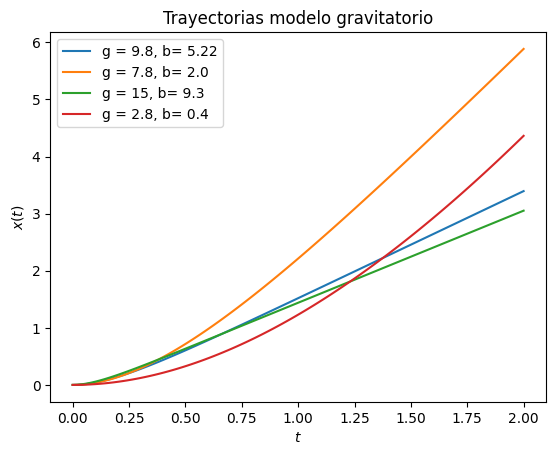
\includegraphics[width = 10 cm]{img/Trayectoria.png}
    \caption{Varias trayectorias con la dinámica gravitación sujeta a fricción para varias valores de los parámetros g,b.}
    \label{fig:trayectoria_gravedad}
\end{figure}

\subsection{Modelo Logístico}

Un modelo de crecimiento poblacional simple caracterizado por una ecuación diferencial es aquel que la tasa de cambio de la población es proporcional al tamaño actual de la población. Sea $P(t)$ el tamaño de la población al tiempo $t$. El modelo descrito es 
\begin{align}
    \frac{dP}{dt} = \lambda P(t),
    \label{3.1.2.01}
\end{align}
donde $\lambda$ es la tasa de crecimiento donde además se tiene la condición $P(0) = P_0$. 

La solución explicita al modelo en (\ref{3.1.2.01}) es
\begin{align*}
    P(t) = P_0 e^{\lambda t },
    % \label{3.1.2.02}
\end{align*}
que es una función creciente en el tiempo. Sin embargo, este modelo solo es valioso para intervalos de tiempo pequeños, ya que la tasa de crecimiento de una poblacional real tiende a decaer a medida que se consumen los recursos para su sustento.

Para saldar con la dificultad planteada, podemos modelar la tasa de crecimiento de una población considerando tanto al tamaño de la población como a los recursos aún presentes. Consideremos a $K$ como la capacidad de sustento, que se puede interpretar como la cantidad máxima de población que los actuales recursos permiten mantener, entonces esperamos que a medida que crece la población, la tasa de crecimiento de la misma decrezca.

El modelo que se propone es conocido como el modelo de crecimiento logístico. Este nos dice que el cambio de la población es proporcional al tamaño de la población misma así como a la proporción de recursos disponibles. Dicho modelo se puede escribir con la ecuación de Verhulst (\cite{zill2002ecuaciones}) 
\begin{align}
    \frac{dP}{dt} = rP\left(1- \frac{P}{K}  \right),
    \label{3.1.2.03}
\end{align}
donde $r$ es la tasa de crecimiento y $K$ la capacidad de sustento.

A pesar de que la ecuación diferencial del modelo de crecimiento logístico es no lineal tiene solución explicita. Notemos que la EDO pertenece a la familia de las EDO de Bernoulli (\cite{apostol1991calculus}), esto es tiene la forma
\begin{align*}
    \frac{dy}{dt} + P(x) y =Q(x) y^n,
\end{align*}
y además puede transformar a una EDO lineal de primer orden con el cambio de variable $u(x) = y ^{1-n}$.

Por tanto, del cambio $u(t) = P^{-1}$ obtenemos la solución explicita a (\ref{3.1.2.03})
\begin{align}
    P(t) = \frac{KP_0 e^{rt}}{K + P_0 \left(e^{rt}-1\right)},    
    \label{3.1.2.05}
\end{align}
donde verificamos que $\lim_{t \rightarrow \infty} = K $. 

Existe otra reparametrización del modelo lógistico que simplifica los cálculos en la metodología del problema inverso. Escribiremos que $X(t)$ sigue el crecimiento logístico si satisface
\begin{align}
    \frac{dX(t)}{dt} = \theta_1 X(t)\left(\theta_2 - X(t)\right).
    \label{3.1.2.06}
\end{align}
Con la parametrización dada por
\begin{align*}
    \theta_1 = \frac{r}{K}, \:\:\:\:\:\: \theta_2 = K,
\end{align*}
recuperamos la expresión dada en (\ref{3.1.2.03}).


\begin{figure}
    \centering
    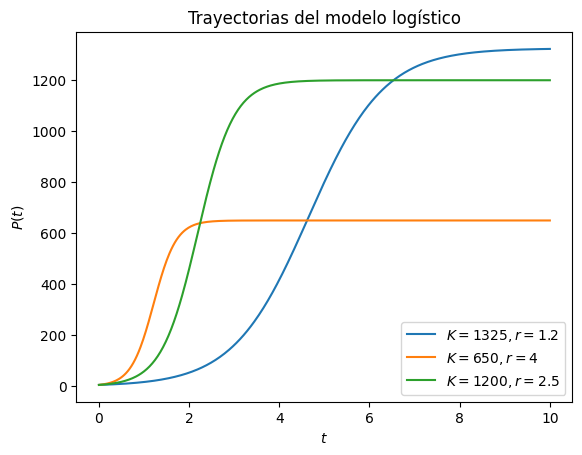
\includegraphics[width = 10 cm]{img/trayectoria_log.png}
    \caption{Varias trayectorias con la dinámica de crecimiento logístico para varias valores de los parámetros K,r.}
    \label{fig:trayectoria_logistico}
\end{figure}

En la Fig \ref{fig:trayectoria_logistico} se muestran varias trayectorias del crecimiento poblacional con diferentes parámetros usando la parametrización interpretable en términos de tasa de crecimiento $r$ y poblacional máxima $K$. Además, vemos que cada trayectoria es no decreciente y tiende asintóticamente al parámetro $K$. 



\subsection{Modelo SIR}

Los modelos epidemiólogos clasifican a la población en clases que distinguen si han tenido o no cierta enfermedad. Un modelo que captura con buena aproximación a varias enfermedades se es el modelo SIR. Este propone dividir a las $N$ personas de una población en tres grupos:
\begin{enumerate}
    \item Susceptible ($S$): Cantidad de personas que no han tenido la enfermedad ni están enfermas del brote de interés.
    \item Infectado ($I$): Son las personas que actualmente portan el patógeno y son además un vector de transmisión.
    \item Recuperado ($R$): Para aquellas personas que se han recuperado de la enfermedad y ya tienen inmunidad o también para aquellas que perecieron.
\end{enumerate}

Así, el modelo propuesto supone que la tasa de cambios de las personas susceptibles decrece proporcionalmente a la cantidad de infectados y la cantidad de susceptibles restantes. De igual forma, la cantidad de recuperados crece con una tasa proporcional a la cantidad de infectados. La dinámica del modelo SIR se da con el siguiente sistema de EDO's
\begin{align}
    \frac{dS}{dt} &= -\beta S I, \nonumber \\
    \frac{dI}{dt} &= \beta S I - \gamma I,
    \label{3.1.3.01} \\
    \frac{dR}{dt} &= \gamma I, \nonumber
\end{align}
donde $\beta$ es la tasa de infección, $\gamma$ es la tasa de recuperación y $S + I + R = N$ (\cite{weiss2013sir}).

La solución explicita para $S(t), I(t), R(t)$ no existe en general, por ello se requieren métodos numéricos (\cite{mathews2000metodos}) para resolver numéricamente para cada grupo y poder construir el forward map . La implementación de python usando la paquetería odeint se pude ver en \cite{jimenez2022metodos} y en \cite{griffiths2010numerical}. En la Fig. \ref{fig:trayectoria_SIR} tenemos un ejemplo para un solo caso del modelo SIR con tasa de infección $\beta = 0.009$ y tasa de recuperación $\gamma = 0.5$


\begin{figure}
    \centering
    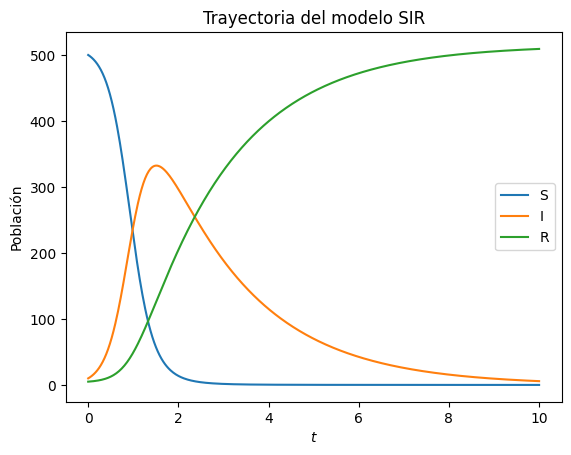
\includegraphics[width = 10 cm]{img/trayectoria_SIR.png}
    \caption{Trayectoria de cada grupo del modelo SIR con $\beta = 0.009$ y $\gamma = 0.5$.}
    \label{fig:trayectoria_SIR}
\end{figure}




% \section{Inferencia sin aproximación}
\section{Enfoque bayesiano al problema inverso}

Una vez establecidos los modelos sobre los que trabajaremos, nos enfocamos en abordar el problema inverso para los mismos. Para ello, es necesario tener a disposición una muestra de la trayectoria del modelo al cual deseamos inferir sus parámetros.

Según sea el caso, podemos realizar mediciones de caída de un objeto para ciertos tiempos, contar la cantidad de población para cada intervalo de tiempo, o observar los grupos de personas en un brote de cierto patógeno. Denotemos estas observaciones por $y_1, y_2, \cdots, y_n$. 

Sin embargo, no es fácil tener acceso a dicha muestra, por lo que optaremos por simular los datos directamente del modelo seleccionando los parámetros convenientemente y además agregar un ruido gaussiano. Es decir, tomamos $\theta \in \Theta$ fijo, luego consideramos los tiempos a los cuales corresponderá la muestra, denotados por $t_1, t_2, \cdots, t_n$. Posteriormente, con el forward map ordinario $F_{\theta}$ (sin aproximación por vecinos cercanos) generado según el modelo (ya sea analítico o numérico) evaluamos para cada tiempo (denotado por $F_{\theta}(t_i)$) y agregamos un ruido $\varepsilon_i \sim N(0,\sigma^2)$. Así la muestra considerada se constituye por
\begin{align}
    y_i = F_{\theta}(t_i) + \varepsilon_i,%\:\:\:\: \text{para } i = 1,2,\cdots,n.
    \label{3.2.01}
\end{align}
para $i = 1,2, \cdots, n$. Dicho de otra forma la muestra contemplada es
\begin{align}
    \left \{ (y_1,t_1), (y_2, t_2), \cdots, (y_n, t_n)\right \},
\end{align}
un conjunto de $n$ tuplas.


Una vez establecida la muestra $y_i$, ahora el propósito es abordar el problema inverso, esto es, buscamos $\theta$ tal que $y_i \approx F_{\theta}(t_i)$. Ya hemos estudiado el enfoque bayesiano al problema inverso en el capítulo 2, desde luego la implementación obtenida aquí sera inicialmente el caso de forward map ordinario.

\subsection{Distribución posterior}

En la teoría de la estadística bayesiana, el paradigma central se basa en obtener la distribución posterior de los parámetros de interés dada ciertas observaciones a las que hemos denotamos por $\mathbf{y} = (y_1,y_2,\cdots, y_n)$. 
En coordenadas canónicas, el vector de parámetros es $\theta = (\theta_1,\theta_2, \cdots, \theta_d) \in \mathbb{R}^d$. Recordemos de (\ref{2.2.04}) que la distribución posterior satisface la ecuación  
\begin{align}
    \pi(\theta|\mathbf{y}) \propto f(\mathbf{y}|\theta) \pi(\theta),
    \label{3.2.1.01}
\end{align} 
definida salvo una constante en términos de la verosimilitud y la distribución a priori. 

El análisis del calculo de la verosimilitud se trató en la sección 2 del capítulo 2. De la ecuación (\ref{2.2.03}) junto con (\ref{3.2.1.01})
\begin{align}
    \pi(\theta|\mathbf{y}) \propto \left(\frac{1}{2\pi \sigma^2}\right) ^{n/2}\exp \left \{  -\frac{1}{2\sigma^2}\sum_{i = 1}^{n} \left(y_i - F_{\theta}(t_i)\right)^2 \right \} \pi(\theta),
    \label{3.2.1.02}
\end{align}
rescatamos la distribución posterior en función del forward map, salvo una constante. De esta forma, resta discutir las cualidades deseadas para los modelos anteriormente descritos.

% Para obtener la verosimilitud, observemos de la ecuación (\ref{3.2.01}) que 
% \begin{align*}
%     \mathbf{y}_i \sim N(F_{\theta}(t_i)), \sigma^2)
% \end{align*}
% por lo que la verosimilitud para $\theta$ es la correspondiente al modelo normal, es decir
% \begin{align}
%     \mathcal{L} (\theta,\sigma) = f(\mathbf{y}|\theta) = \prod_{i = 1}^{n} \frac{1}{2\pi \sigma^2} \exp \left \{ -\frac{1}{2\sigma^2}\left(y_i - F_{\theta}(t_i)\right)^2 \right \} ,
% \end{align}
% simplificando
% \begin{align}
%     \mathcal{L}(\theta,\sigma) = \left(\frac{1}{2\pi \sigma^2}\right) ^{n/2}\exp \left \{  -\frac{1}{2\sigma^2}\sum_{i = 1}^{n} \left(y_i - F_{\theta}(t_i)\right)^2 \right \},
%     \label{3.2.1.02}
% \end{align}
% que es la verosimilitud en función de los parámetros $\theta$ y la desviación estándar $\sigma$. 

Para nuestro caso particular, todos los modelos propuestos en la sección precedente dependen de parámetros no negativos, es decir, $\theta_i \geq 0$ para toda $i = 1,\cdots, d$. Incluso algunos de ellos se tiene bastante certeza de su valor, que podría pensarse en ajustar una distribución a priori normal. Sin embargo, ajustar una normal conlleva a tener problemas en el soporte, por lo que puede pensarse en considerar una normal truncada a los positivos, sin embargo está complica innesariamente las expresiones para la distribución posterior. 

Finalmente, se opta por proponer distribuciones a priori gamma, debido a que existe una parametrización en la cual se asemeja a una distribución normal pero con el soporte adecuado. La distribución gamma que tiene por  máximo a $\theta_{i}^{*}$ y asemeja una normal es 
\begin{align}
    \theta_i \sim Gamma\left(\alpha_i, \frac{\theta_i^{*}}{\alpha_i} \right),
    \label{3.2.1.03}
\end{align}
con $\theta_i^{*}$ y $\alpha_i$ parámetros conocidos.

La parametrización de la $Gamma(\alpha,\beta)$ es tal que su función de densidad sea
\begin{align*}
    f(\theta|\alpha,\beta) = \frac{\beta^\alpha}{\Gamma(\alpha)} \theta^{\alpha-1} \exp \left \{ -\beta \theta\right \},
\end{align*}
con $\alpha,\beta$ conocidos.

Como $\theta_i$ se proponen independientes, entonces la distribución a priori para $\theta$ es
\begin{align}
    \pi(\theta|\alpha) &= \pi(\theta_1|\alpha_1) \cdots \pi(\theta_d|\alpha_d) \nonumber \\
    &= \prod_{i = 1}^{n} \left[\frac{1}{\Gamma(\alpha_i)}\left(\frac{\theta_i^{*}}{\alpha_i}\right) ^{\alpha_i} \theta_i^{\alpha_i -1} \exp \left \{ -\frac{\theta_i^{*}}{\alpha_i}\theta_i\right \}\right],
    \label{3.2.1.04}
\end{align}
desarrollando
\begin{align}
    &\pi(\theta|\alpha) =  \nonumber \\
    &\frac{1}{\Gamma(\alpha_1)}\left(\frac{\theta_1^{*}}{\alpha_1}\right) ^{\alpha_1} \theta_1^{\alpha_1 -1} \exp \left \{ -\frac{\theta_1^{*}}{\alpha_1}\theta_1\right \}  \cdots \frac{1}{\Gamma(\alpha_d)}\left(\frac{\theta_d^{*}}{\alpha_d}\right) ^{\alpha_d} \theta_d^{\alpha_d -1} \exp \left \{ -\frac{\theta_d^{*}}{\alpha_d}\theta_d\right \},
    \label{3.2.1.05}
\end{align}
con $\alpha = (\alpha_1,\cdots, \alpha_p)$ y $\theta^{*} = (\theta_1^{*}, \cdots , \theta_d^{*})$ conocidos.

Sustituyendo (\ref{3.2.1.04}) en (\ref{3.2.1.02}) se tiene la forma funcional de la distribución posterior
\begin{align}
    &\pi(\theta, \sigma|\mathbf{y}) \propto  \nonumber\\ &\left(\frac{1}{2\pi \sigma^2}\right) ^{n/2}\exp \left \{  -\frac{1}{2\sigma^2}\sum_{i = 1}^{n} \left(y_i - F_{\theta}(t_i)\right)^2 \right \} \prod_{i = 1}^{n} \left[\frac{1}{\Gamma(\alpha_i)}\left(\frac{\theta_i^{*}}{\alpha_i}\right) ^{\alpha_i} \theta_i^{\alpha_i -1} \exp \left \{ -\frac{\theta_i^{*}}{\alpha_i}\theta_i\right \}\right] 
    \label{3.2.1.06}
\end{align}

Notemos que la distribución en (\ref{3.2.1.06}) no pertenece a una familia conocida. Para lidiar con este problema usamos métodos Monte Carlo. Más precisamente, podemos simular de la distribución posterior (\ref{3.2.1.06}).


% \subsection{Forward map}
\subsection{Simulación con MCMC forward map ordinario}

Al incursionar a la estadística bayesiana se aprende que se puede obtener la distribución posterior por medio del famoso análisis conjugado. Es decir se propone una distribución a priori convenientemente para que la distribución posterior pertenezca a la misma familia. Sin embargo, el análisis conjugado puede ser no trivial o incluso no existir. Por ello es que simular de la distribución posterior con MCMC (Markov Chain Monte Carlo) es la via optima para tener una muestra $(X_i, i \in \{1,\cdots, T\})$ de dicha distribución, con la podemos estimar cualquier momento de la distribución. Si estamos interesados en obtener la media de $X$, en beneficio de la ley de grandes números (\cite{van2000asymptotic}), podemos estimar como
\begin{align}
    \mathbb{E}\left [X\right ] \approx \frac{1}{T}\sum_{i = 1}^{T} X_i
\end{align}
De igual forma si estamos interesados en la media del estadístico $h(X)$ para un función $h$ arbitraria, se estima por
\begin{align}
    \mathbb{E}\left [h(X)\right ] \approx \frac{1}{T} \sum_{i=1}^{T} h(X_i)
    \label{3.2.2.01}
\end{align}
donde $X_i$ es la $i$-ésima simulación de la distribución posterior por Metropolis-Hastings.

La distribución objetivo que se implementa en el MCMC es la distribución posterior (\ref{3.2.1.06}). Recordemos que la distribución posterior depende del forward map $F_{\theta}(t_i)$ obtenido de evaluar los tiempos de la muestra. Recordemos que $F_{\theta}(t_i)$ es la version discretizada de $F_{\theta}$. Sea $\theta \in \mathbb{R}^d$ la función
\begin{align}
    \theta  \mapsto F_{\theta} = x(t) 
\end{align}
tal que $x(t)$ es la solución de la ecuación diferencial ordinaria $x(t) = G(t,x(t),x'(t),x''(t)\cdots)$ del modelo bajo consideración.

\subsubsection{Simulación del modelo gravitatorio}

Para poder hacer simulaciones, es necesario determinar completamente la distribución posterior. El Forward map para el modelo gravitatorio es $F_{\theta} = F(g,b) = x(t)$ con la ecuación diferencial de la dinámica gravitacional dada en (\ref{3.1.03}) o equivalentemente en (\ref{3.1.12}). 

Además, es necesario saber como abordar el caso de la desviación estándar $\sigma$. En esencia existen dos formas, pensar en $\sigma$ como parámetro conocido, por lo que no es necesario hacer inferencia, manteniendo la distribución posterior tal como se ha detallado. En el otro caso es para $\sigma$ desconocida, al no tener certeza de su valor esta es agregada a los parámetros a inferir. Siguiendo el paradigma bayesiano, se establece una distribución a priori para $\sigma$ independiente de la distribución a priori para $\theta$. En otras palabras, ahora la distribución posterior depende de $d+1$ parámetros. Sin embargo para fines de esta tesis, nos abstendremos de los casos en los que $\sigma$ es desconocida.

De esta manera, la distribución posterior (\ref{3.2.1.06}) tendrá como variables unicamente al vector de parámetros $\theta$, al ser una EDO dependiente solamente de $g$ y $b$ se sigue que $\theta = (g,b)$ siendo un vector en $\mathbb{R}^{d}$ con $d = 2$. Además es necesario definir las constantes para las distribuciones a priori gamma.

Consideremos las distribuciones a priori (\ref{3.2.1.03}) como
\begin{align}
    g \sim Gamma \left(\alpha, \frac{\theta_1^{*}}{\alpha}\right) \\
    b \sim Gamma \left(\beta, \frac{\theta_2^{*}}{\beta}\right) 
\end{align}
con $\alpha = 10$, $\beta = 1.1$ con máximo en $\theta_1^{*} = 10$ y $\theta_2^{*} = 2$. Podemos observar las distribuciones a priori en la Fig. \ref{Fig. 3.2.2.01}.

\begin{figure}[H] 
    \centering 
    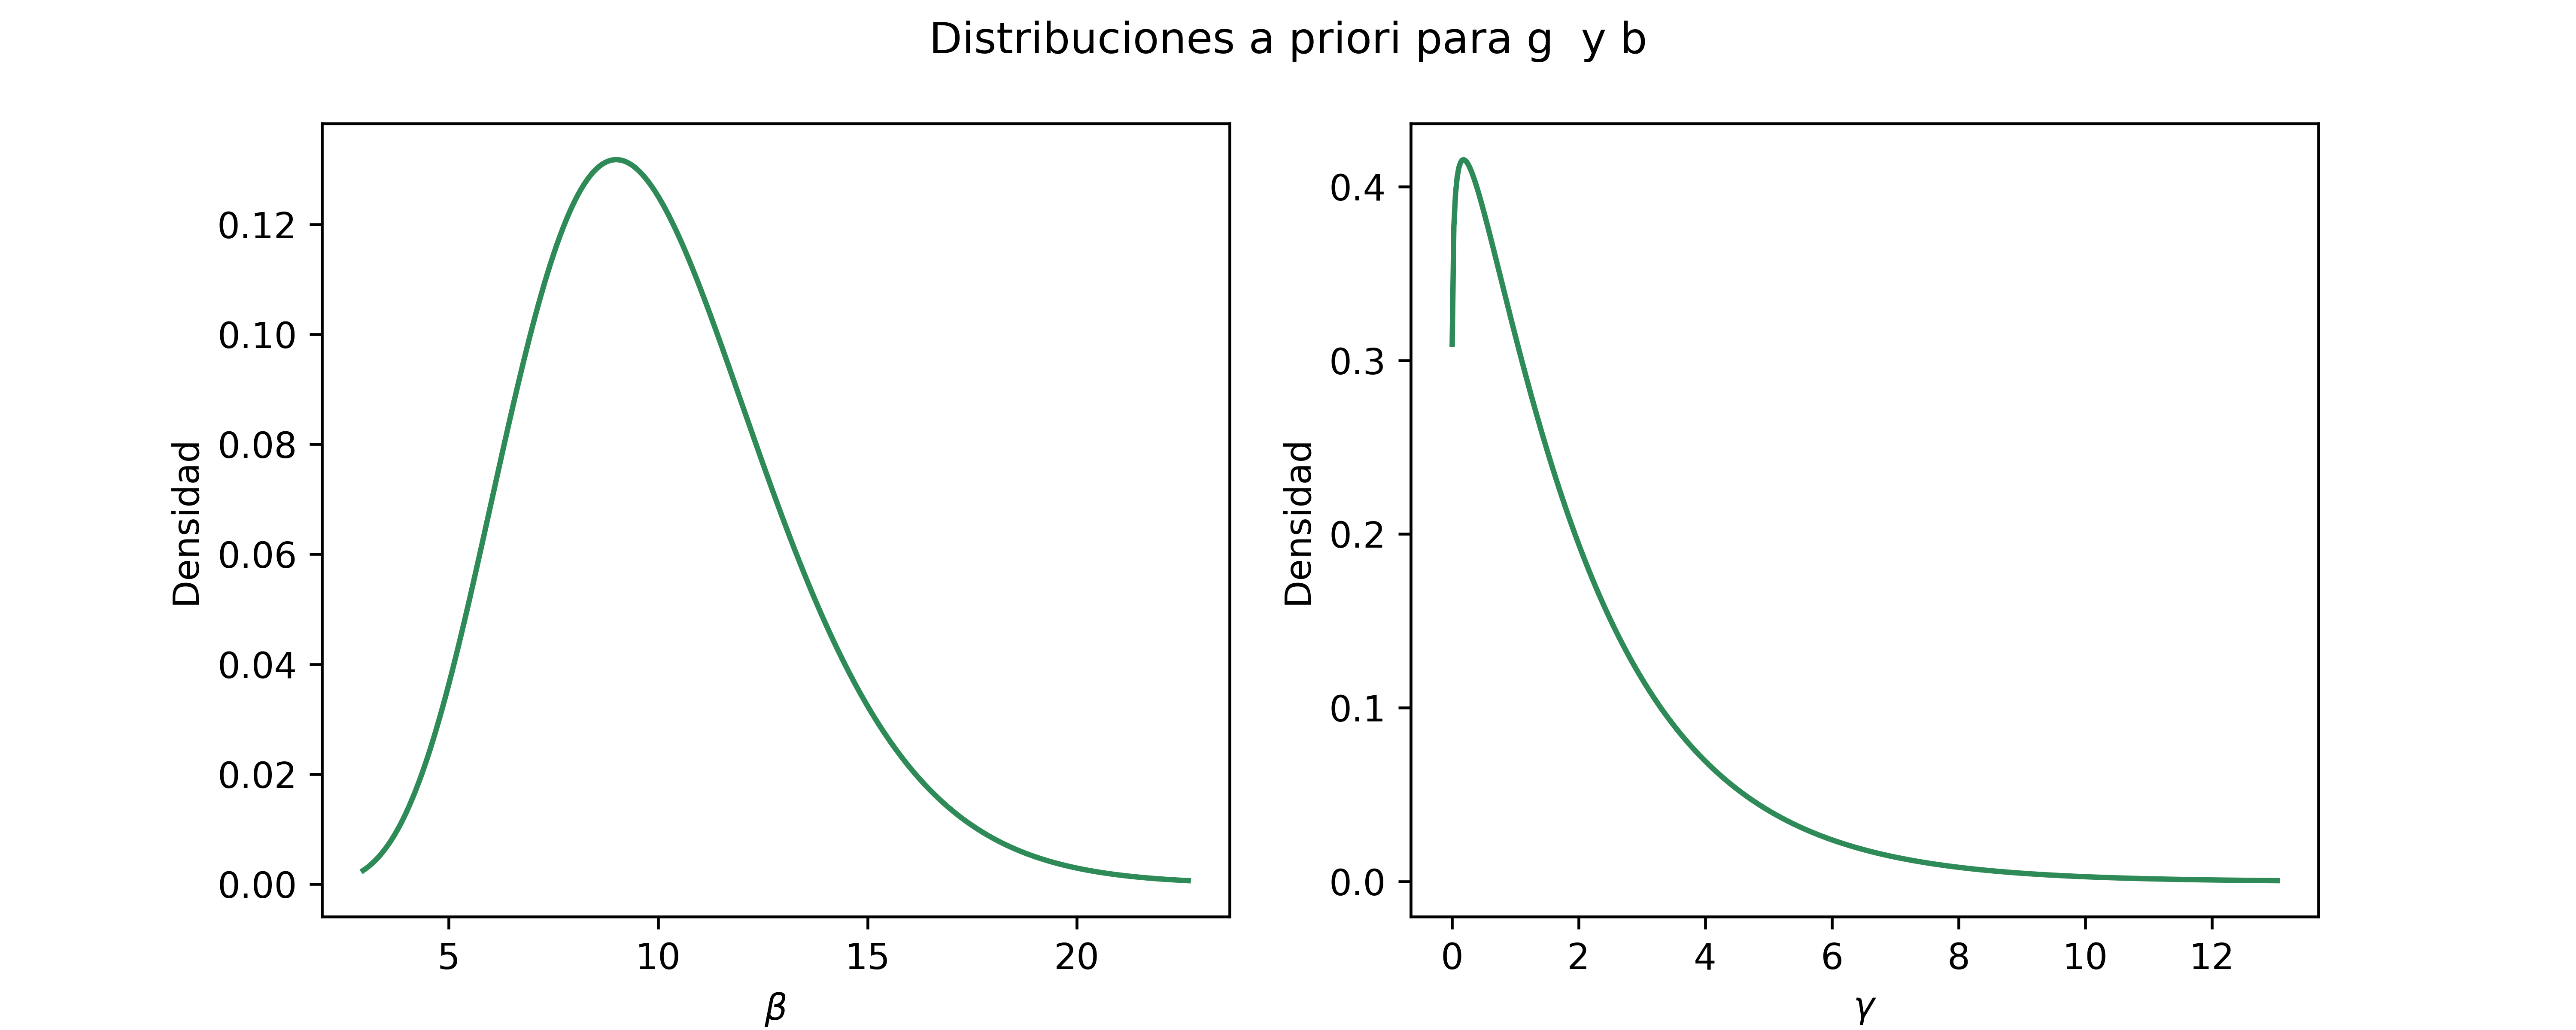
\includegraphics[width = 15 cm]{img/Exp_Central_gravedad_sigma/Figuras/Generales/Apriori_gravedad_sigma.png}
    \caption{Distribuciones marginal a priori para el parámetro $g$ (izquierda) y $b$ (derecha).}
    \label{Fig. 3.2.2.01}
\end{figure} 

Ahora, generamos una muestra $\mathbf{y}$ del forward map gravitatorio y agregamos un ruido gaussiano con $\sigma = 0.1$ obteniendo la muestra como en la Fig. \ref{Fig. 3.2.2.02}.

\begin{figure}
    \centering 
    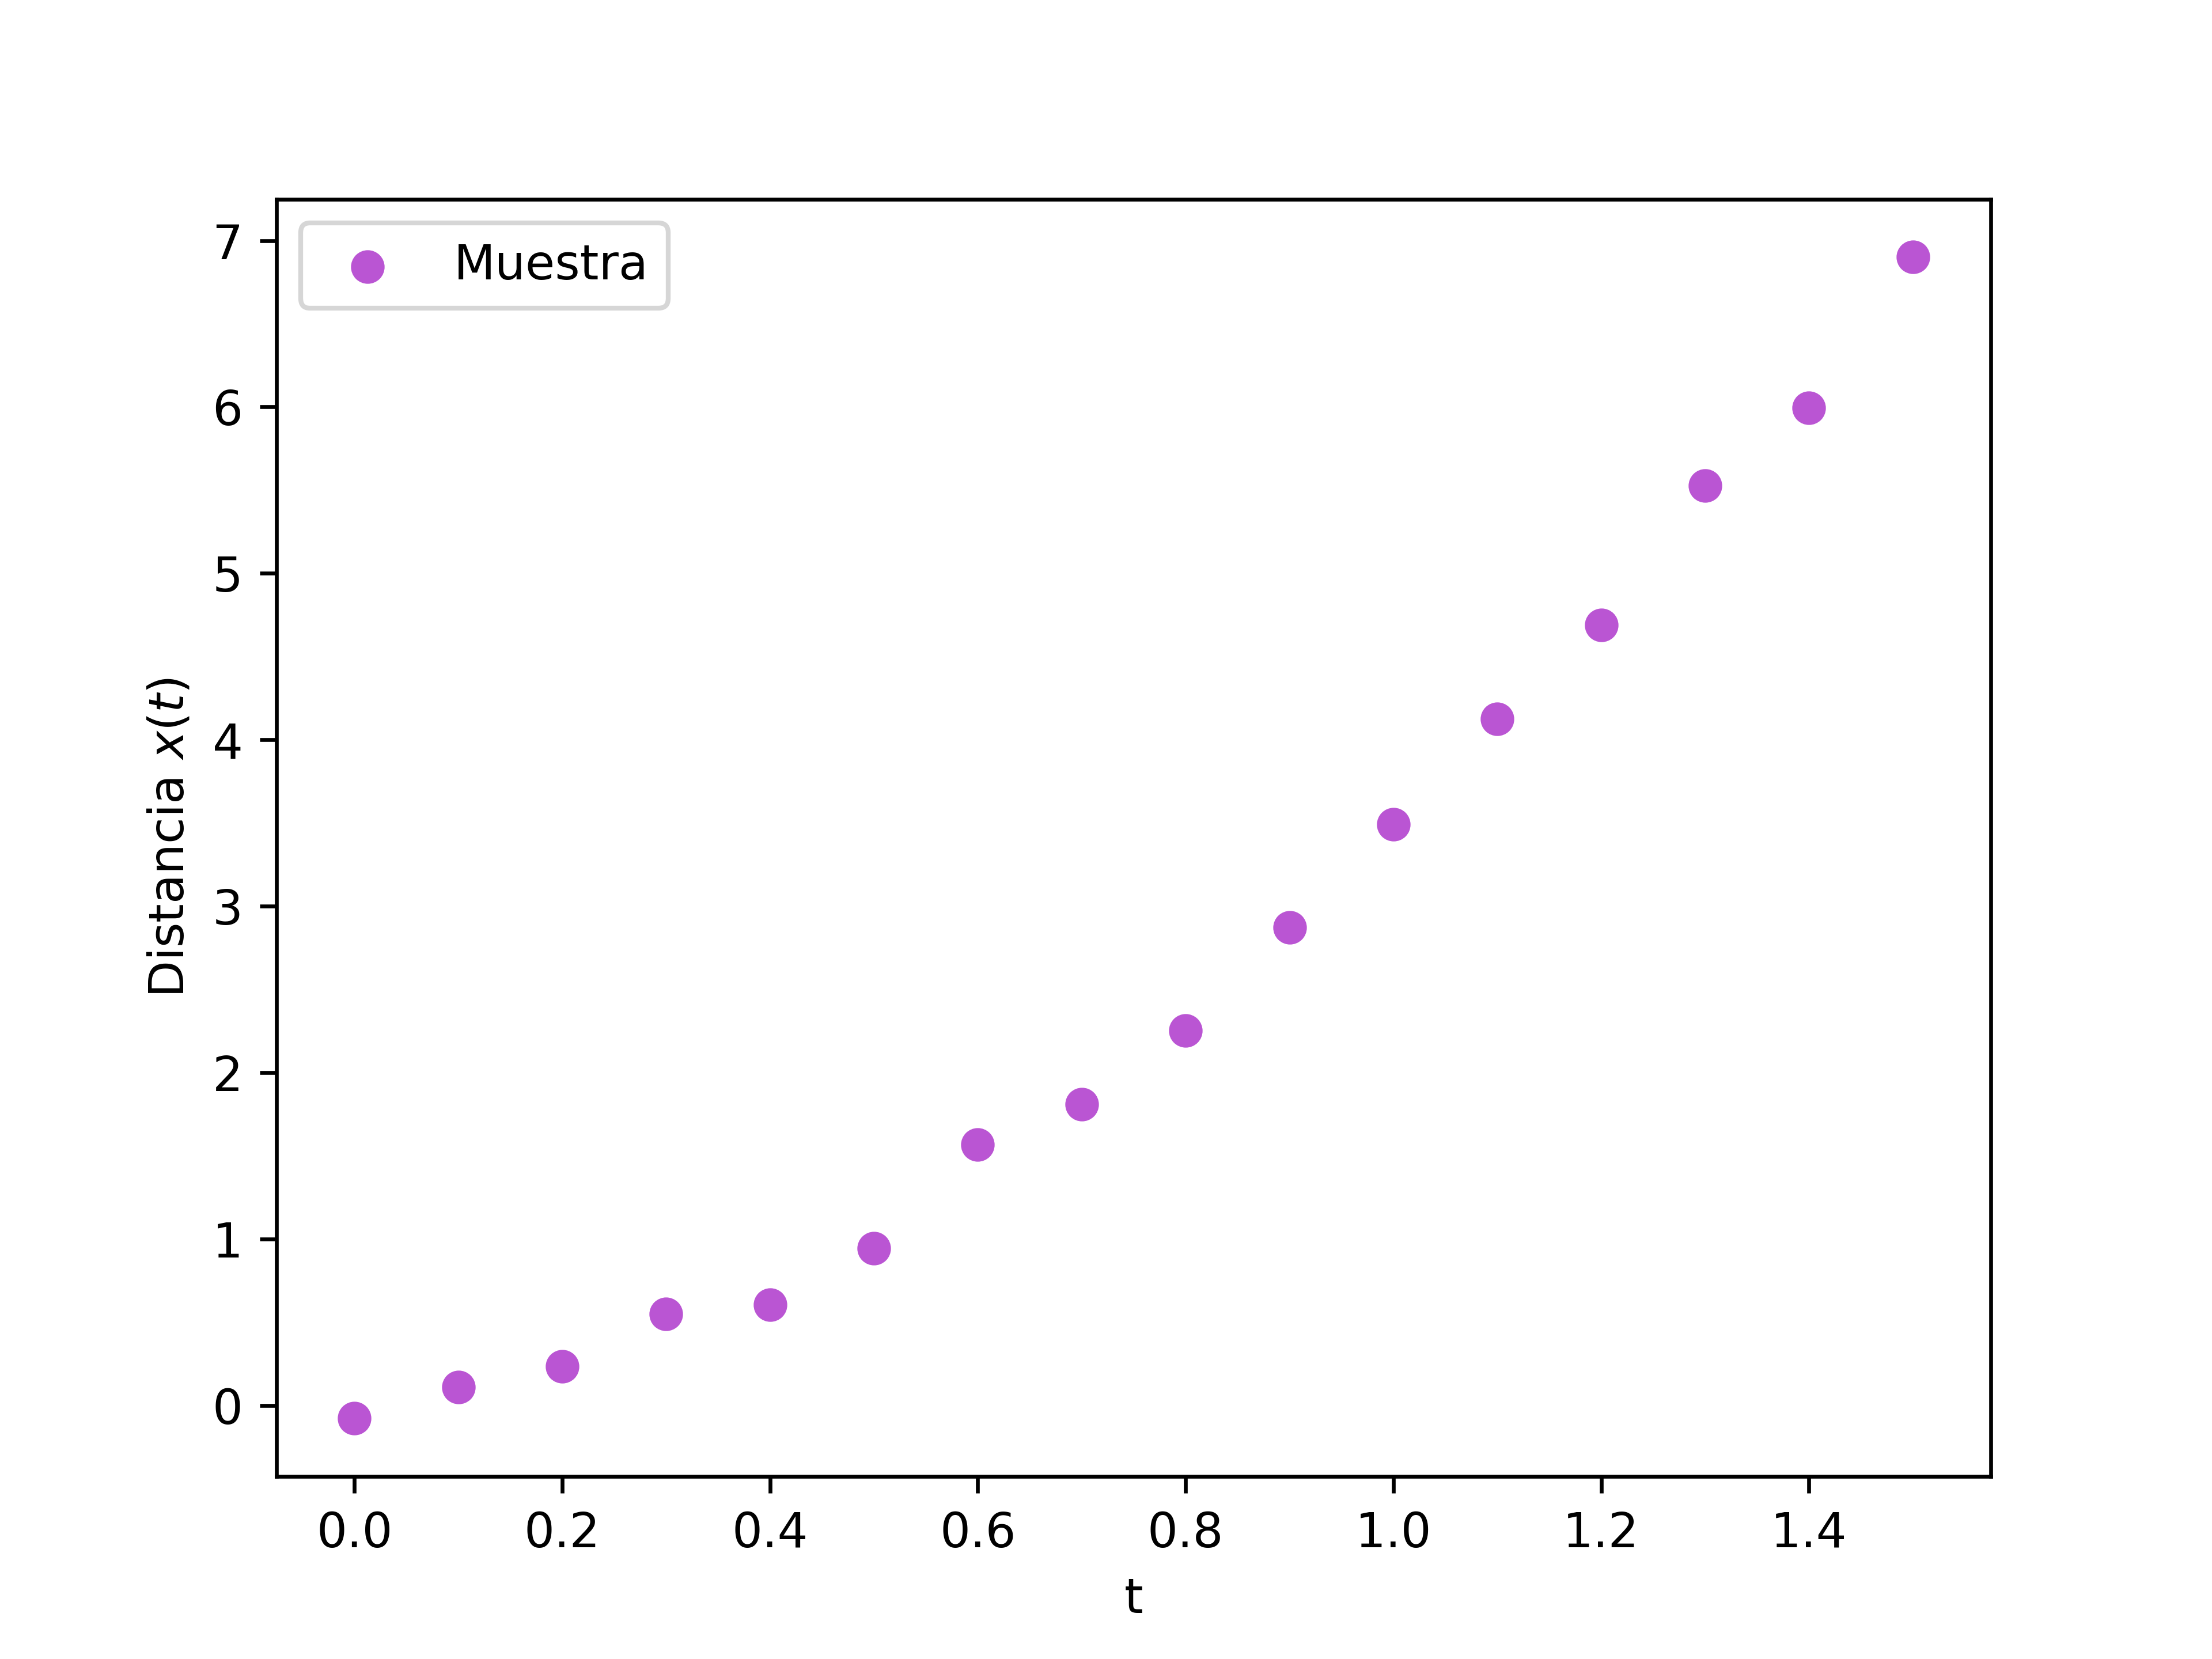
\includegraphics[width = 10 cm ]{img/Exp_Central_gravedad_sigma/Figuras/Generales/Muestra_gravedad_sigma.png} 
    \caption{Muestra $\mathbf{y}$ del modelo gravitatorio.}
    \label{Fig. 3.2.2.02}
\end{figure} 

Luego, con la metodología propuesta, usando el algoritmo MCMC Metropolis-Hastings (\cite{christen2010general}) para una cadena de tamaño $T = 600,000$ y un burn in de 20,000 tenemos que la trayectoria seguida en el espacio de parámetros $\theta = (g,b)$ para la distribución posterior (conjunta) es el mostrado en la Fig. \ref{Fig. 3.2.2.03}. Notemos que dicha posterior tiene alta correlación entre parámetros. Esto tiene la interpretación física que para valores altos de $g$ es necesario tener más fricción $b$ con el medio para la misma trayectoria $\mathbf{y}$.

\begin{figure}
    \centering 
    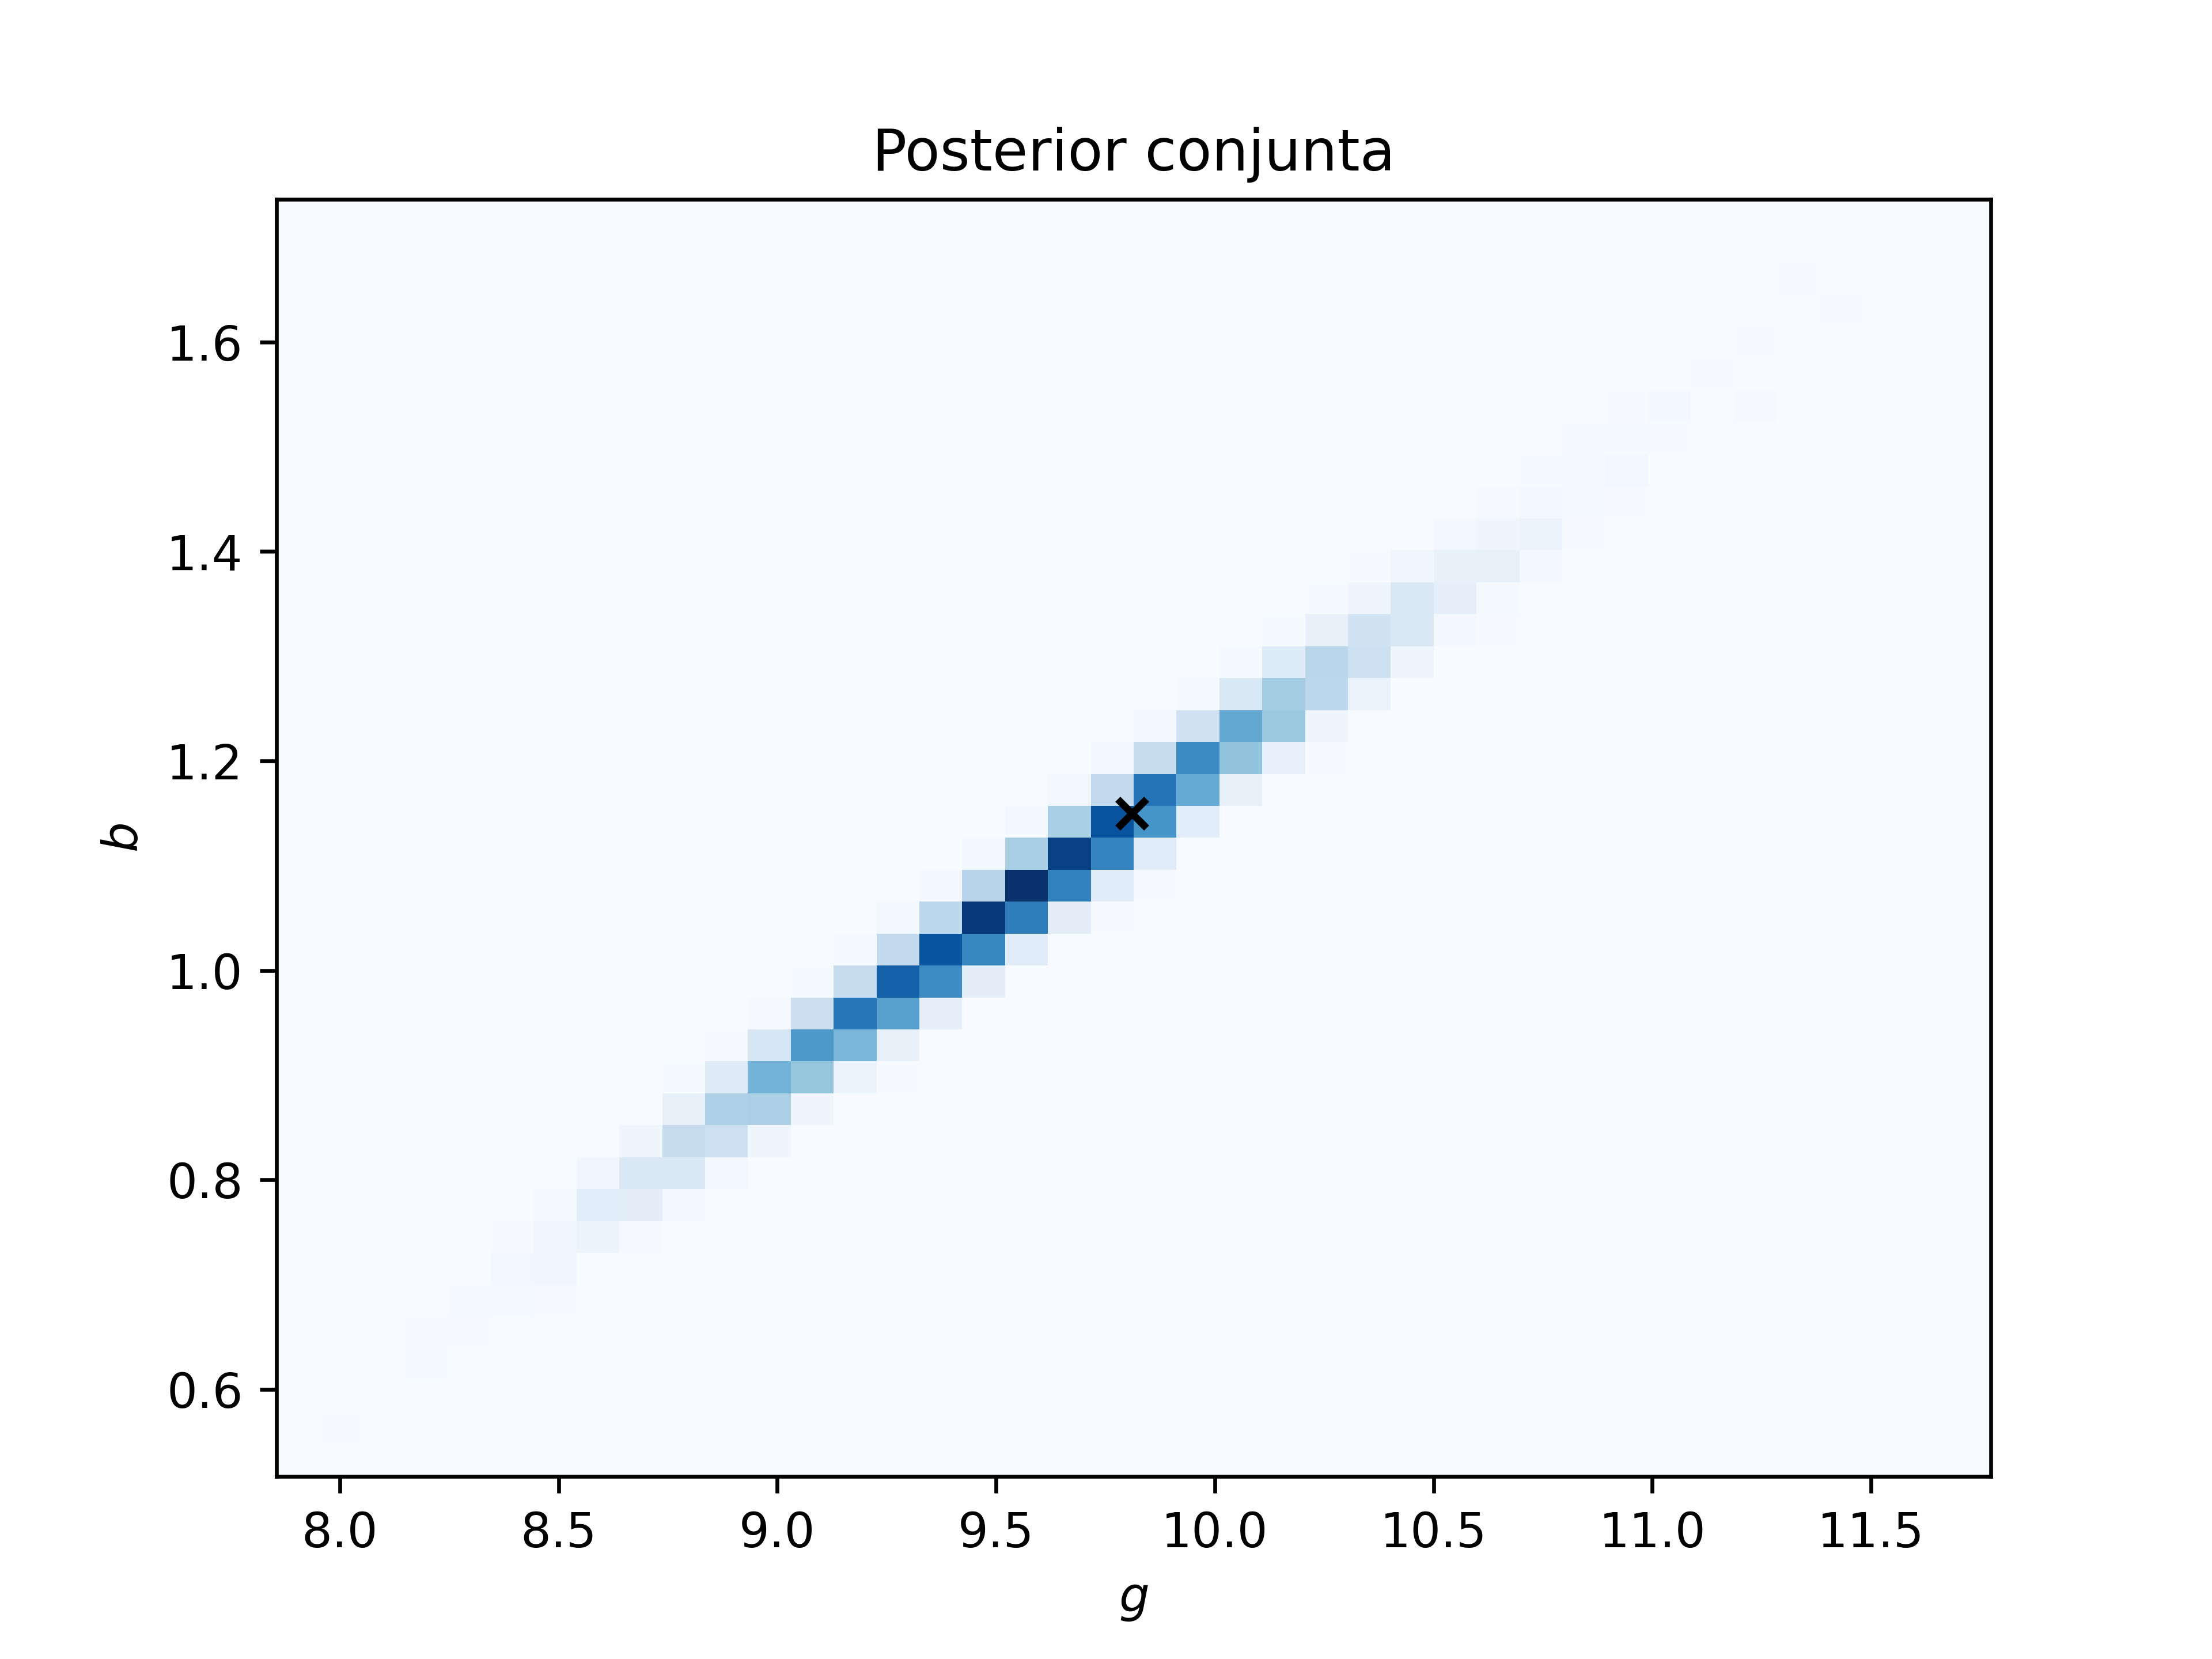
\includegraphics[width = 10 cm ]{img/Exp_Central_gravedad_sigma/Figuras/Generales/Conjunta_gravedad_sigma.png} 
    \caption{Estimación de la distribución posterior conjunta por método MCMC Metropolis-Hastings.}
    \label{Fig. 3.2.2.03}
\end{figure} 

Es de interés las marginales de la distribución posterior. Dado que la simulación de la cadena es bidimensional, de (\ref{3.2.2.01}) tomamos $h_1(X_1,X_2) = 1_{\{X_1\}}$ y $h_2(X_1,X_2)= 1_{\{X_2\}}$, dicho de otra forma, simplemente tomamos el histograma sobre una componente de la cadena dada por MCMC. Podemos ver las estimaciones a las distribuciones marginales posteriores para los parámetros $g$ y $b$ en  Fig. \ref{Fig. 3.2.2.04} y Fig. \ref{Fig. 3.2.2.05}

\begin{figure}[h]
    \centering
    \subfloat[Subfigure 1 list of figures text][Posterior para $g$.]{
    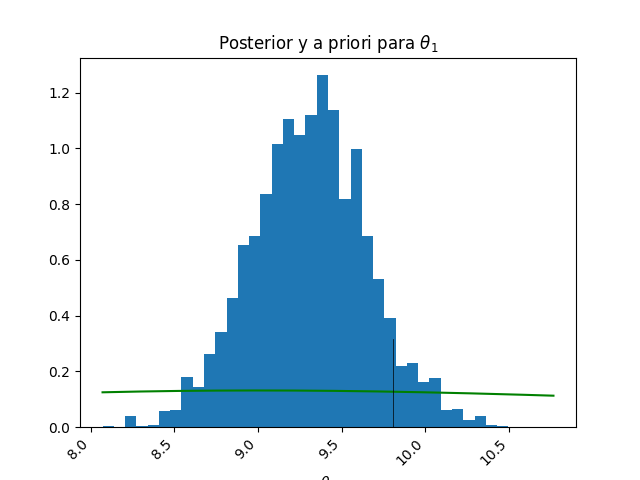
\includegraphics[width=0.4\textwidth]{img/Exp_Central_gravedad_sigma/Figuras/Generales/Post_theta1_gravedad_sigma.png}
    \label{Fig. 3.2.2.04}}
    \qquad
    \subfloat[Subfigure 2 list of figures text][Posterior para $b$.]{
    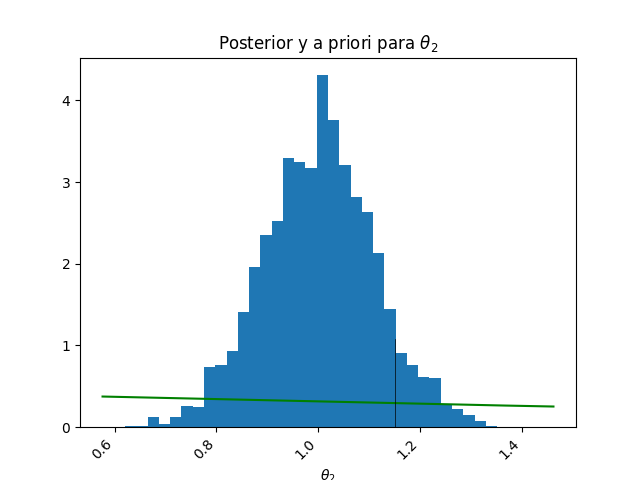
\includegraphics[width=0.4\textwidth]{img/Exp_Central_gravedad_sigma/Figuras/Generales/Post_theta2_gravedad_sigma.png}
    \label{Fig. 3.2.2.05}}
    \caption{Distribución posterior (azul) y distribución a priori (verde) para el parámetros $g$ y $b$ del modelo gravitatorio. }
    \label{Fig. 3.2.gravedad.theta}
\end{figure}


% \begin{figure}
%     \centering 
%     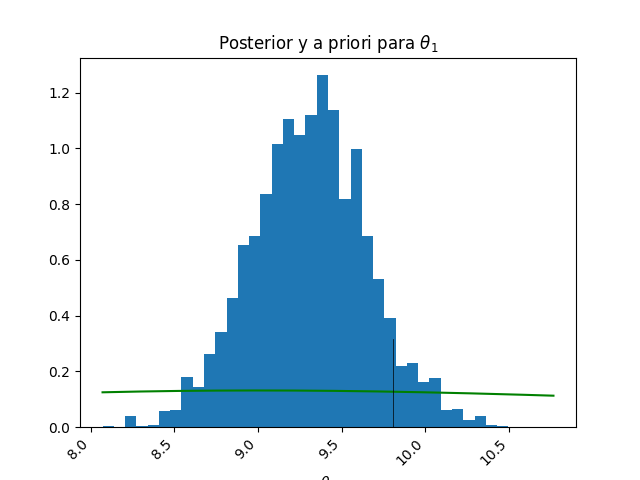
\includegraphics[width = 10 cm ]{img/Exp_Central_gravedad_sigma/Figuras/Generales/Post_theta1_gravedad_sigma.png} 
%     \caption{Distribución posterior (azul) y distribución a priori (verde)para el parámetros $g$.}
%     \label{Fig. 3.2.2.04}
% \end{figure} 

% \begin{figure}
%     \centering 
%     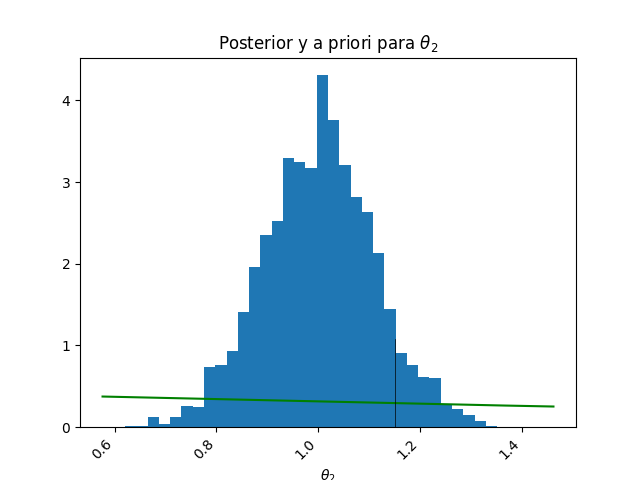
\includegraphics[width = 10 cm ]{img/Exp_Central_gravedad_sigma/Figuras/Generales/Post_theta2_gravedad_sigma.png} 
%     \caption{Distribución posterior (azul) y distribución a priori (verde) para el parámetro $b$. }
%     \label{Fig. 3.2.2.05}
% \end{figure} 

Finalmente, es de interés observar la distribución que puede generar las curvas predictivas. Es decir, de la cadena $X_t$ fruto de MCMC, tomamos submuestreos en intervalos $X_{[iN,(i+1)N]}$ para tomar estimaciones puntuales (media) de $g$ y $b$ y así aplicar el forward map para cada estimación. Dicho de otra forma, la información obtenida de la distribución posterior se desea transmitir directamente a la trayectoria, generando así distribuciones sobre las mismas.

\begin{figure}
    \centering 
    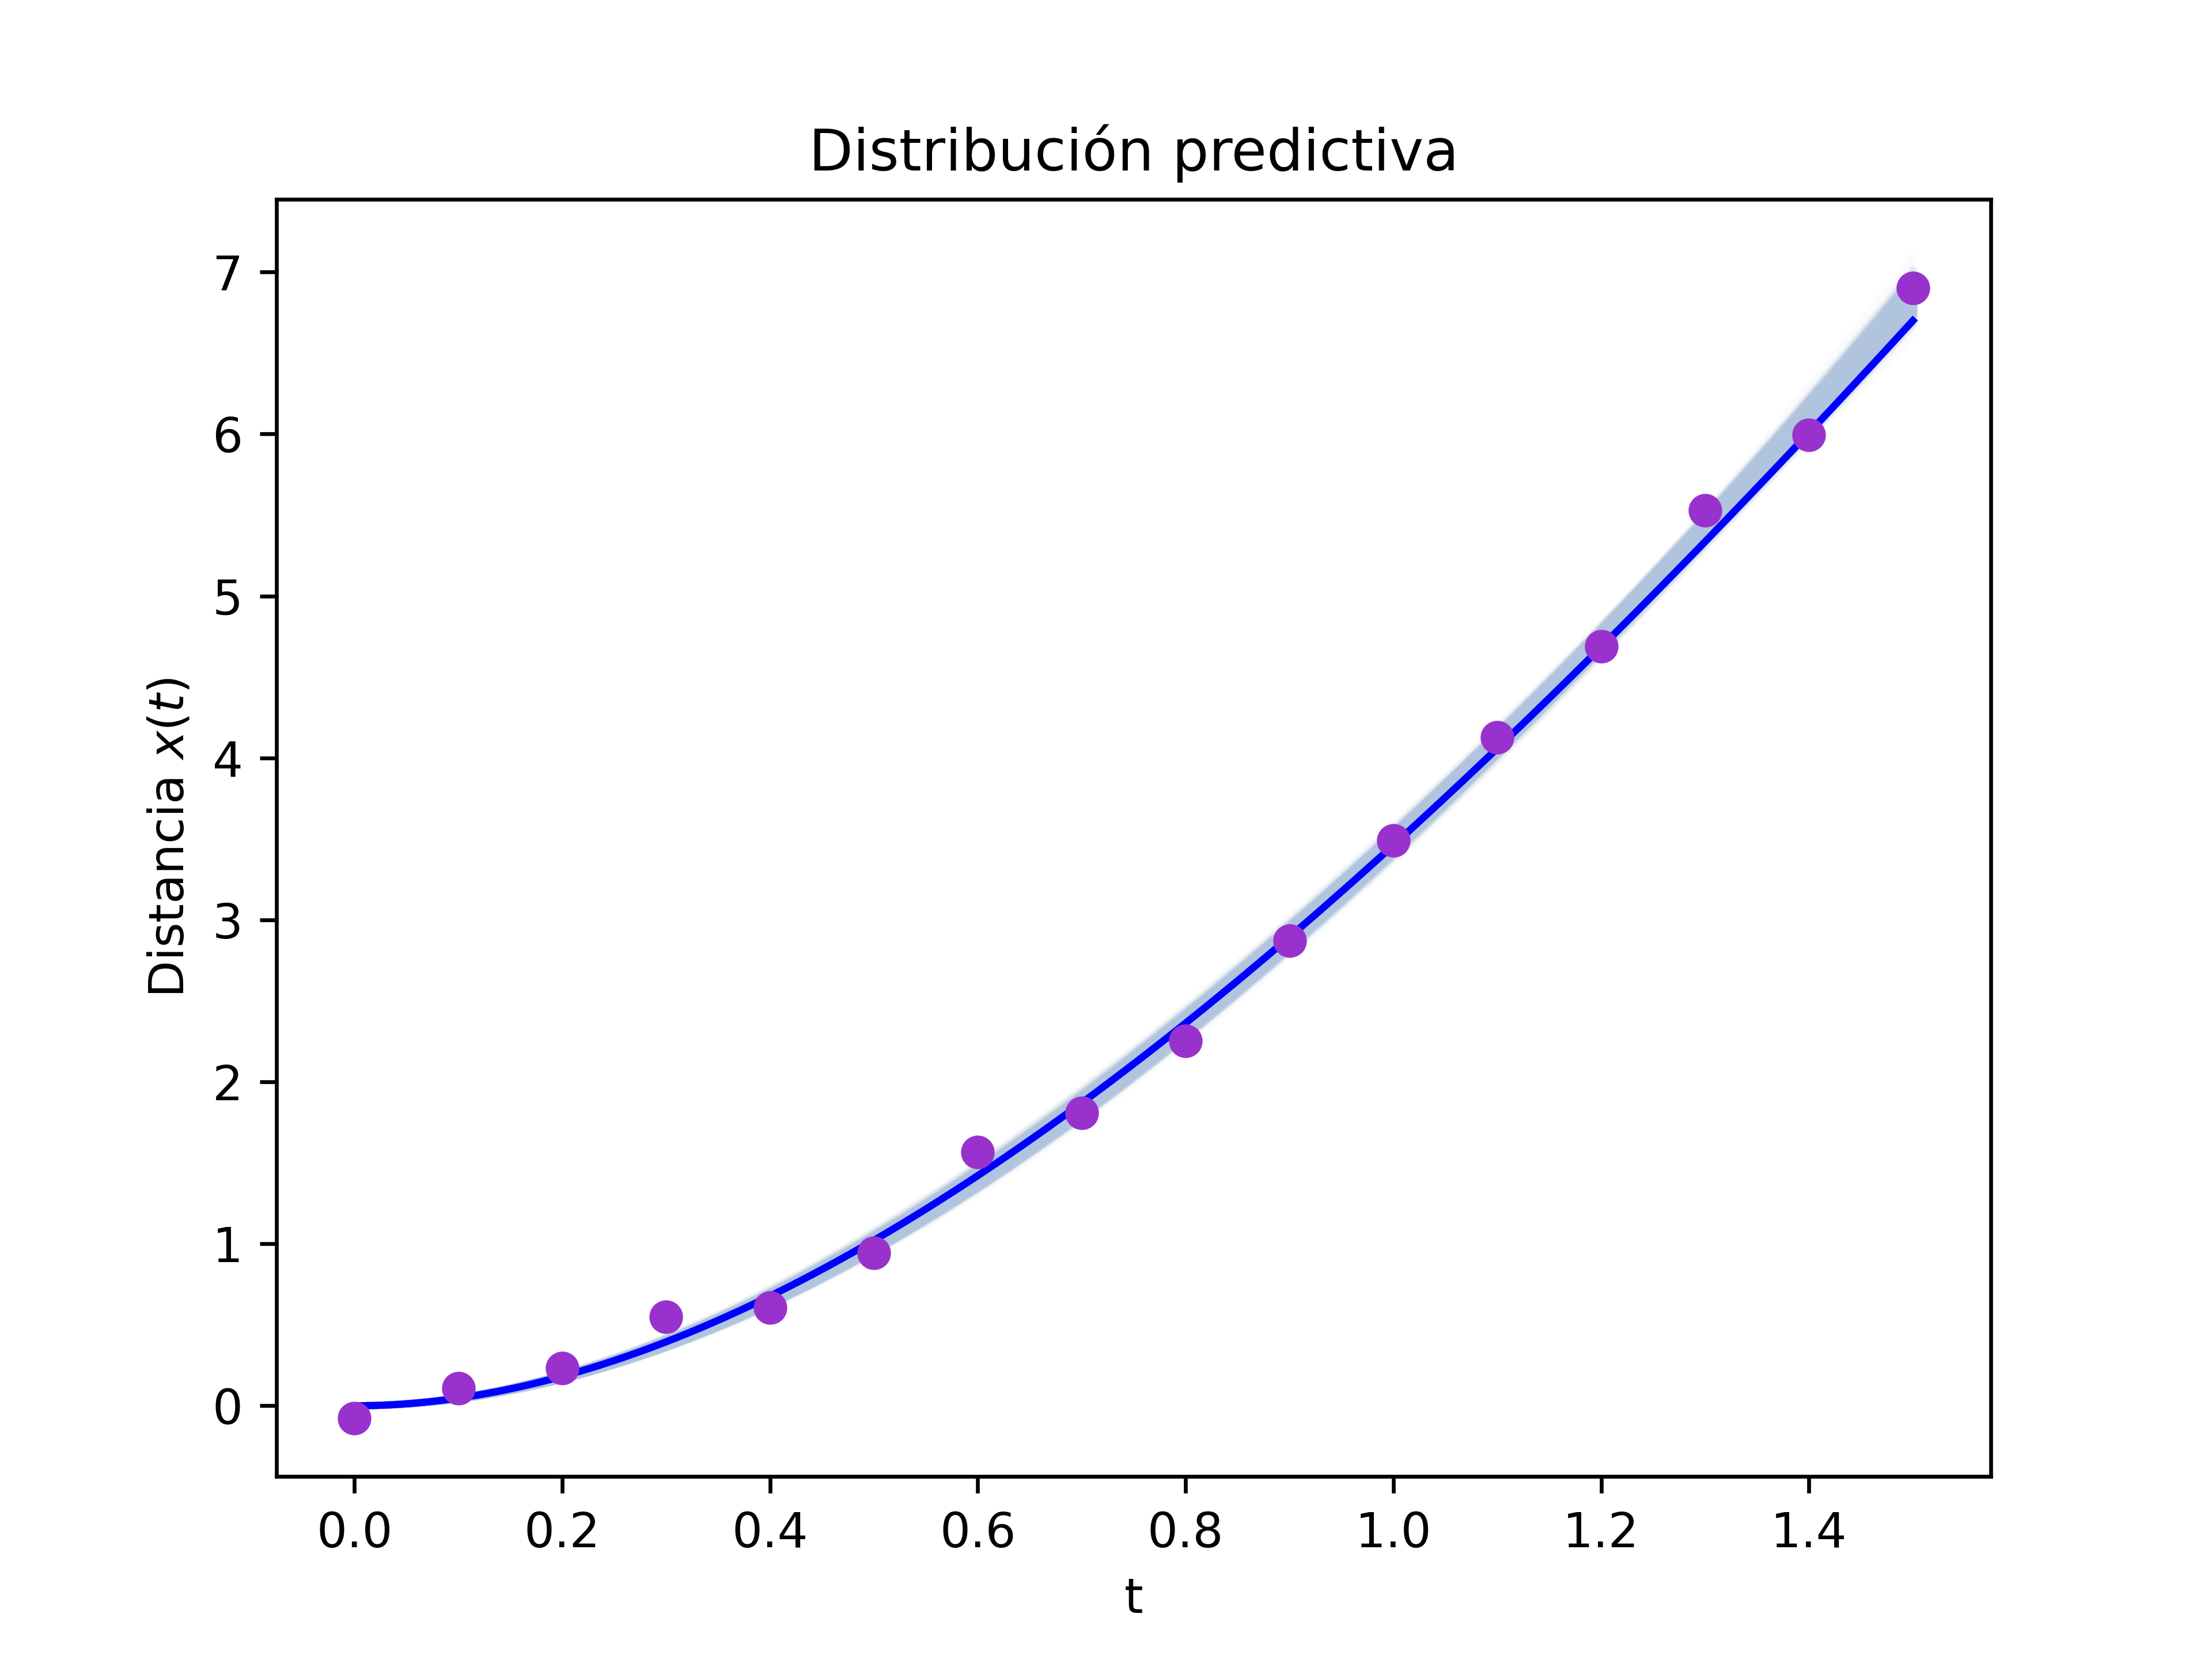
\includegraphics[width = 10 cm ]{img/Exp_Central_gravedad_sigma/Figuras/Generales/Predictiva_gravedad_sigma.png} 
    \caption{Distribución predictiva para el modelo gravitatorio}
    \label{Fig. 3.2.2.06}
\end{figure} 

En la Fig. \ref{Fig. 3.2.2.06} se muestra en azul claro los distintos forward map $F_{\theta}$ con varias realizaciones de $\theta|\mathbf{y}$ dada por la estimación de la distribución posterior por Metropolis-Hastings, mientras que en azul oscuro se muestra el forward map de partida, es decir, de donde se realizaron las simulaciones para generar $\mathbf{y}$ (morado). Por tanto, notamos que de cierta forma, la información de la distribución posterior contiene a la simulación inicial.

\begin{figure}[H]
    \centering 
    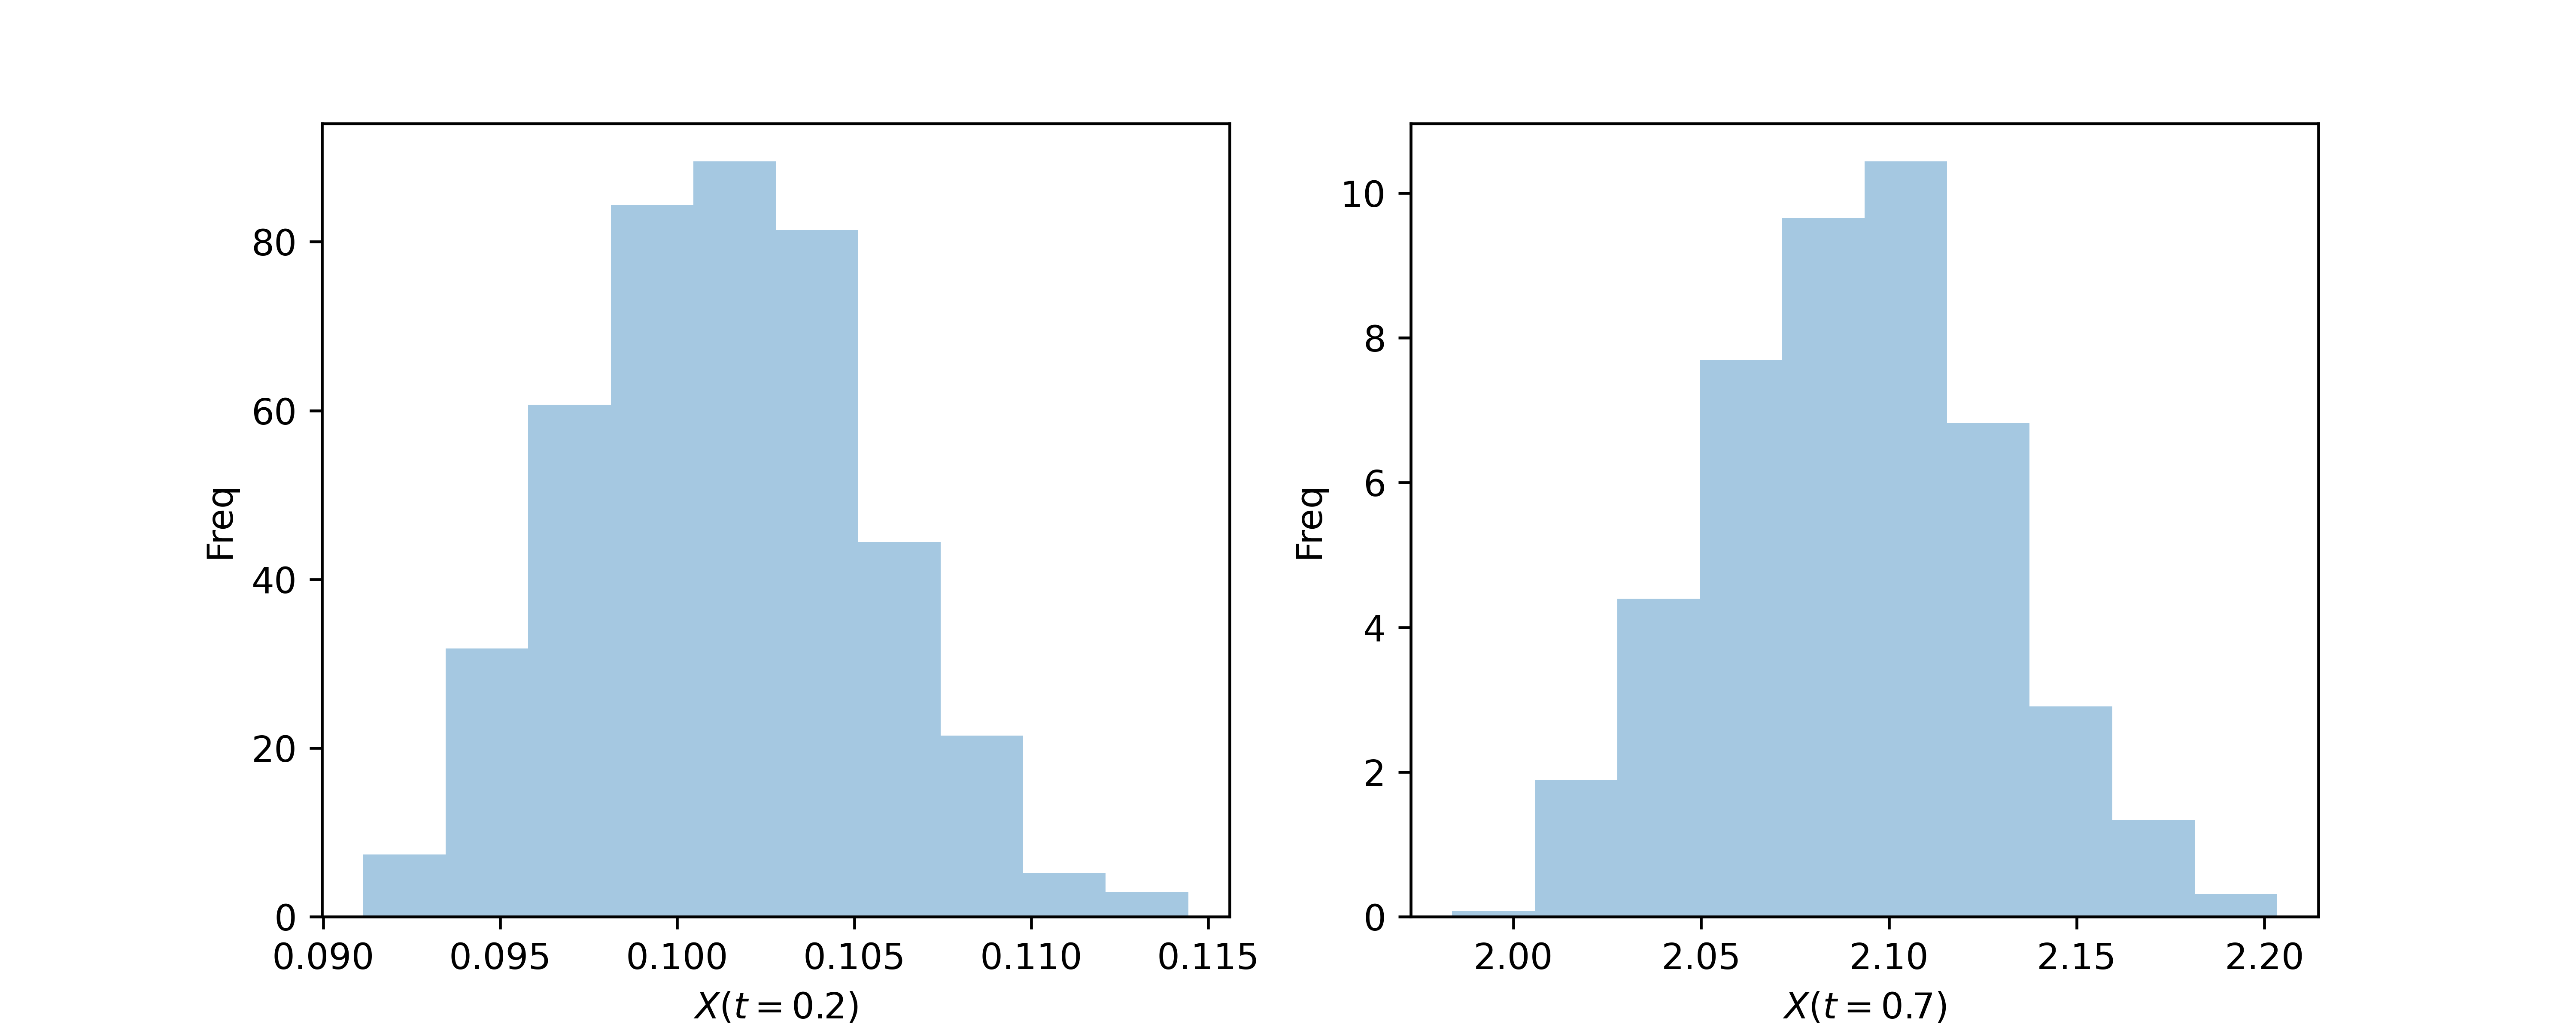
\includegraphics[width = 15 cm]{img/Exp_Central_gravedad_sigma/Figuras/Generales/TiempoFijo_gravedad_sigma.png} 
    \caption{Distribución predictiva del modelo gravitatorio para los valores de tiempo de 0.2s y 0.7s.}
    \label{Fig. 3.2.2.07}
\end{figure} 

Más aún, para ejemplificar la distribución predictiva, considere dos valores fijos de $t$ y tomese cortes verticales de la distribución predictiva. En la Fig. \ref{Fig. 3.2.2.07} nos muestra para el tiempo $t = 0.2 s$ y $t = 0.7s$ la distribución de probabilidad de la posición de la partícula afectada por la gravedad en ese momento de tiempo. 

\subsubsection{Simulación del modelo logístico}

En el modelo gravitacional tenemos un ejemplo de simulación del problema inverso donde las unidades de los parámetros difieren por un orden de magnitud a lo sumo, ya que las estimaciones del parámetro $g$ es aproximadamente 10 veces más grande que las estimaciones del parámetro $b$ en el sistema de unidades métrico decimal. Por tanto, es de interés trabajar un modelo cuyas estimaciones de los parámetros tengan un amplio margen de diferencia. El modelo logístico con la parametrización dada en (\ref{3.1.2.06}) el parámetro $\theta_2$ difiere en seis ordenes de magnitud respecto al parámetro $\theta_1$ \footnote{Para una población suficientemente grande y con una moderada tasa de crecimiento.}. En secciones posteriores retomaremos algunos comentarios respecto a esta clase de modelos.

Siguiendo la metodología ordinario para la resolución del problema inverso en el modelo, con la base de datos simuladas del mismo considerando $\theta_1 = 0.001$ y $\theta_2 = 1000$ con un ruido gaussiano aditivo de desviación estándar $\sigma = 30$ graficado en la Fig. \ref{Fig. 3.2.log.muestra}.

\begin{figure}[H] 
    \centering 
    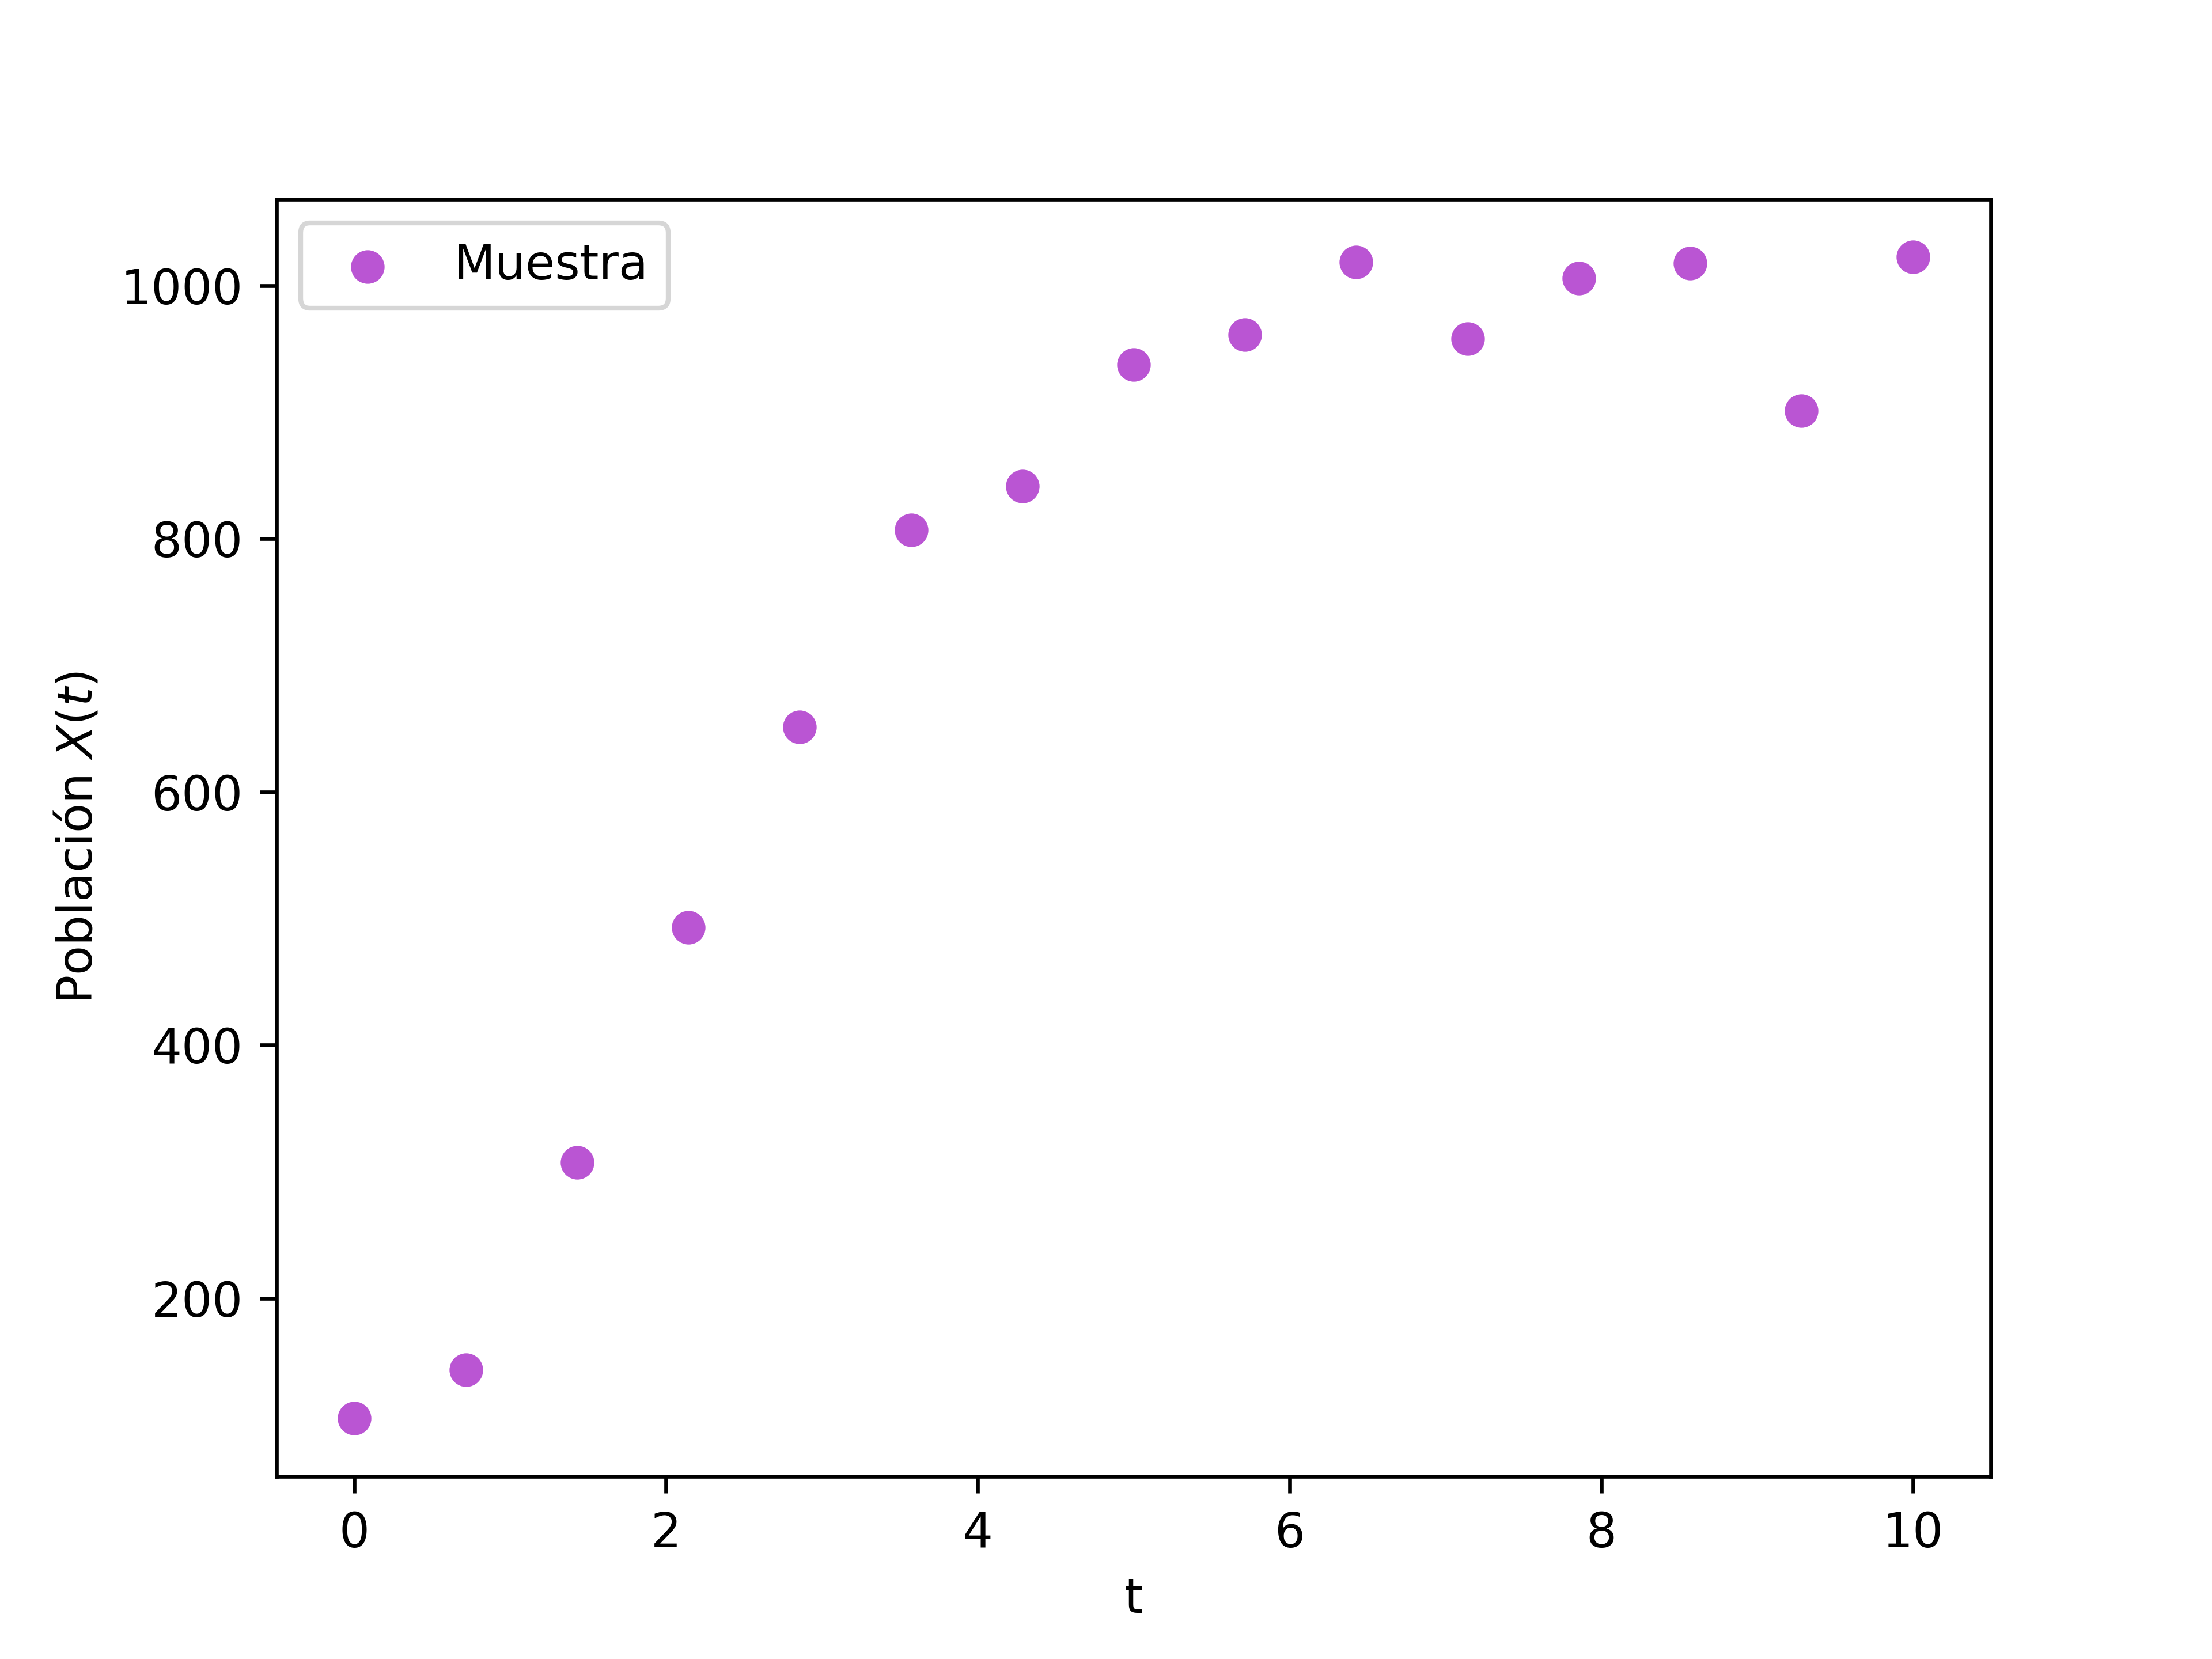
\includegraphics[width = 10 cm ]{img/Exp_Central_logistico_sigma/Figuras/Generales/Muestra_logistico_sigma.png} 
    \caption{Muestra $\mathbf{y}$ para el modelo logístico.}
    \label{Fig. 3.2.log.muestra}
\end{figure} 

Posteriormente, definamos las constantes (\ref{3.2.1.03}) de las distribuciones gamma a priori. Seleccionemos las constantes semejantes a las simuladas (fines ilustrativos), cuyas graficas se muestran en la Fig. \ref{Fig. 3.2.log.priori}

\begin{figure} 
    \centering 
    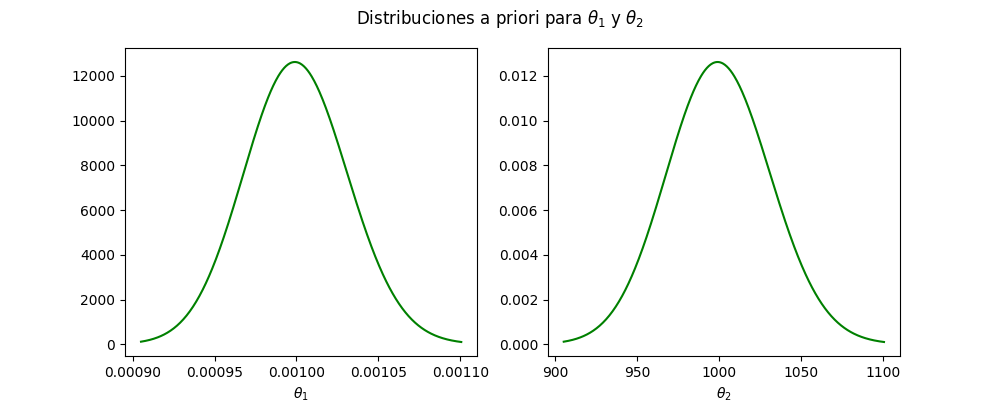
\includegraphics[width = 15 cm]{img/Exp_Central_logistico_sigma/Figuras/Generales/Apriori_logistico_sigma.png}     
    \caption{Distribuciones a priori para $\theta_1$ y $\theta_2$}
    \label{Fig. 3.2.log.priori}
\end{figure} 

De esta forma, análogo al modelo gravitacional, generamos una cadena con la implementación del algoritmo Metropolis-Hastings dado por \cite{christen2010general} con $T = 600,000$ iteraciones y un burn in de 20,000 estados. La distribución posterior, Fig. \ref{Fig. 3.2.log.conjunta}, muestra una forma acampanada ligeramente simétrica con una sutil correlación negativa entre parámetros. Las distribución marginal para $\theta_1$ y $\theta_2$ se muestran en la Fig. \ref{Fig. 3.2.log.theta1} y \ref{Fig. 3.2.log.theta2}.

\begin{figure}
    \centering 
    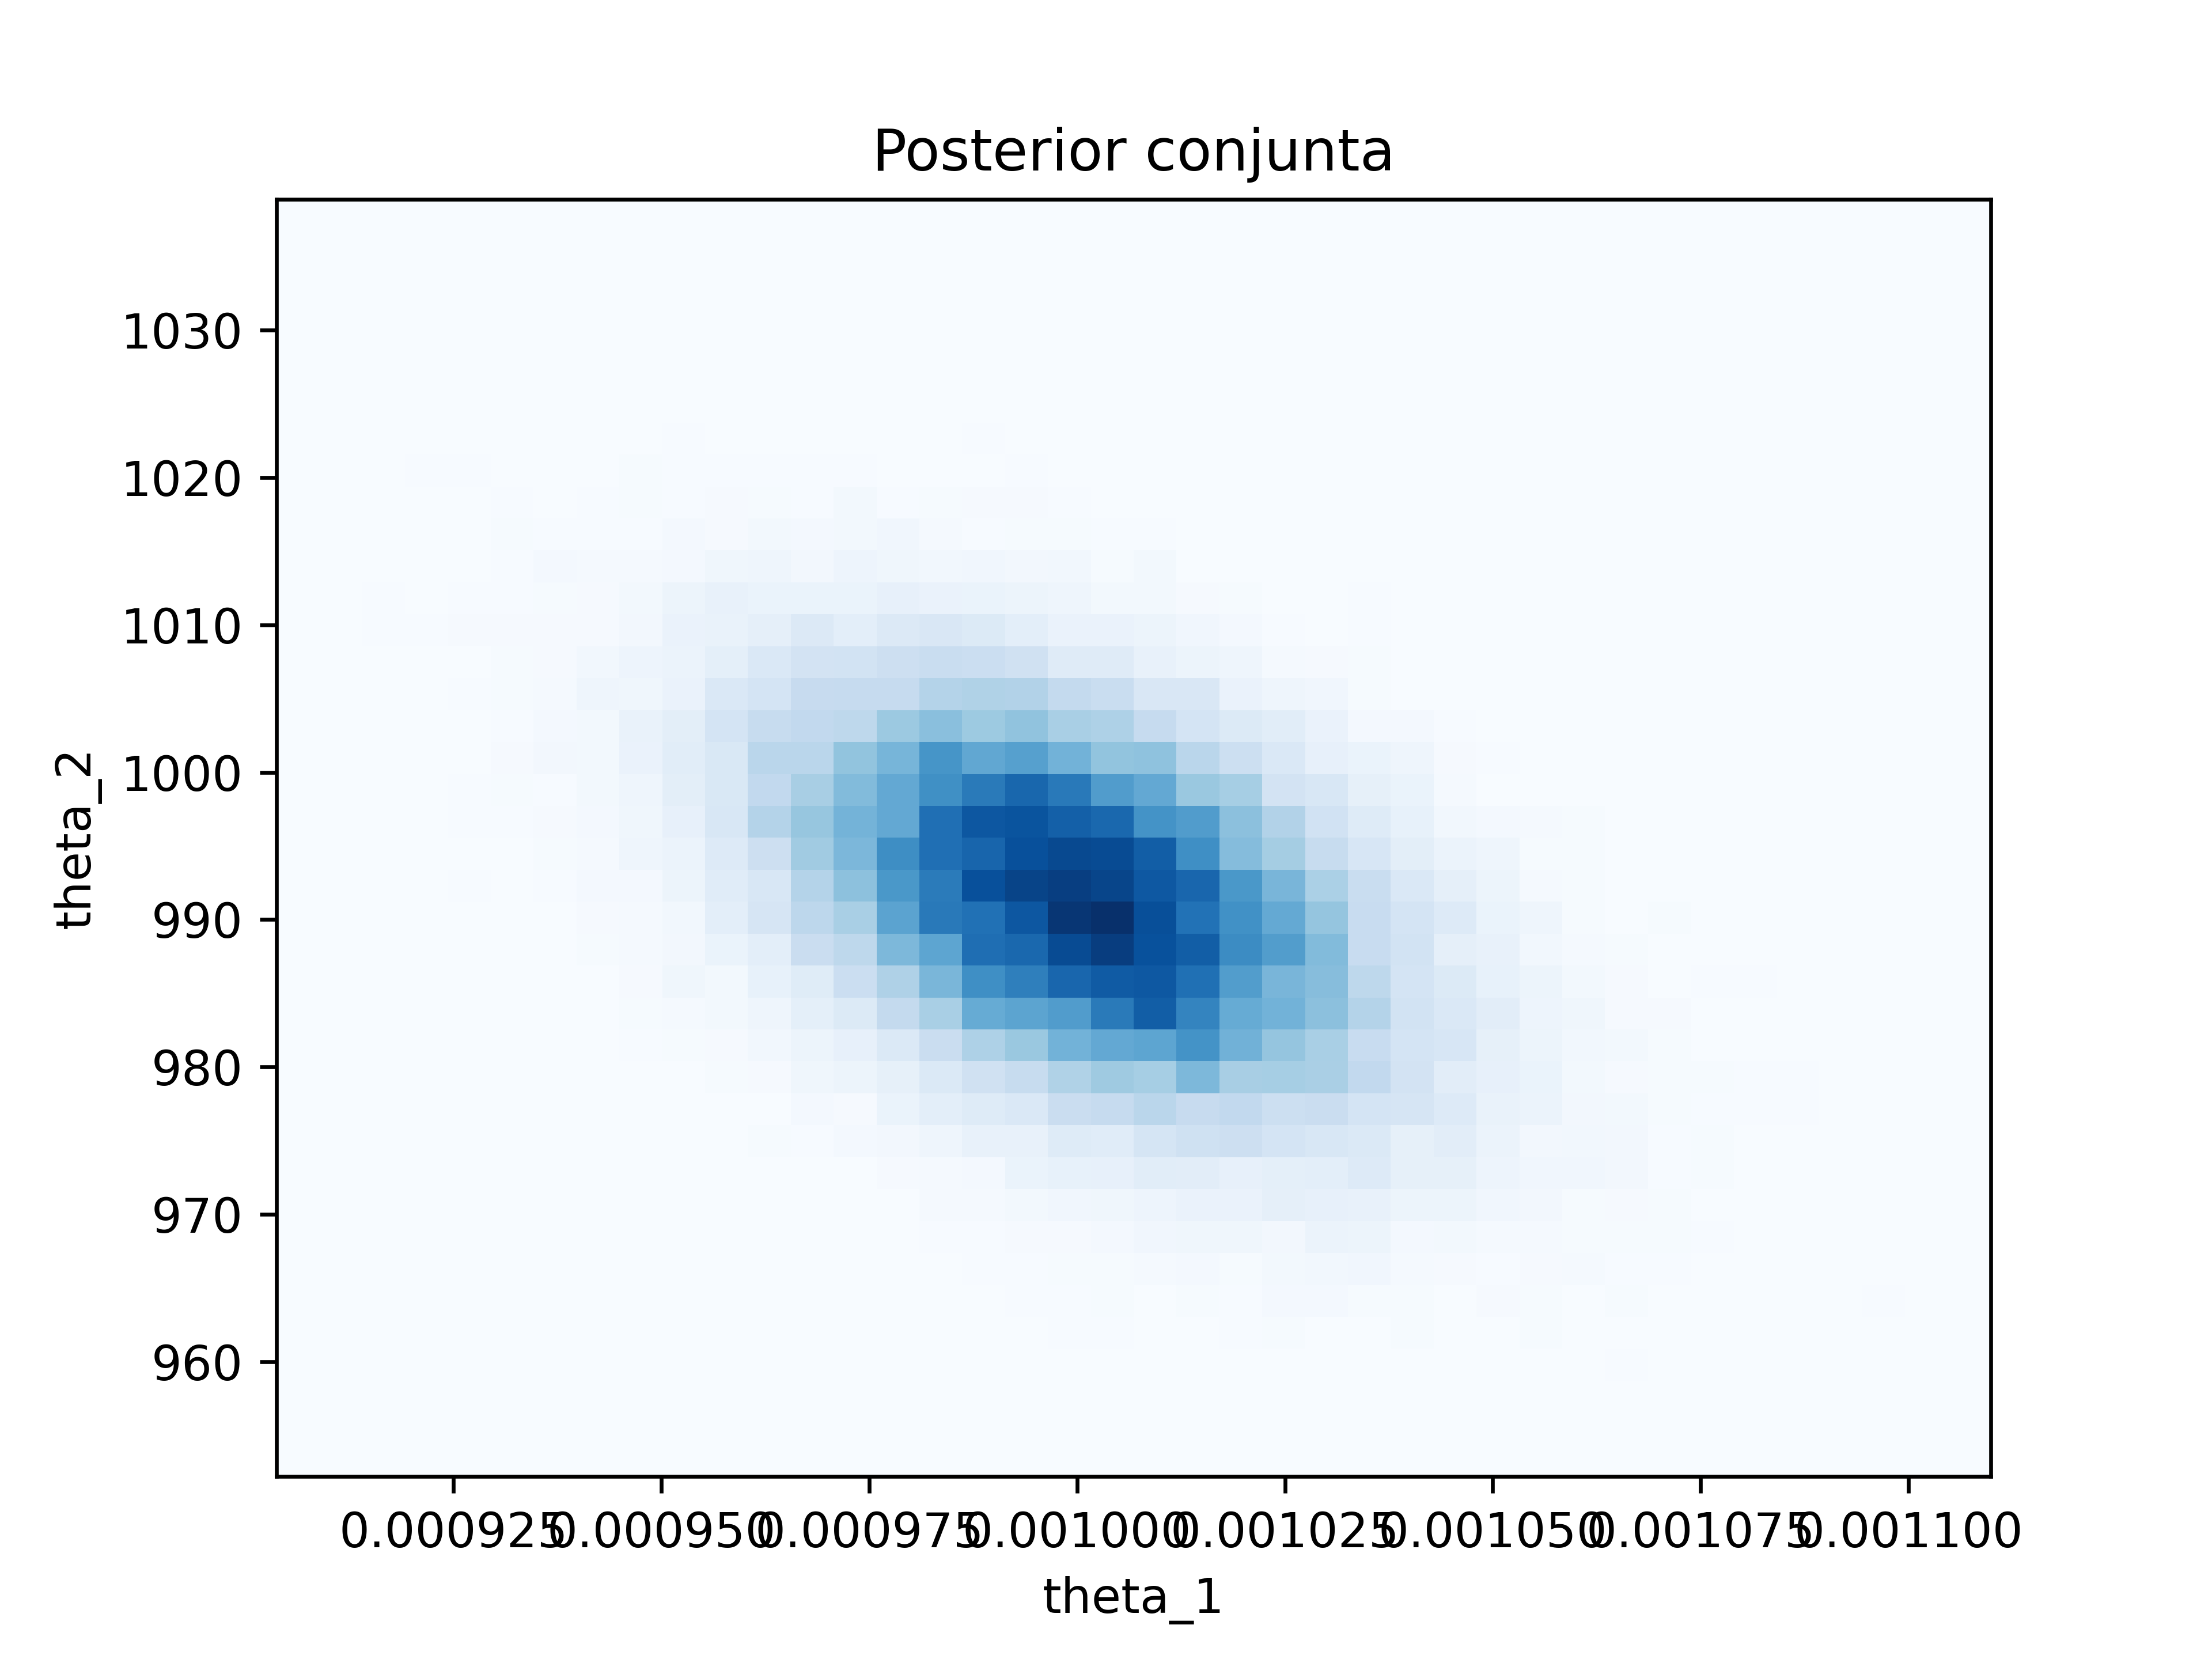
\includegraphics[width = 10 cm ]{img/Exp_Central_logistico_sigma/Figuras/Generales/Conjunta_logistico_sigma.png} 
    \caption{Posterior conjunta para el modelo logístico.}
    \label{Fig. 3.2.log.conjunta}
\end{figure} 

\begin{figure}
    \centering
    \subfloat[Subfigure 1 list of figures text][Posterior para $\theta_1$.]{
    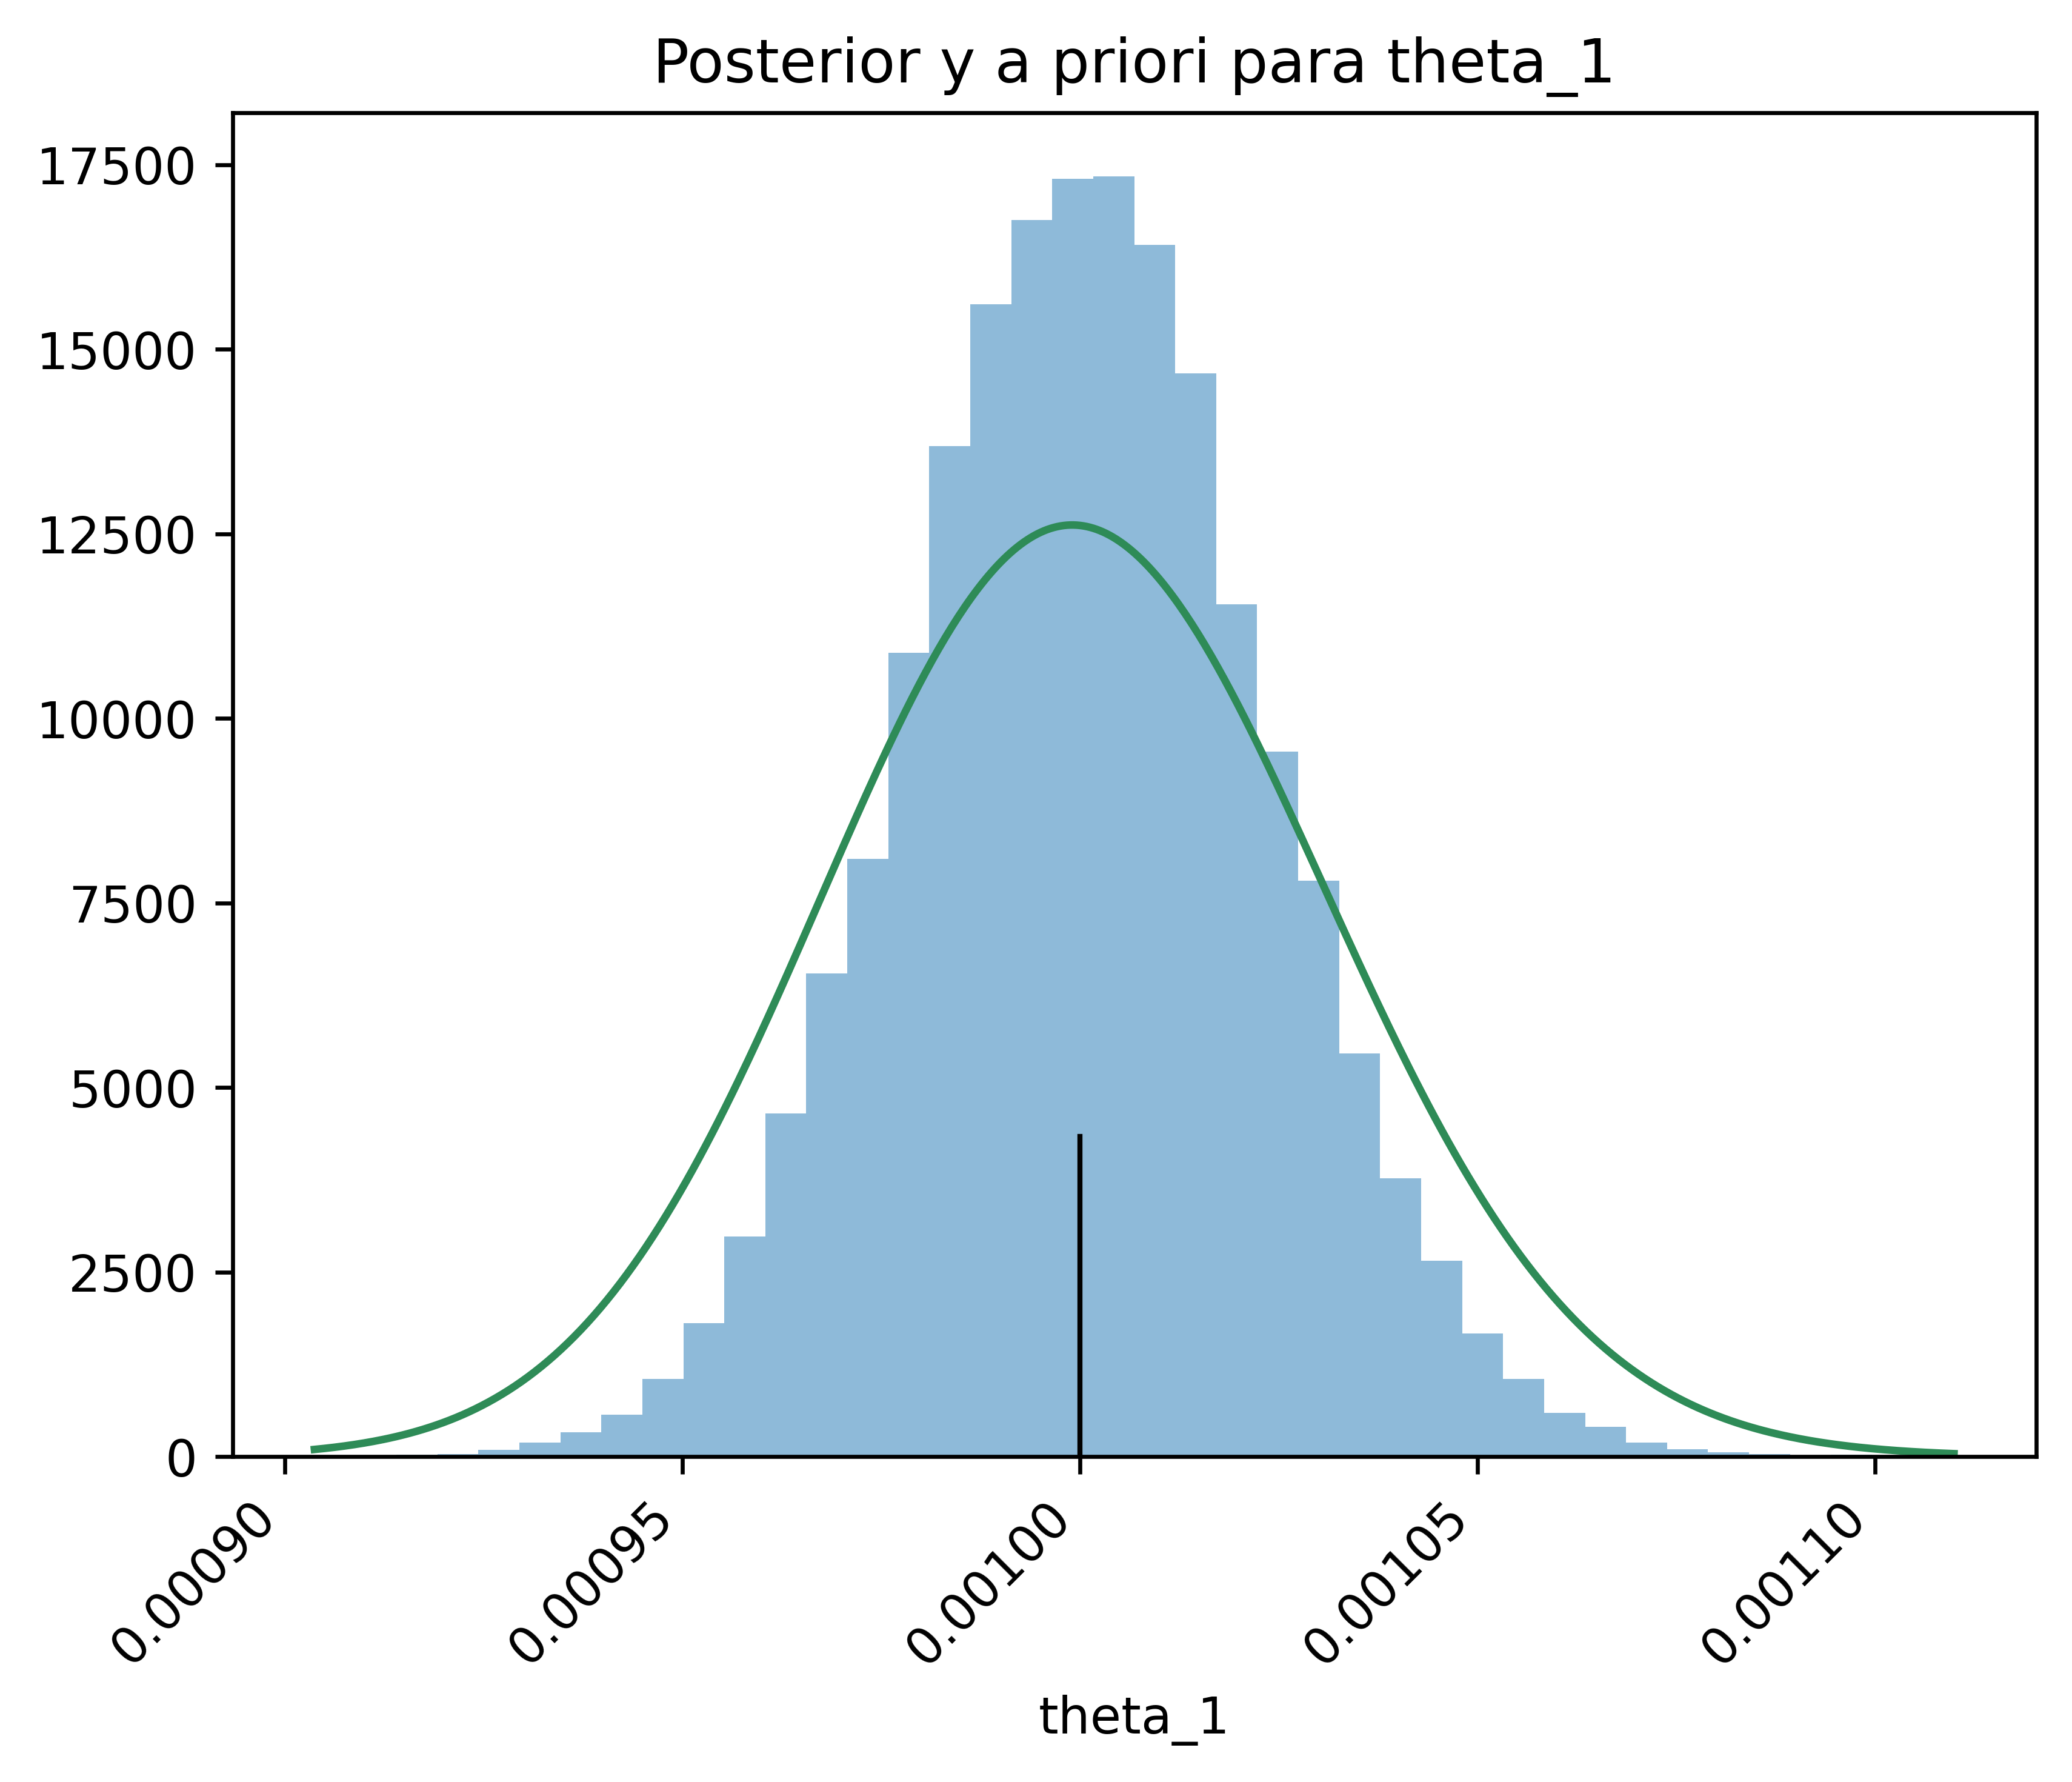
\includegraphics[width=0.4\textwidth]{img/Exp_Central_logistico_sigma/Figuras/Generales/Post_theta1_logistico_sigma.png}
    \label{Fig. 3.2.log.theta1}}
    \qquad
    \subfloat[Subfigure 2 list of figures text][Posterior para $\theta_2$.]{
    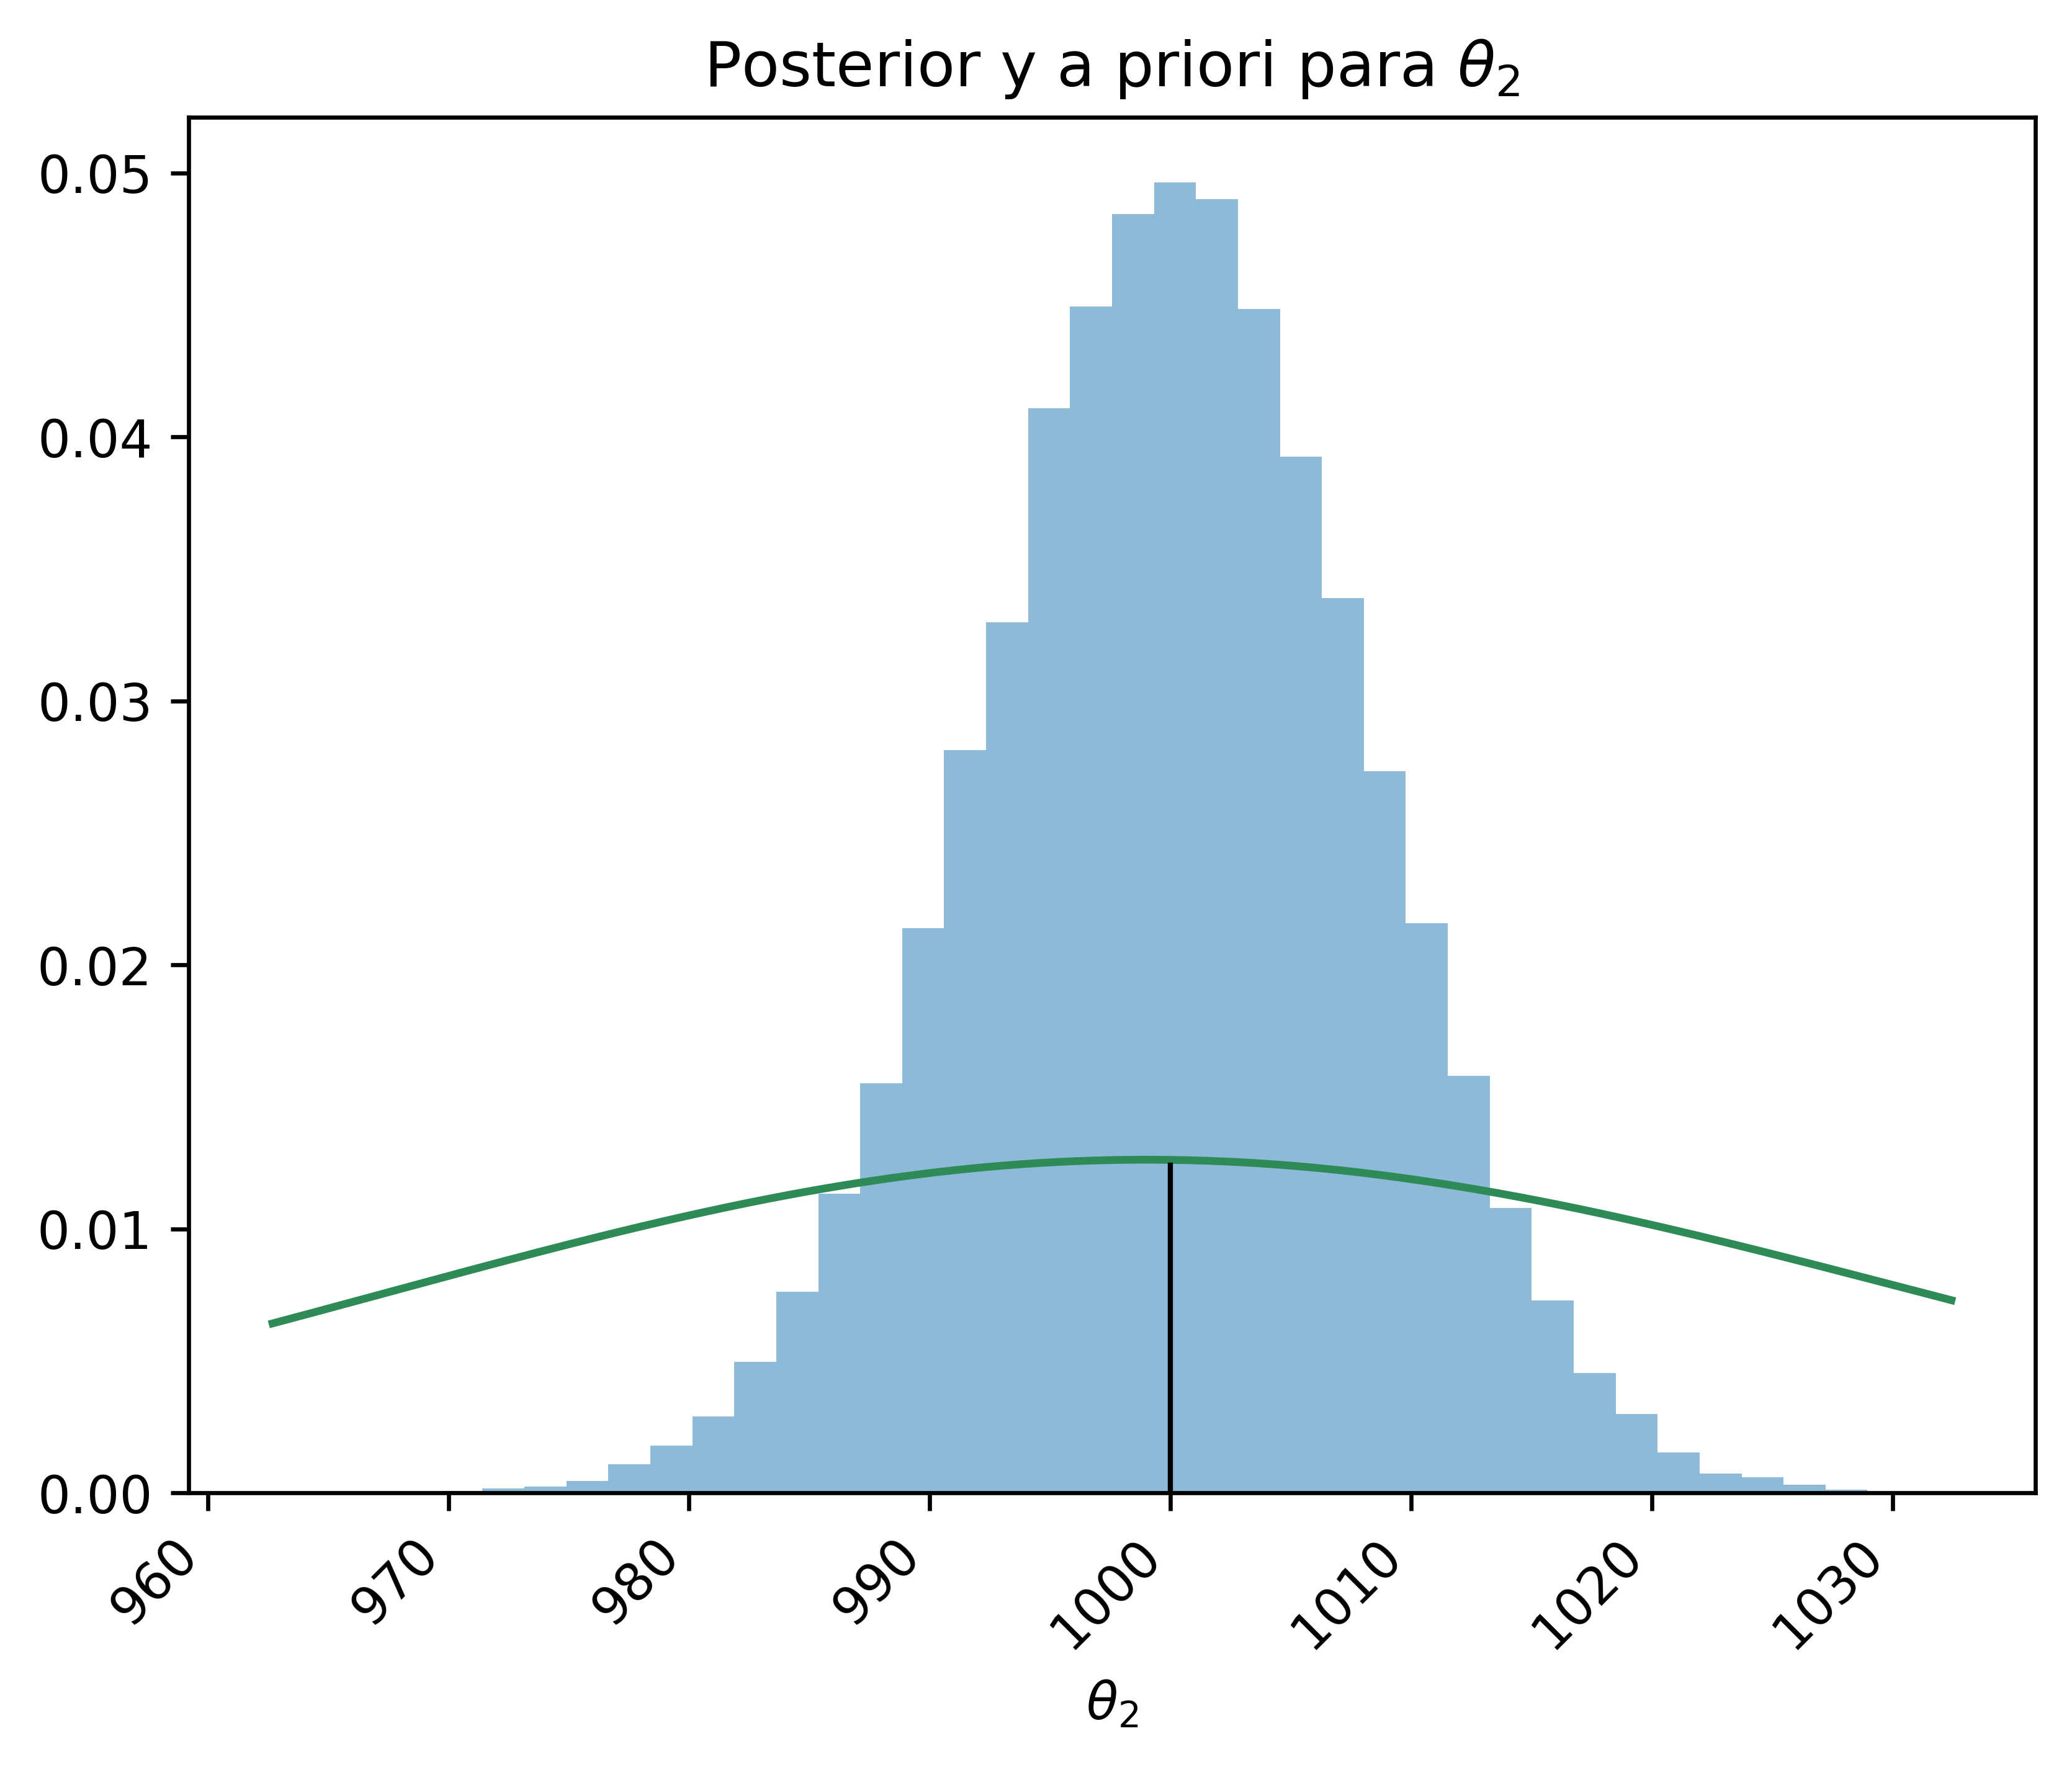
\includegraphics[width=0.4\textwidth]{img/Exp_Central_logistico_sigma/Figuras/Generales/Post_theta2_logistico_sigma.png}
    \label{Fig. 3.2.log.theta2}}
    \caption{Distribución posterior (azul) y distribución a priori (verde) para el parámetros $\theta_1$ y $\theta_2$ del modelo logístico.}
    \label{Fig. 3.2.log.theta}
\end{figure}

Finalmente, el análisis concluye con la distribución predictiva dada por el forward map tomando estimaciones puntuales de la distribución posterior, en la Fig. \ref{Fig. 3.2.log.predictiva} notamos que la distribución tiene una varianza mayor que en el modelo gravitacional, además de observar que la trayectoria de partida (azul oscuro) se encuentra incluida en la predicción dada por el problema inverso.

\begin{figure}
    \centering 
    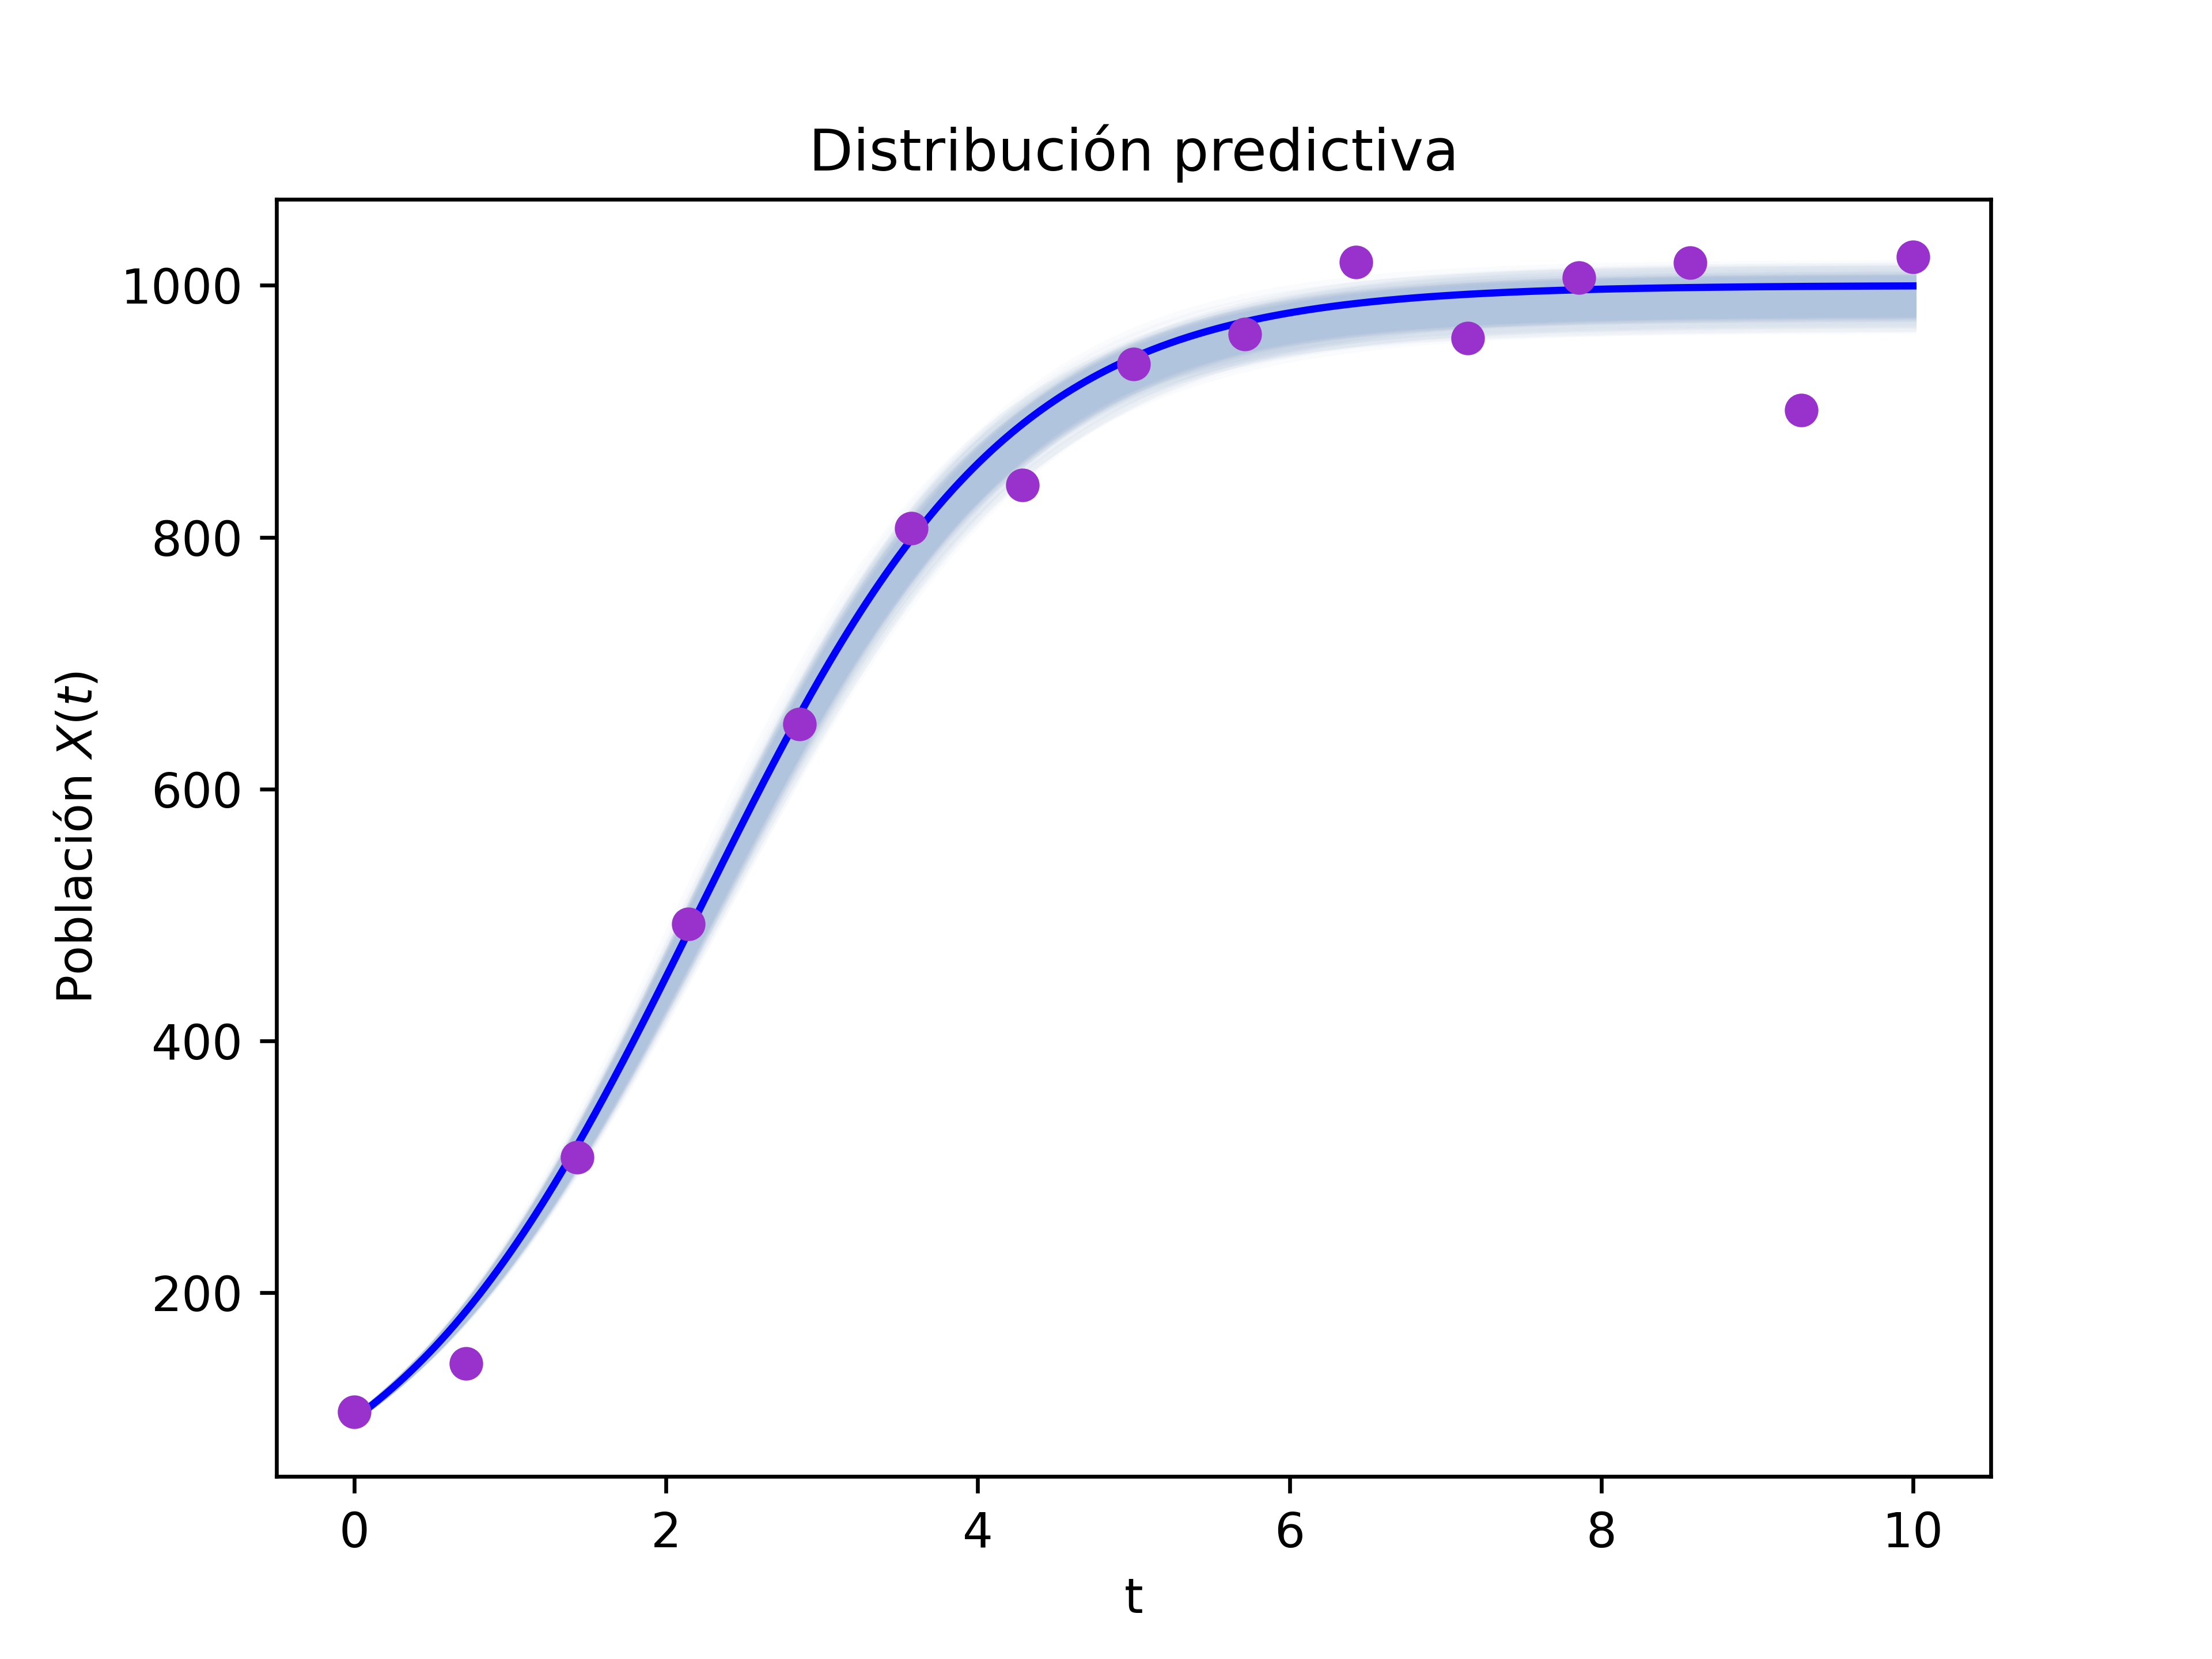
\includegraphics[width = 10 cm ]{img/Exp_Central_logistico_sigma/Figuras/Generales/Predictiva_logistico_sigma.png} 
    \caption{Distribución predictiva para el modelo logístico.}
    \label{Fig. 3.2.log.predictiva}
\end{figure} 

\subsubsection{Simulación del modelo SIR}

Para el modelo epidemiólogico tomamos una muestra de $n =10$ observaciones de infectados en una población cerrada a lo largo del tiempo. Al igual que los modelos previos, dichas observaciones son simulaciones del forward map con ruido gaussiano. En la Fig. \ref{Fig. SIR_01} vemos la grafica de la muestra de infectados, notamos que tienen un rápido crecimiento para después decaer suavemente.

\begin{figure}
    \centering 
    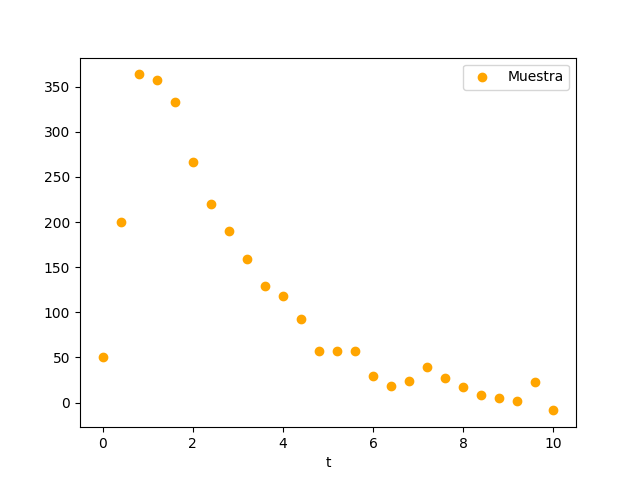
\includegraphics[width = 10 cm]{img/Exp_Central_SIR_sigma/Figuras/Generales/Muestra_SIR_sigma.png} 
    \caption{Muestra $\mathbf{y}$ del modelo SIR.}
    \label{Fig. SIR_01}
\end{figure} 

Para abordar el problema inverso establezcamos los parámetros que se desea hacer inferencia. El espacio parametral se conforma por $\theta = (\beta,\gamma)$ donde $\beta >0$ es la tasa de infección y $\gamma > 0$ es la tasa de recuperación dados en (\ref{3.1.3.01}). Nuevamente como se trata de parámetros positivos usamos la distribución a priori (\ref{3.2.1.03}). Podemos rescatar un conocimiento a priori sobre su distribución previo a los datos (\cite{weiss2013sir}). La elección considera para las distribuciones gamma a priori son mostradas en la Fig. \ref{Fig. SIR_02}.

\begin{figure}[H] 
    \centering 
    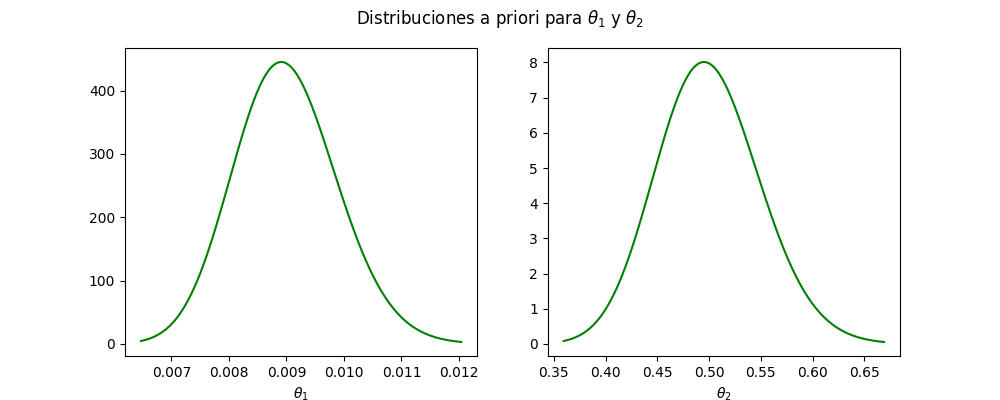
\includegraphics[width = 15 cm ]{img/Exp_Central_SIR_sigma/Figuras/Generales/Apriori_SIR_sigma.png} 
    \caption{Distribuciones marginal a priori para el parámetro $\beta$ (izquierda) y $\gamma$ (derecha).}
    \label{Fig. SIR_02}
\end{figure} 

Análogamente a los modelos previos, una vez obtenida la forma funcional de la distribución posterior, usando el algoritmo Metropolis-Hastings para una cadena de tamaño $T = 600,000$. La distribución posterior dada se muestra en la Fig. \ref{Fig. SIR_03} que muestra una forma de media luna concentrada en el borde izquierdo. 

\begin{figure}[H] 
    \centering 
    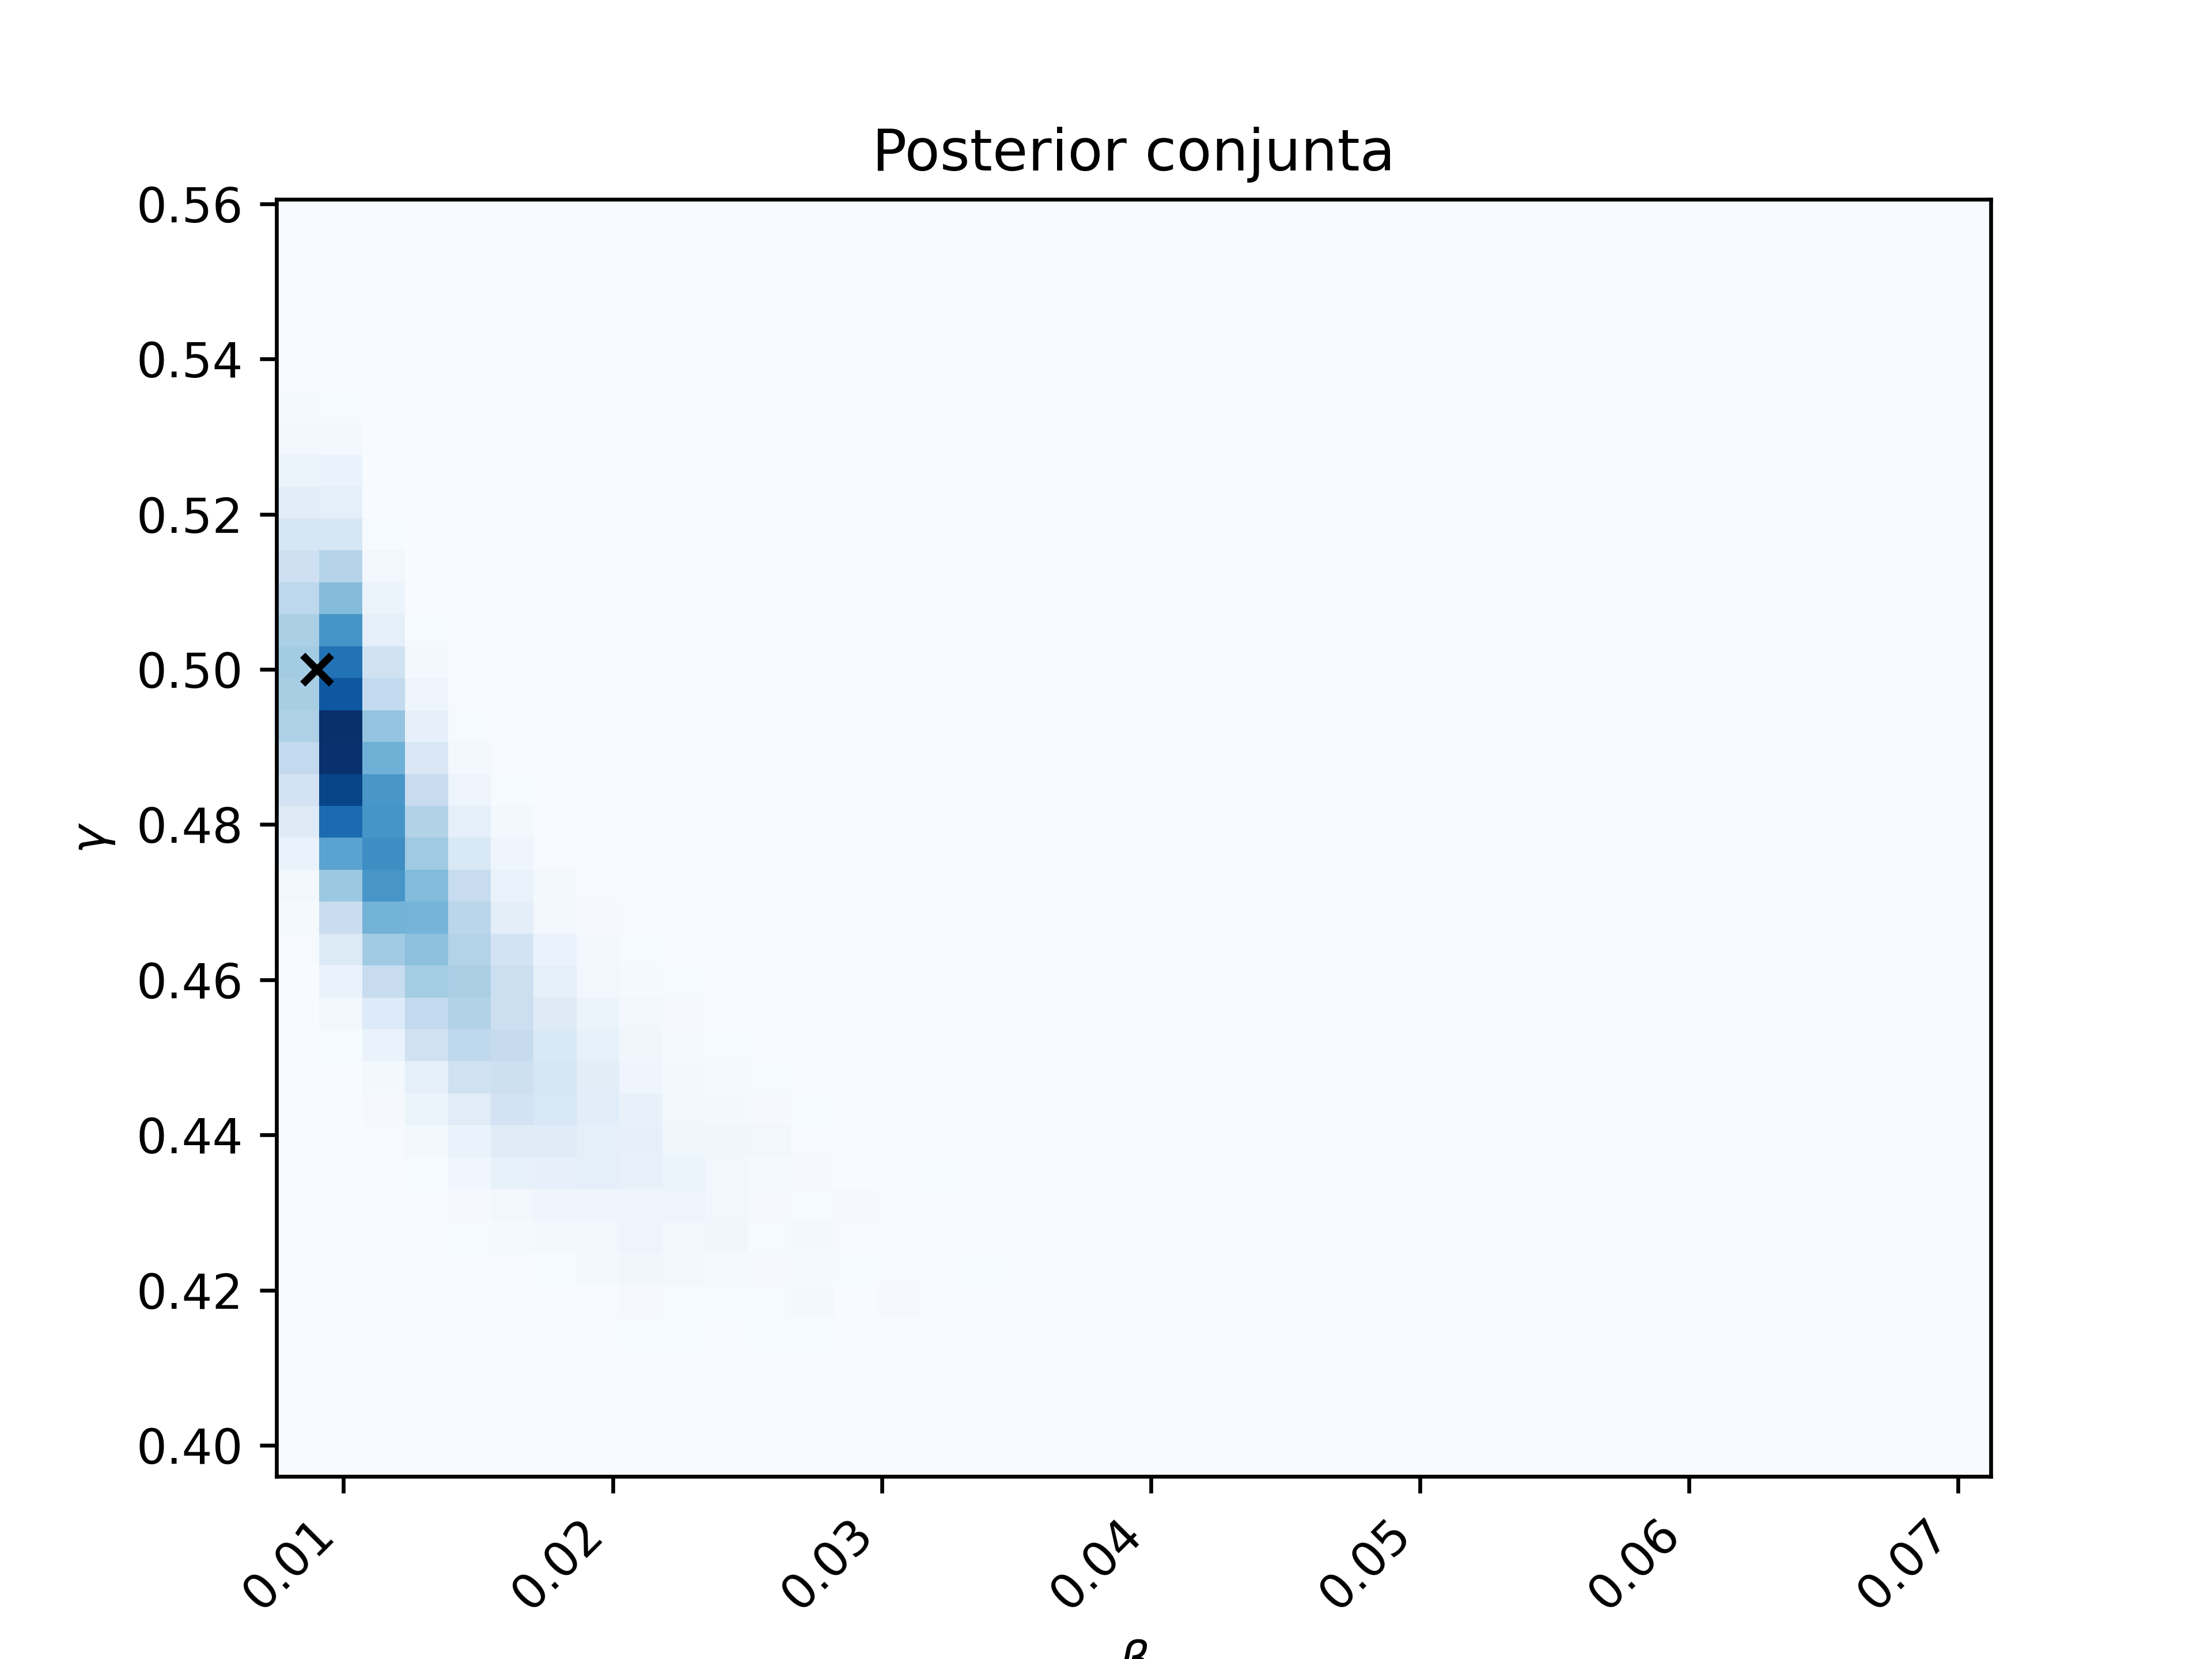
\includegraphics[width = 10 cm]{img/Exp_Central_SIR_sigma/Figuras/Generales/Conjunta_SIR_sigma.png} 
    \caption{Distribución posterior conjunta para el modelo SIR.}
    \label{Fig. SIR_03}
\end{figure} 

\begin{figure}[h]
    \centering
    \subfloat[Subfigure 1 list of figures text][Posterior para $\beta$.]{
    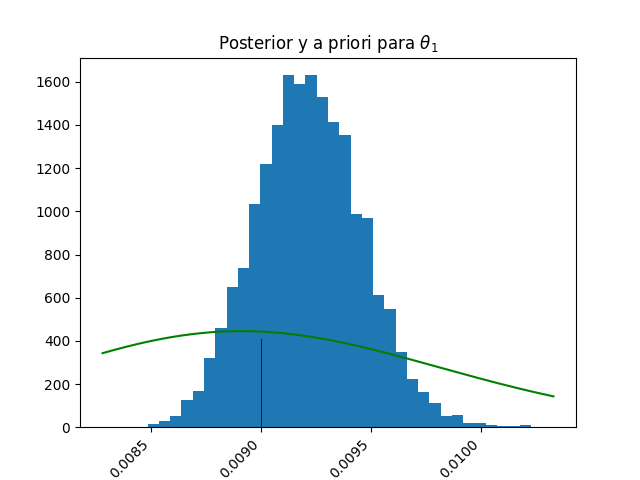
\includegraphics[width=0.4\textwidth]{img/Exp_Central_SIR_sigma/Figuras/Generales/Post_theta1_SIR_sigma.png}
    \label{Fig. SIR_04}}
    \qquad
    \subfloat[Subfigure 2 list of figures text][Posterior para $\gamma$.]{
    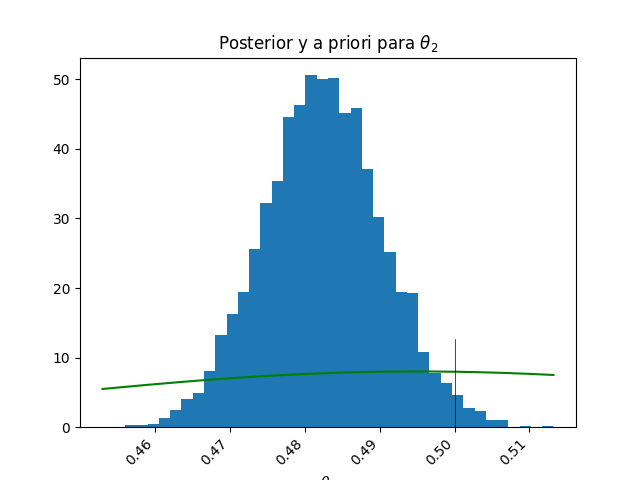
\includegraphics[width=0.4\textwidth]{img/Exp_Central_SIR_sigma/Figuras/Generales/Post_theta2_SIR_sigma.png}
    \label{Fig. SIR_05}}
    \caption{Distribución posterior (azul) y distribución a priori (verde) para el parámetros $\beta$ y $\gamma$ del modelo SIR. }
    \label{Fig. SIR.theta}
\end{figure}

Para observar la distribución para cada parámetro se toma la distribución marginal, respectivamente. Observemos de la Fig. \ref{Fig. SIR_04} y Fig. \ref{Fig. SIR_05} la distribución de $\beta$ se aglomera en valores cercanos a cero, mientras que para $\gamma$ tenemos bastante diferencia respecto a la distribución a priori.

Tomando realizaciones $ \theta_j = (\beta_j,\gamma_j)$ de la distribución posterior para luego calcular $F(\theta_j)$ nos da la distribución vista para la cantidad de infectados en tiempo arbitrario dado por el modelo SIR. Tal gráfico dado en Fig. \ref{Fig. SIR_06} vemos que el modelo (azul fuerte) se encuentra incluido en las distribuciones de infectados.

\begin{figure}[H] 
    \centering 
    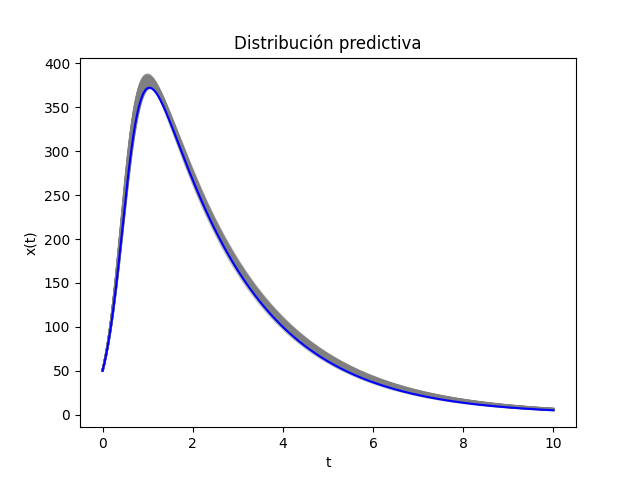
\includegraphics[width = 10 cm ]{img/Exp_Central_SIR_sigma/Figuras/Generales/Predictiva_SIR_sigma.png} 
    \caption{Distribución predictiva para el modelo SIR.}
    \label{Fig. SIR_06}
\end{figure} 


\section{Simulación con forward map aproximado}

% % \subsection{Experimentación con la convergencia.}

% % En esta sección se abordan las diferentes simulaciones para cada modelo. Empezando por el modelo de gravedad sujeto a fricción, nos interesa la distribución posterior de los parámetros $g$ y $b$. Con la metodología establecida y usando MCMC con la a priori \textcolor{red}{Grafico de la priori} anteriormente mencionada obtenemos una simulación de la distribución posterior conjunta. Tomando la marginal de cada parámetro y haciendo el histograma para la estimación de la distribución marginal tenemos las siguientes distribuciones posteriores marginales.


% % \textcolor{red}{Poner la distribución posterior marginal con Forward ordinario}

% % Consideremos ahora la distribución posterior conjunta obtenida con el Forward map aproximado. En este caso, se hace el experimento para la cantidad de 5,8,16 vecinos cercanos y a su vez cada uno de ello haciendo la malla cada vez más fina. Para cada Forward con la cantidad dada de vecinos cercanos se propone una malla en el espacio de parámetros $(g,b)\in \Theta$ de tamaño 10x10, 15x15, 30x30, 50x50.

% % La muestra inicial de la trayectoria que sigue el modelo se hace mediante simulación desde la misma ecuación diferencial dada por el modelo. Es de nuestra elección la cantidad de muestra $n$ que queremos para la distribución posterior conjunta de los parámetros. Sin embargo, para dicha simulación es necesario fijar dos parámetros, que llamaremos parámetros verdadero y obtener la trayectoria $x_t|\theta$. 

% % Para la simulación de los datos consideramos una muestra de 30 datos del modelo de gravedad en el intervalo de tiempo $[0,1.5]$. 

% % Las distribuciones posteriores marginales de $g$ se muestran en las figuras \ref{fig:g_01} \ref{fig:g_02}    \ref{fig:g_03} 


% Con la propuesta aproximada para el análisis bayesiano para el problema inverso que resulta ser bastante conveniente dado que ya hemos visto que la metodología desarrollada que la distribución posterior depende del forward map (ordinario), y por ello el algoritmo de Metropolis-Hastings requiere que a cada paso en el espacio de estados $\Theta$ en la cadena $X_t$, se solucione la ecuación diferencial del modelo para los parámetros propuestos por MCMC. Sin embargo, tenemos cadenas de medio millón de pasos, lo que complica el análisis bayesiano. Por tanto, tenemos que el análisis aproximado ahorra tiempo de computo al evitar calcular el forward map iterativamente.

% % \subsection{Regla de interpolación(aproximación de forward map)}
% Con la regla de interpolación dada en (\textcolor{red}{referencia}) aproximamos el forward map repetidamente. Se pretende buscar la mejor aproximación a la distribución posterior modificando el forward aproximado tanto en la cantidad de puntos por rejilla así con en la cantidad de vecinos cercanos contemplados para la interpolación. 

% Las aproximaciones del forward map se hacen con inferencias de los k puntos más cercanos. Particularmente se experimentó con vecinos $k = 3,5,8$. Además, para la densidad de puntos de la rejilla, se toman sucesivamente rejillas de tamaño $m \text{x} m$ con $m = 10, 15, 30, 50$.

% \textcolor{blue}{Imagen discretización forward map}



% \subsection{Método aproximado al problema inverso}
% \subsubsection{Forward map aproximado para el modelo gravitatorio}

% En el análisis bayesiano sobre el modelo gravitatorio se obtuvo la distribución posterior con el forward map ordinario para cada una de las aproximaciones propuestas. 

% Tomemos la aproximación del forward map con 3 vecinos cercanos $(k= 3)$. Luego, calculemos la distribución posterior para cada rejilla $(m = 10, 15, 30, 50)$. Tenemos la distribución bidimensional conjunta. Luego se toma las distribuciones marginales para cada parámetro $g,b$. Al ser un estudio heurístico, el grado de aproximación se hace tras simple comparación de la distribución marginal aproximada  para cada parámetro, $\pi^{*}(g)$ con $\pi(g)$, y comparación de $\pi^{*}(b) = \pi(b)$.


% En la Fig. () se muestran las distribuciones marginales para la aproximación del forward map con $k = 3$ y de izquierda a derecha una malla de 10x10, 15x15, 30x30, 50x50.

% \begin{figure}[H] 
%     \centering 
%     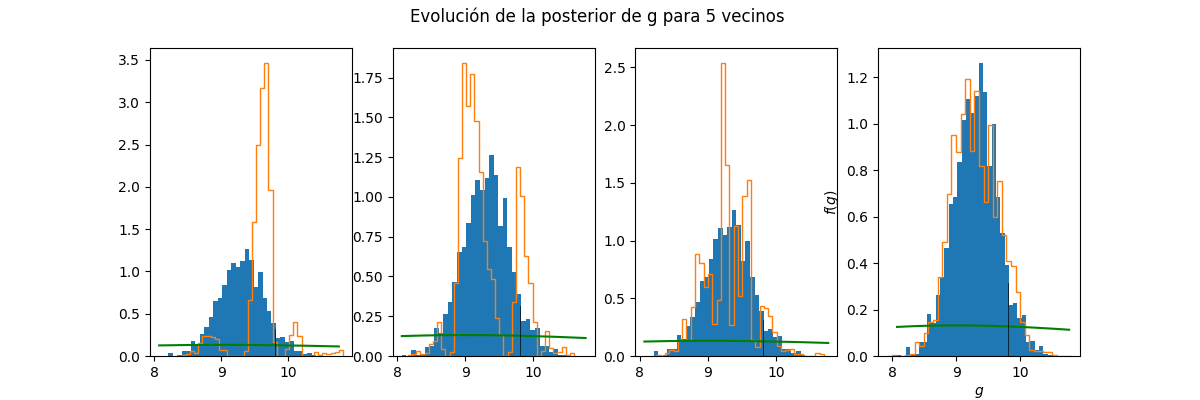
\includegraphics[width = 16 cm ]{img/Exp_Central_gravedad_Sigma/Figuras/Generales/Convergencia_theta1_1_gravedad_sigma.png} 
%     % \caption{}
%     % \label{Fig. }
% \end{figure} 

% \begin{figure}[H] 
%     \centering 
%     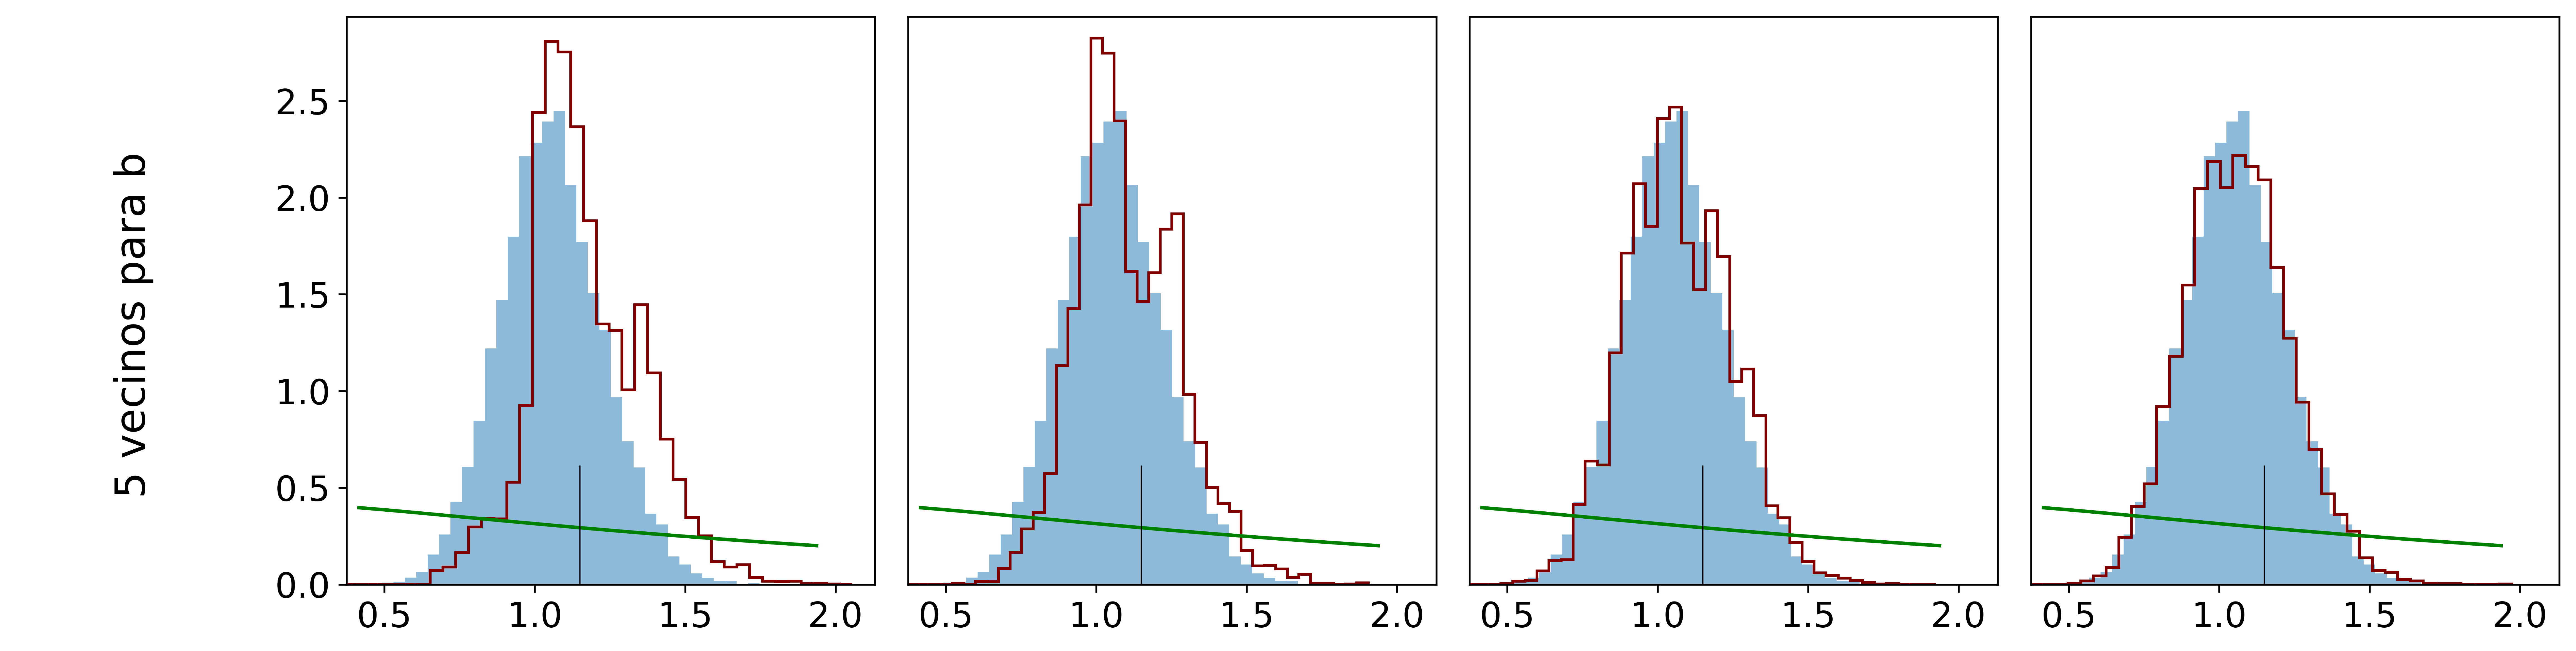
\includegraphics[width = 16 cm ]{img/Exp_Central_gravedad_Sigma/Figuras/Generales/Convergencia_theta2_1_gravedad_sigma.png} 
%     % \caption{}
%     % \label{Fig. }
% \end{figure} 

% En la Fig. () se muestran las distribuciones marginales para la aproximación del forward map con $k = 5$ y de izquierda a derecha una malla de 10x10, 15x15, 30x30, 50x50.

% \begin{figure}[H] 
%     \centering 
%     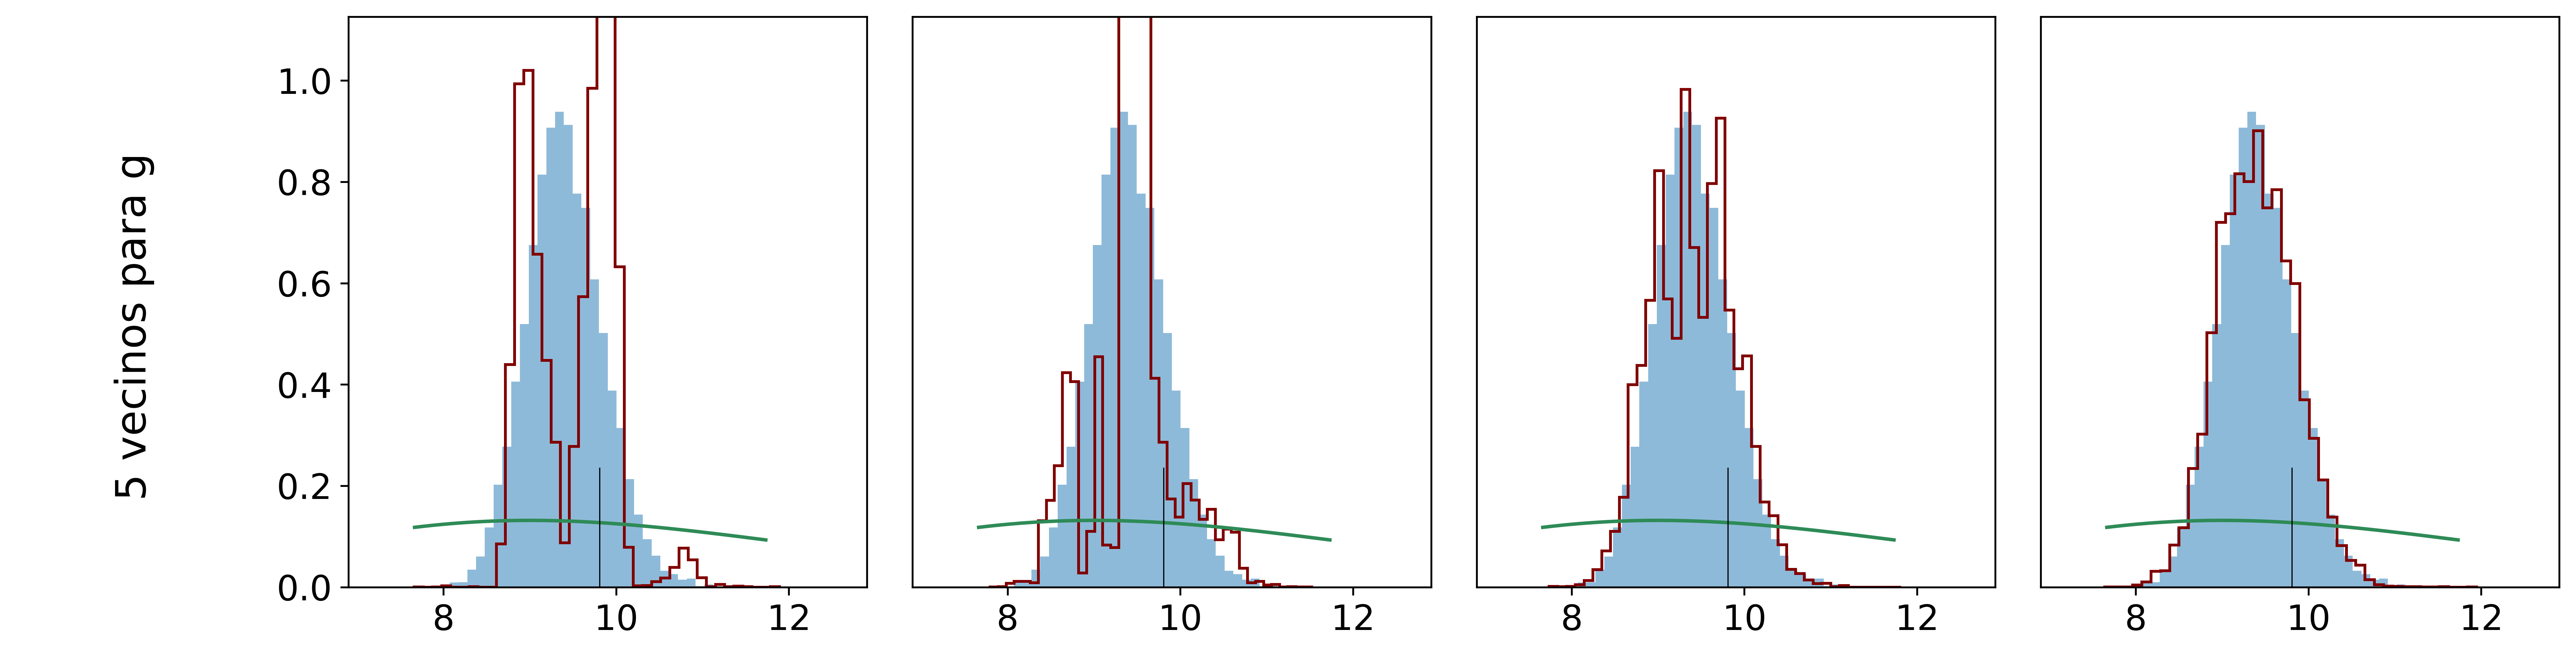
\includegraphics[width = 16 cm ]{img/Exp_Central_gravedad_Sigma/Figuras/Generales/Convergencia_theta1_2_gravedad_sigma.png} 
%     % \caption{}
%     % \label{Fig. }
% \end{figure} 

% \begin{figure}[H] 
%     \centering 
%     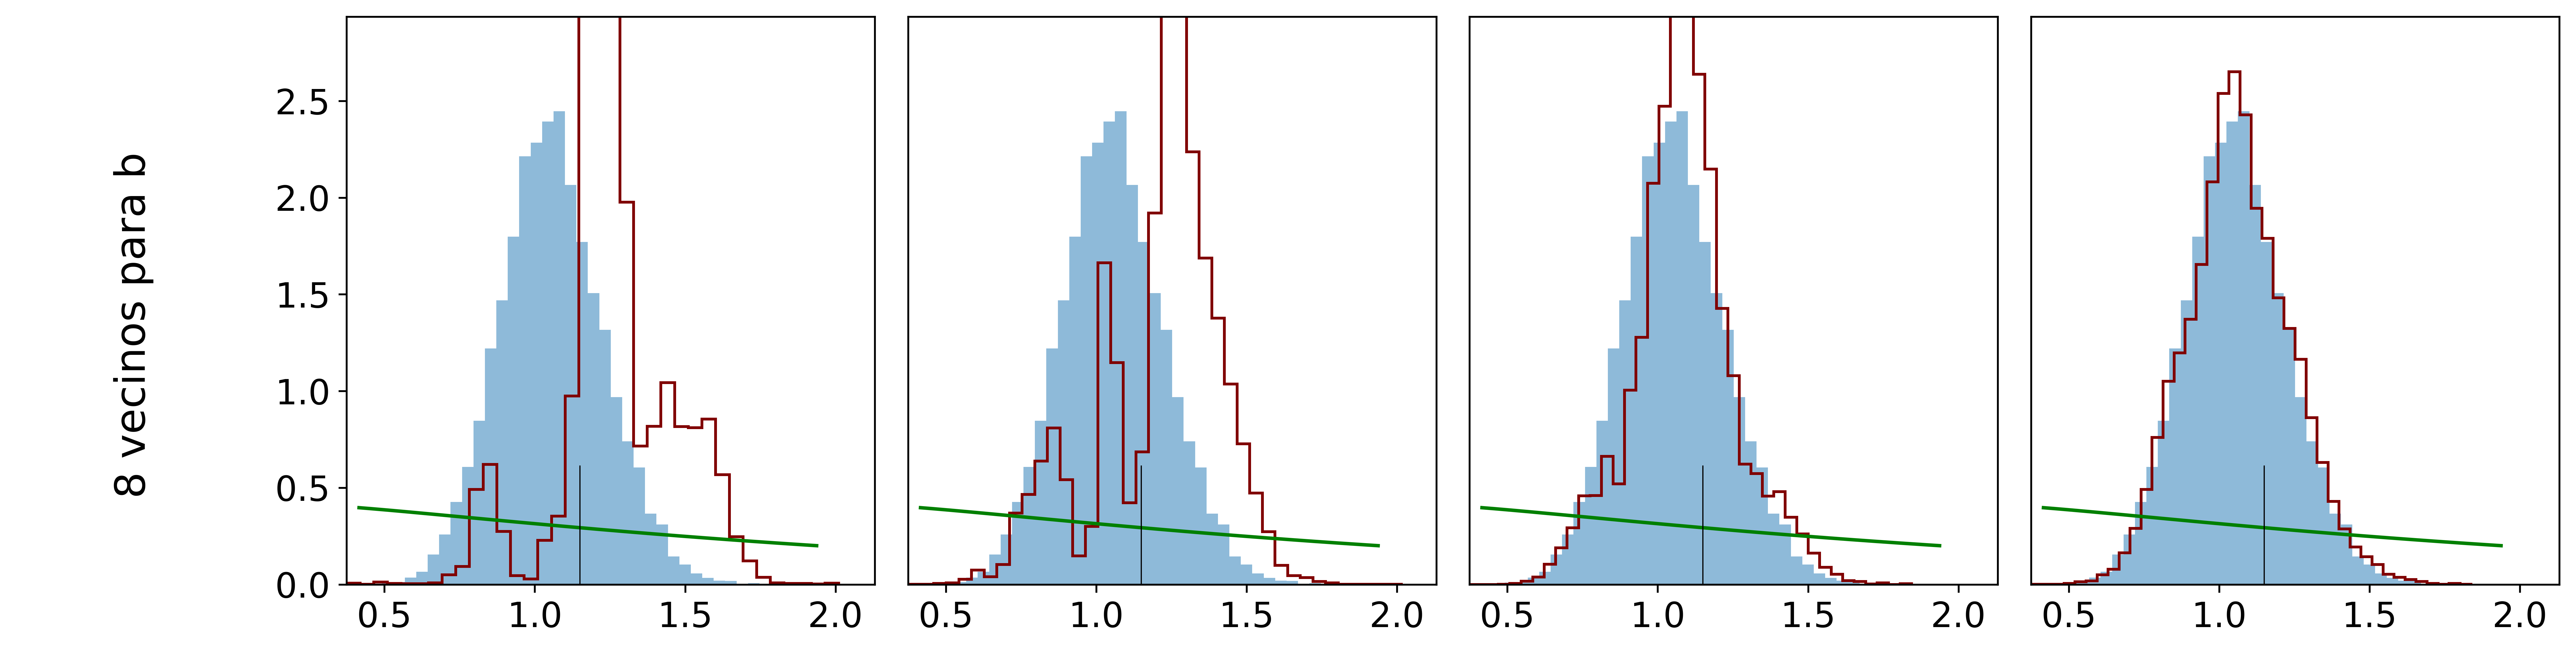
\includegraphics[width = 16 cm ]{img/Exp_Central_gravedad_Sigma/Figuras/Generales/Convergencia_theta2_2_gravedad_sigma.png} 
%     % \caption{}
%     % \label{Fig. }
% \end{figure} 

% En la Fig. () se muestran las distribuciones marginales para la aproximación del forward map con $k = 8$ y de izquierda a derecha una malla de 10x10, 15x15, 30x30, 50x50.

% \begin{figure}[H] 
%     \centering 
%     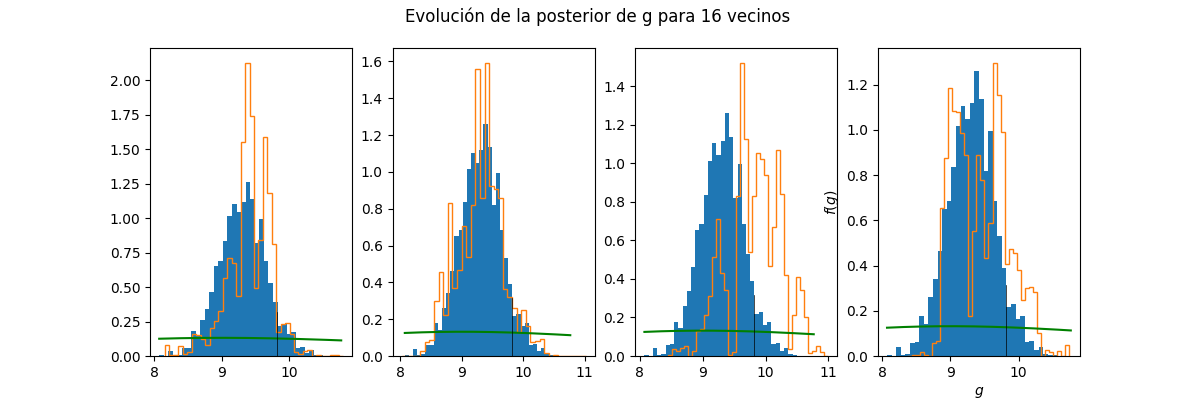
\includegraphics[width = 16 cm ]{img/Exp_Central_gravedad_Sigma/Figuras/Generales/Convergencia_theta1_3_gravedad_sigma.png} 
%     % \caption{}
%     % \label{Fig. }
% \end{figure} 

% \begin{figure}[H] 
%     \centering 
%     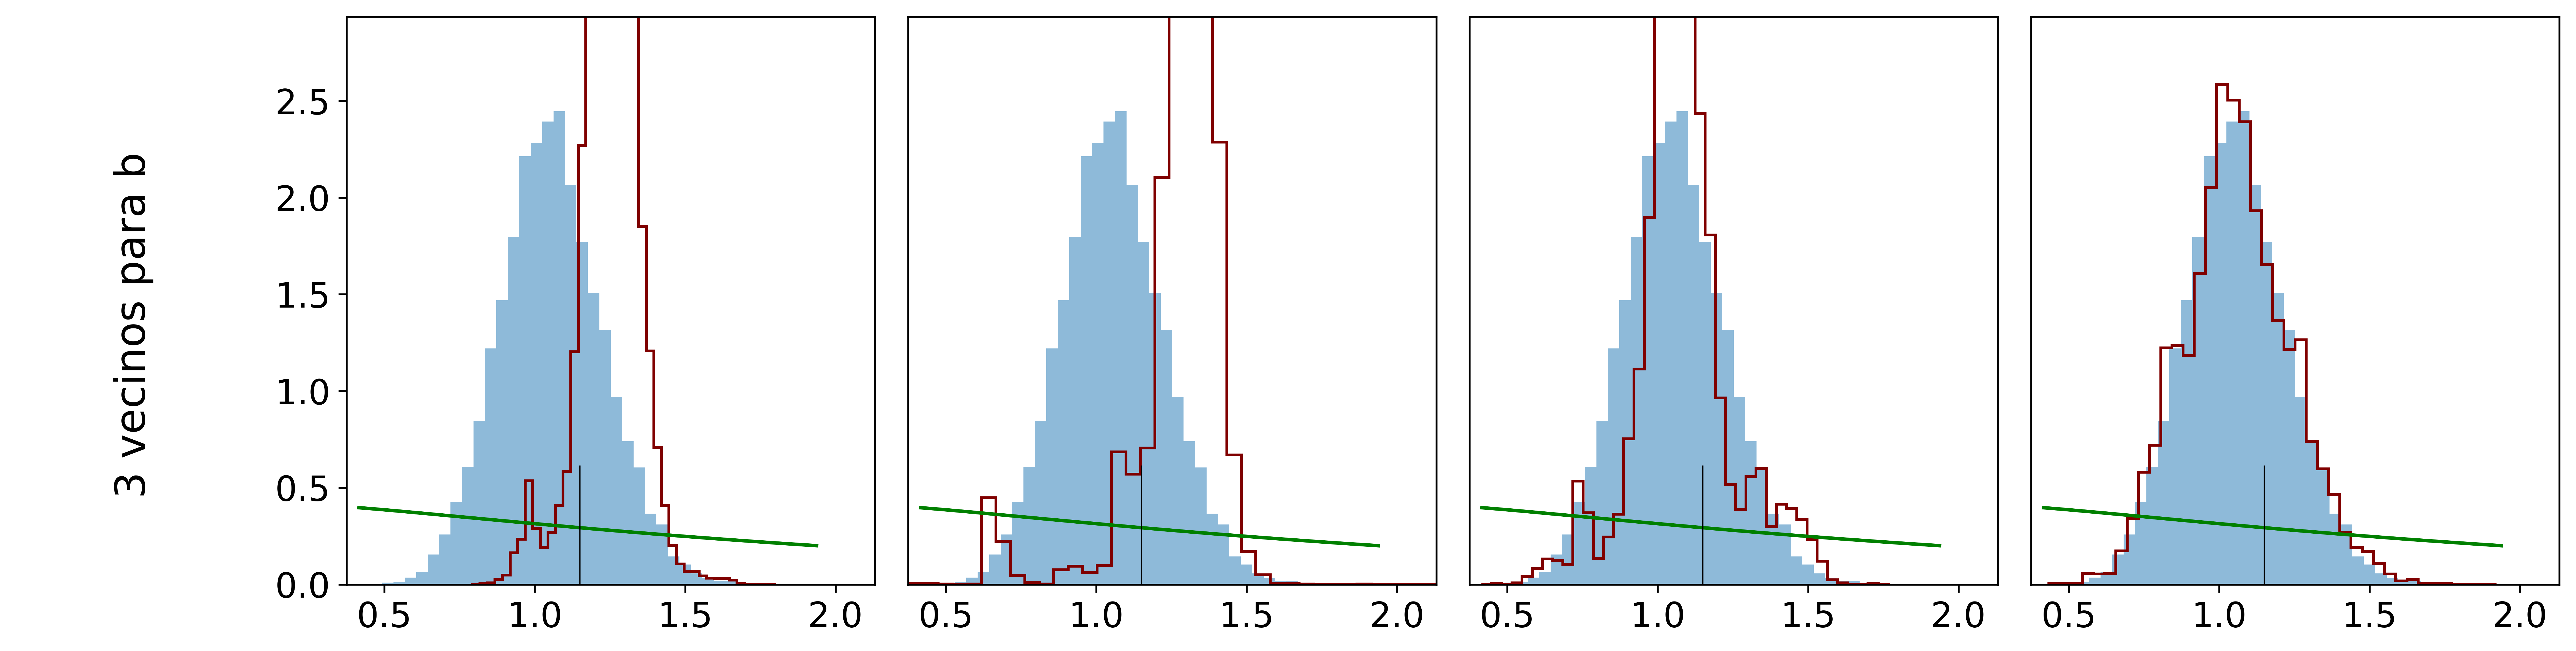
\includegraphics[width = 16 cm ]{img/Exp_Central_gravedad_Sigma/Figuras/Generales/Convergencia_theta2_3_gravedad_sigma.png} 
%     % \caption{}
%     % \label{Fig. }
% \end{figure} 

% Notemos del análisis previo que de manera general las distribuciones posteriores aproximadas $\pi^{*}(g,b)$ mejora a medida que la malla se hace más fina. Luego, la mejor aproximación se obtiene con la malla más fina que discretiza el espacio parametral en 50x50 puntos. Queda definir que cantidad de vecinos hace la aproximación mejor. Notese que para 8 vecinos (k = 8) no ajusta para el parámetro $g$ lo que descarta esta elección. Finalmente, para 3 y 5 vecinos tenemos distribuciones bastante similares por lo que la elección es indiferente. Así, seleccionamos el forward map aproximado con 3 vecinos en una malla 50x50.

% Es necesario establecer una estructura para realizar comparaciones entre el método ordinario y aproximado. Para saber la factibilidad del método se considera al tiempo de ejecución, que es una variable tangible. 

% El tiempo de ejecución del método ordinario para el problema inverso en el modelo gravitacional es de \textbf{5 min 57 s}


% \begin{table}[H]
%     \centering
%     \begin{tabular}{l r r r c}
%       \toprule
%        \textbf{Malla} & \textbf{\:\:\:\:\:\:\:10 x 10\:\:\:\:\:\:\:} & \textbf{\:\:\:\:\:\:\:15 x 15\:\:\:\:\:\:\:} & \textbf{\:\:\:\:\:\:\:30 x 30\:\:\:\:\:\:\:} & \textbf{\:\:\:\:\:\:\:50 x 50\:\:\:\:\:\:\:} \\
%       \midrule
%       3 vecinos & 4m 52s & 4m 55s & 5m 52s & \textbf{5m 00s}\\
%       5 vecinos & 5m 03s & 5m 02s & 4m 53s & 5m 02s\\
%       8 vecinos & 5m 00s & 5m 09s & 5m 02s & 5m 02s\\
%       \bottomrule
%     \end{tabular}
%     % \caption{A table caption.}
%     % \label{tabla_03}
% \end{table}

% Vemos que la aproximación elegida tiene una ganancia de 57 segundos de ejecución, lo que representa una ganancia de una sexta parte del tiempo.



% % \begin{figure}[h]
% %     \centering
% %     \subfloat[Subfigure 1 list of figures text][Posterior con Forward aproximado en malla de 10x10]{
% %     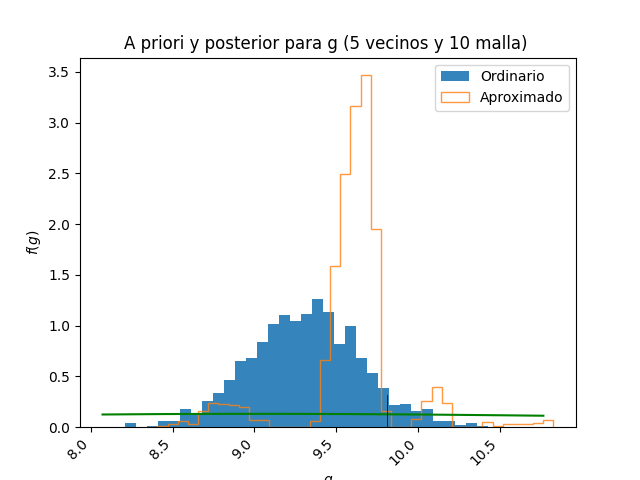
\includegraphics[width=0.4\textwidth]{img/Exp_Central_gravedad_sigma/Figuras/Individual/PostAprox_theta1_1_gravedad_sigma.png}
% %     \label{fig:subfig1}}
% %     \qquad
% %     \subfloat[Subfigure 2 list of figures text][Posterior con Forward aproximado en malla de 15x15]{
% %     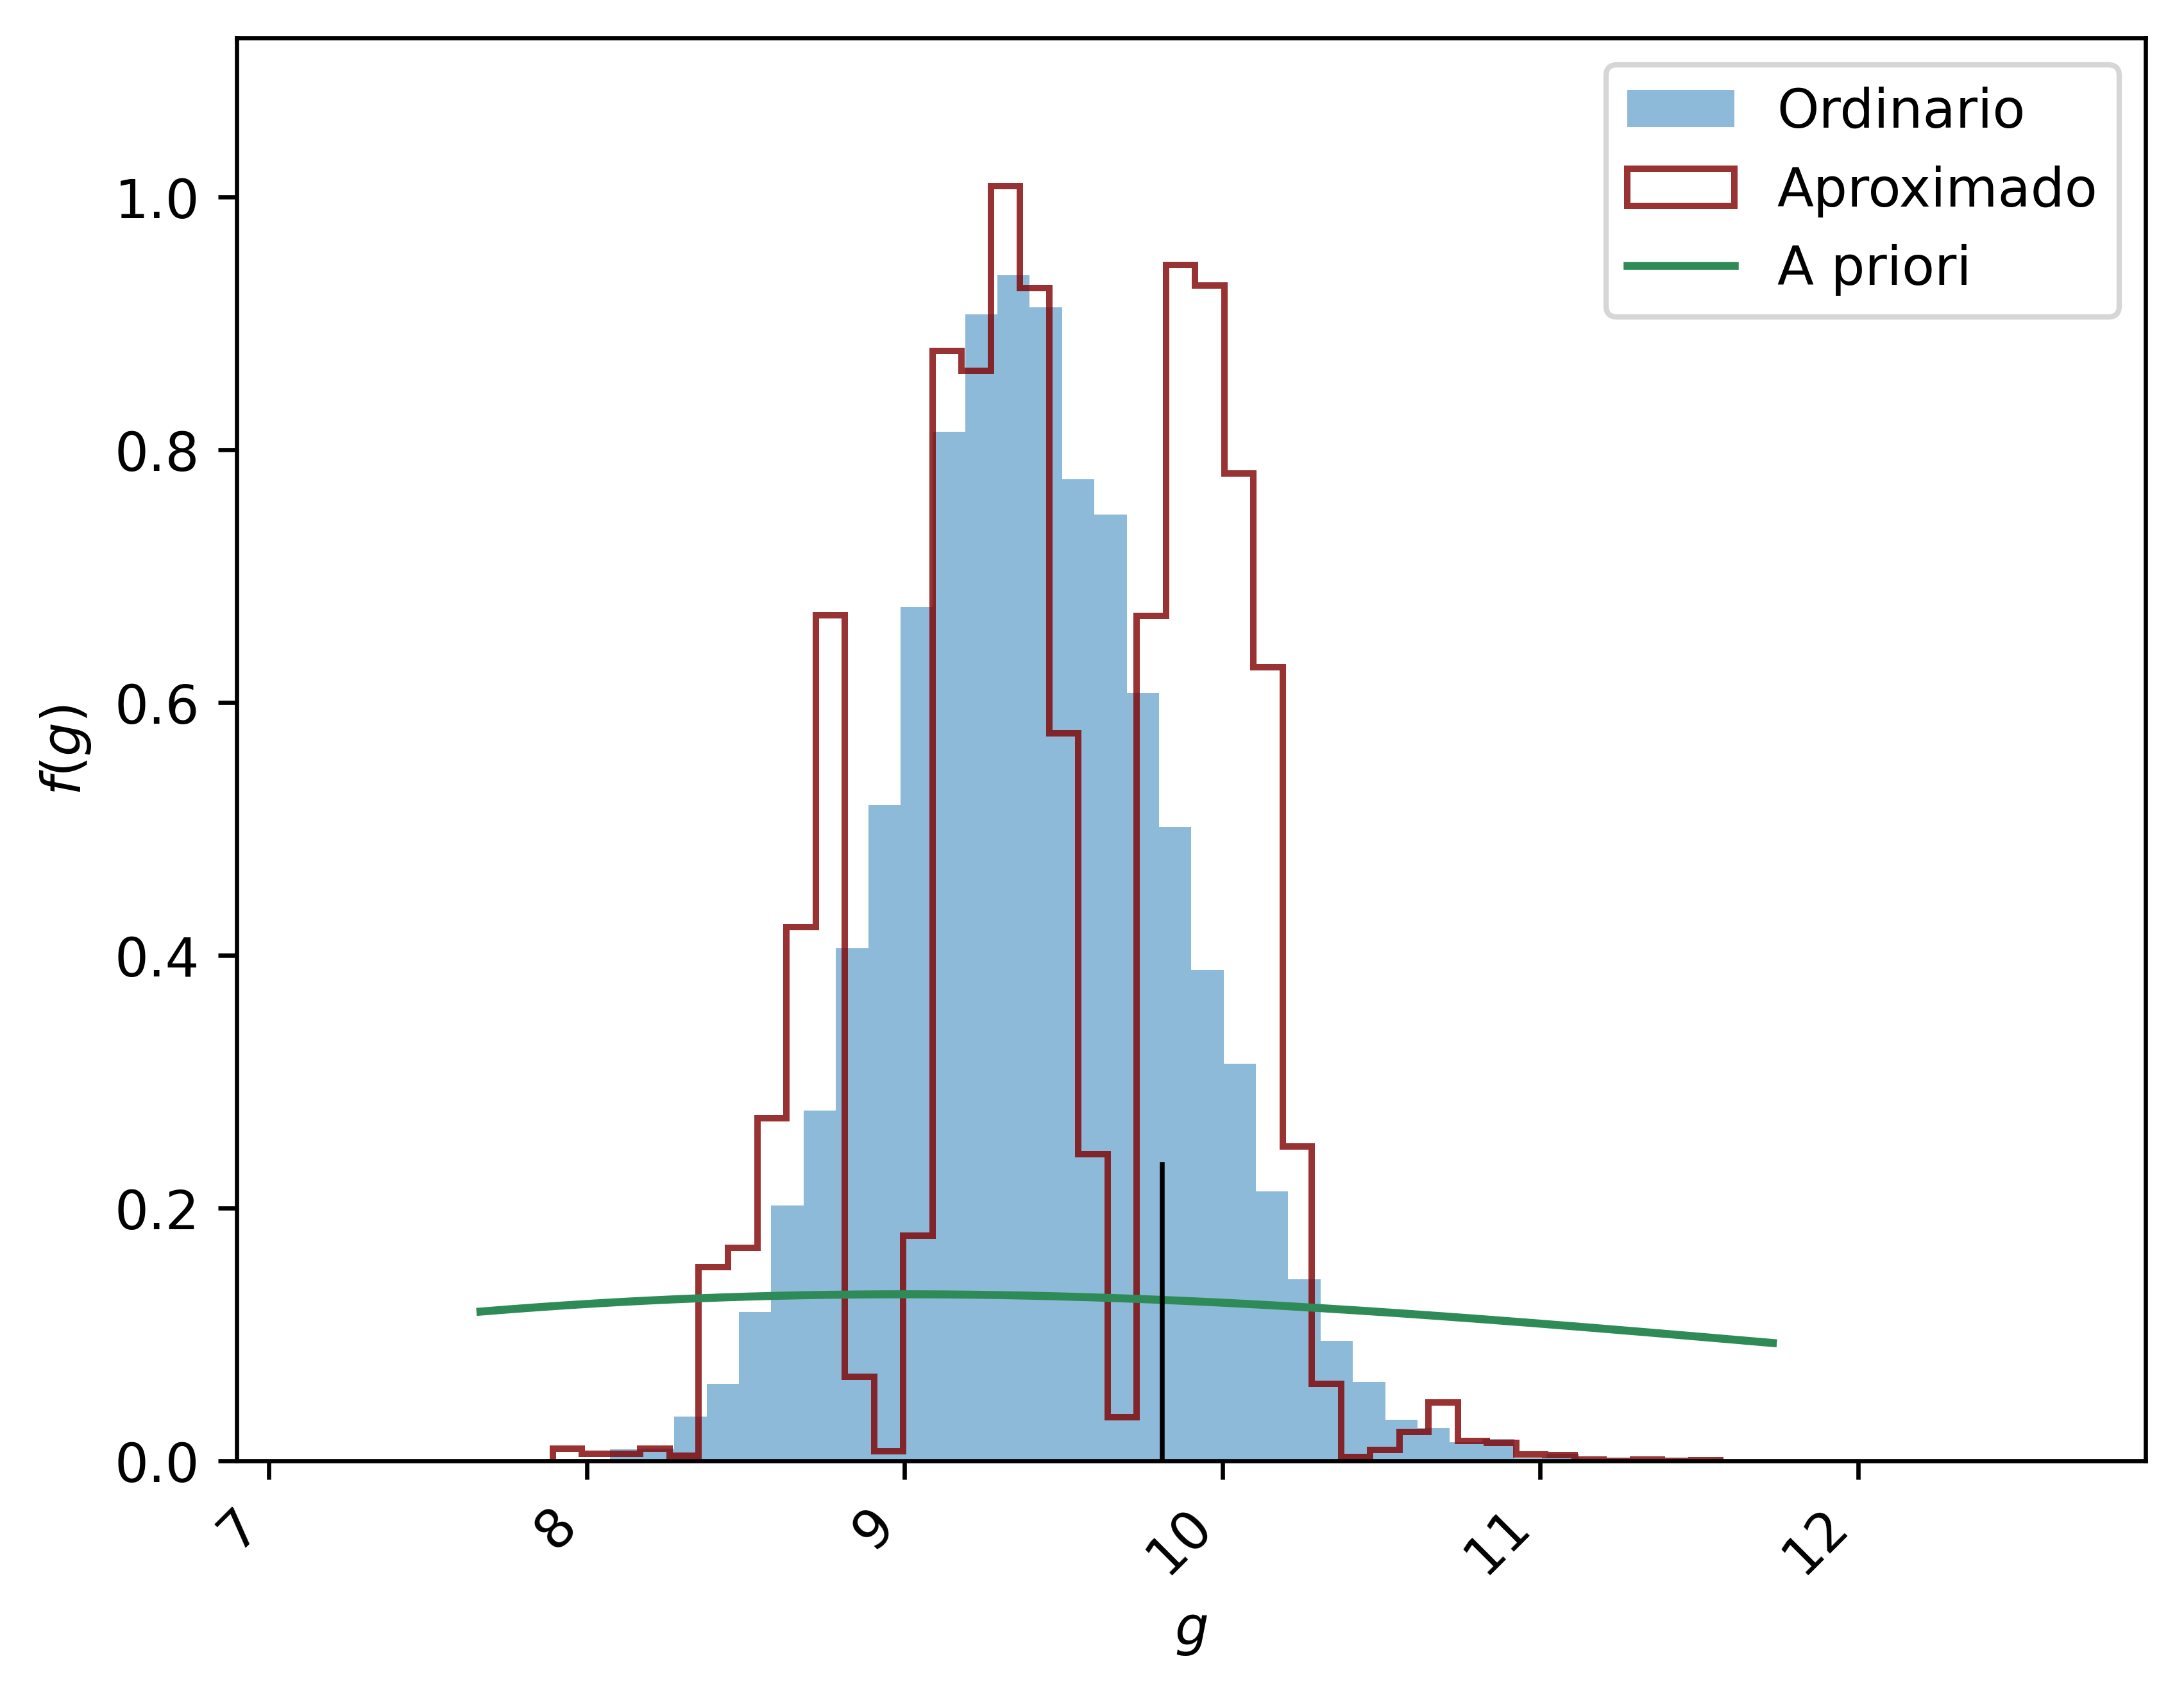
\includegraphics[width=0.4\textwidth]{img/Exp_Central_gravedad_sigma/Figuras/Individual/PostAprox_theta1_2_gravedad_sigma.png}
% %     \label{fig:subfig2}}
% %     \\
% %     \subfloat[Subfigure 3 list of figures text][Posterior con Forward aproximado en malla de 30x30]{
% %     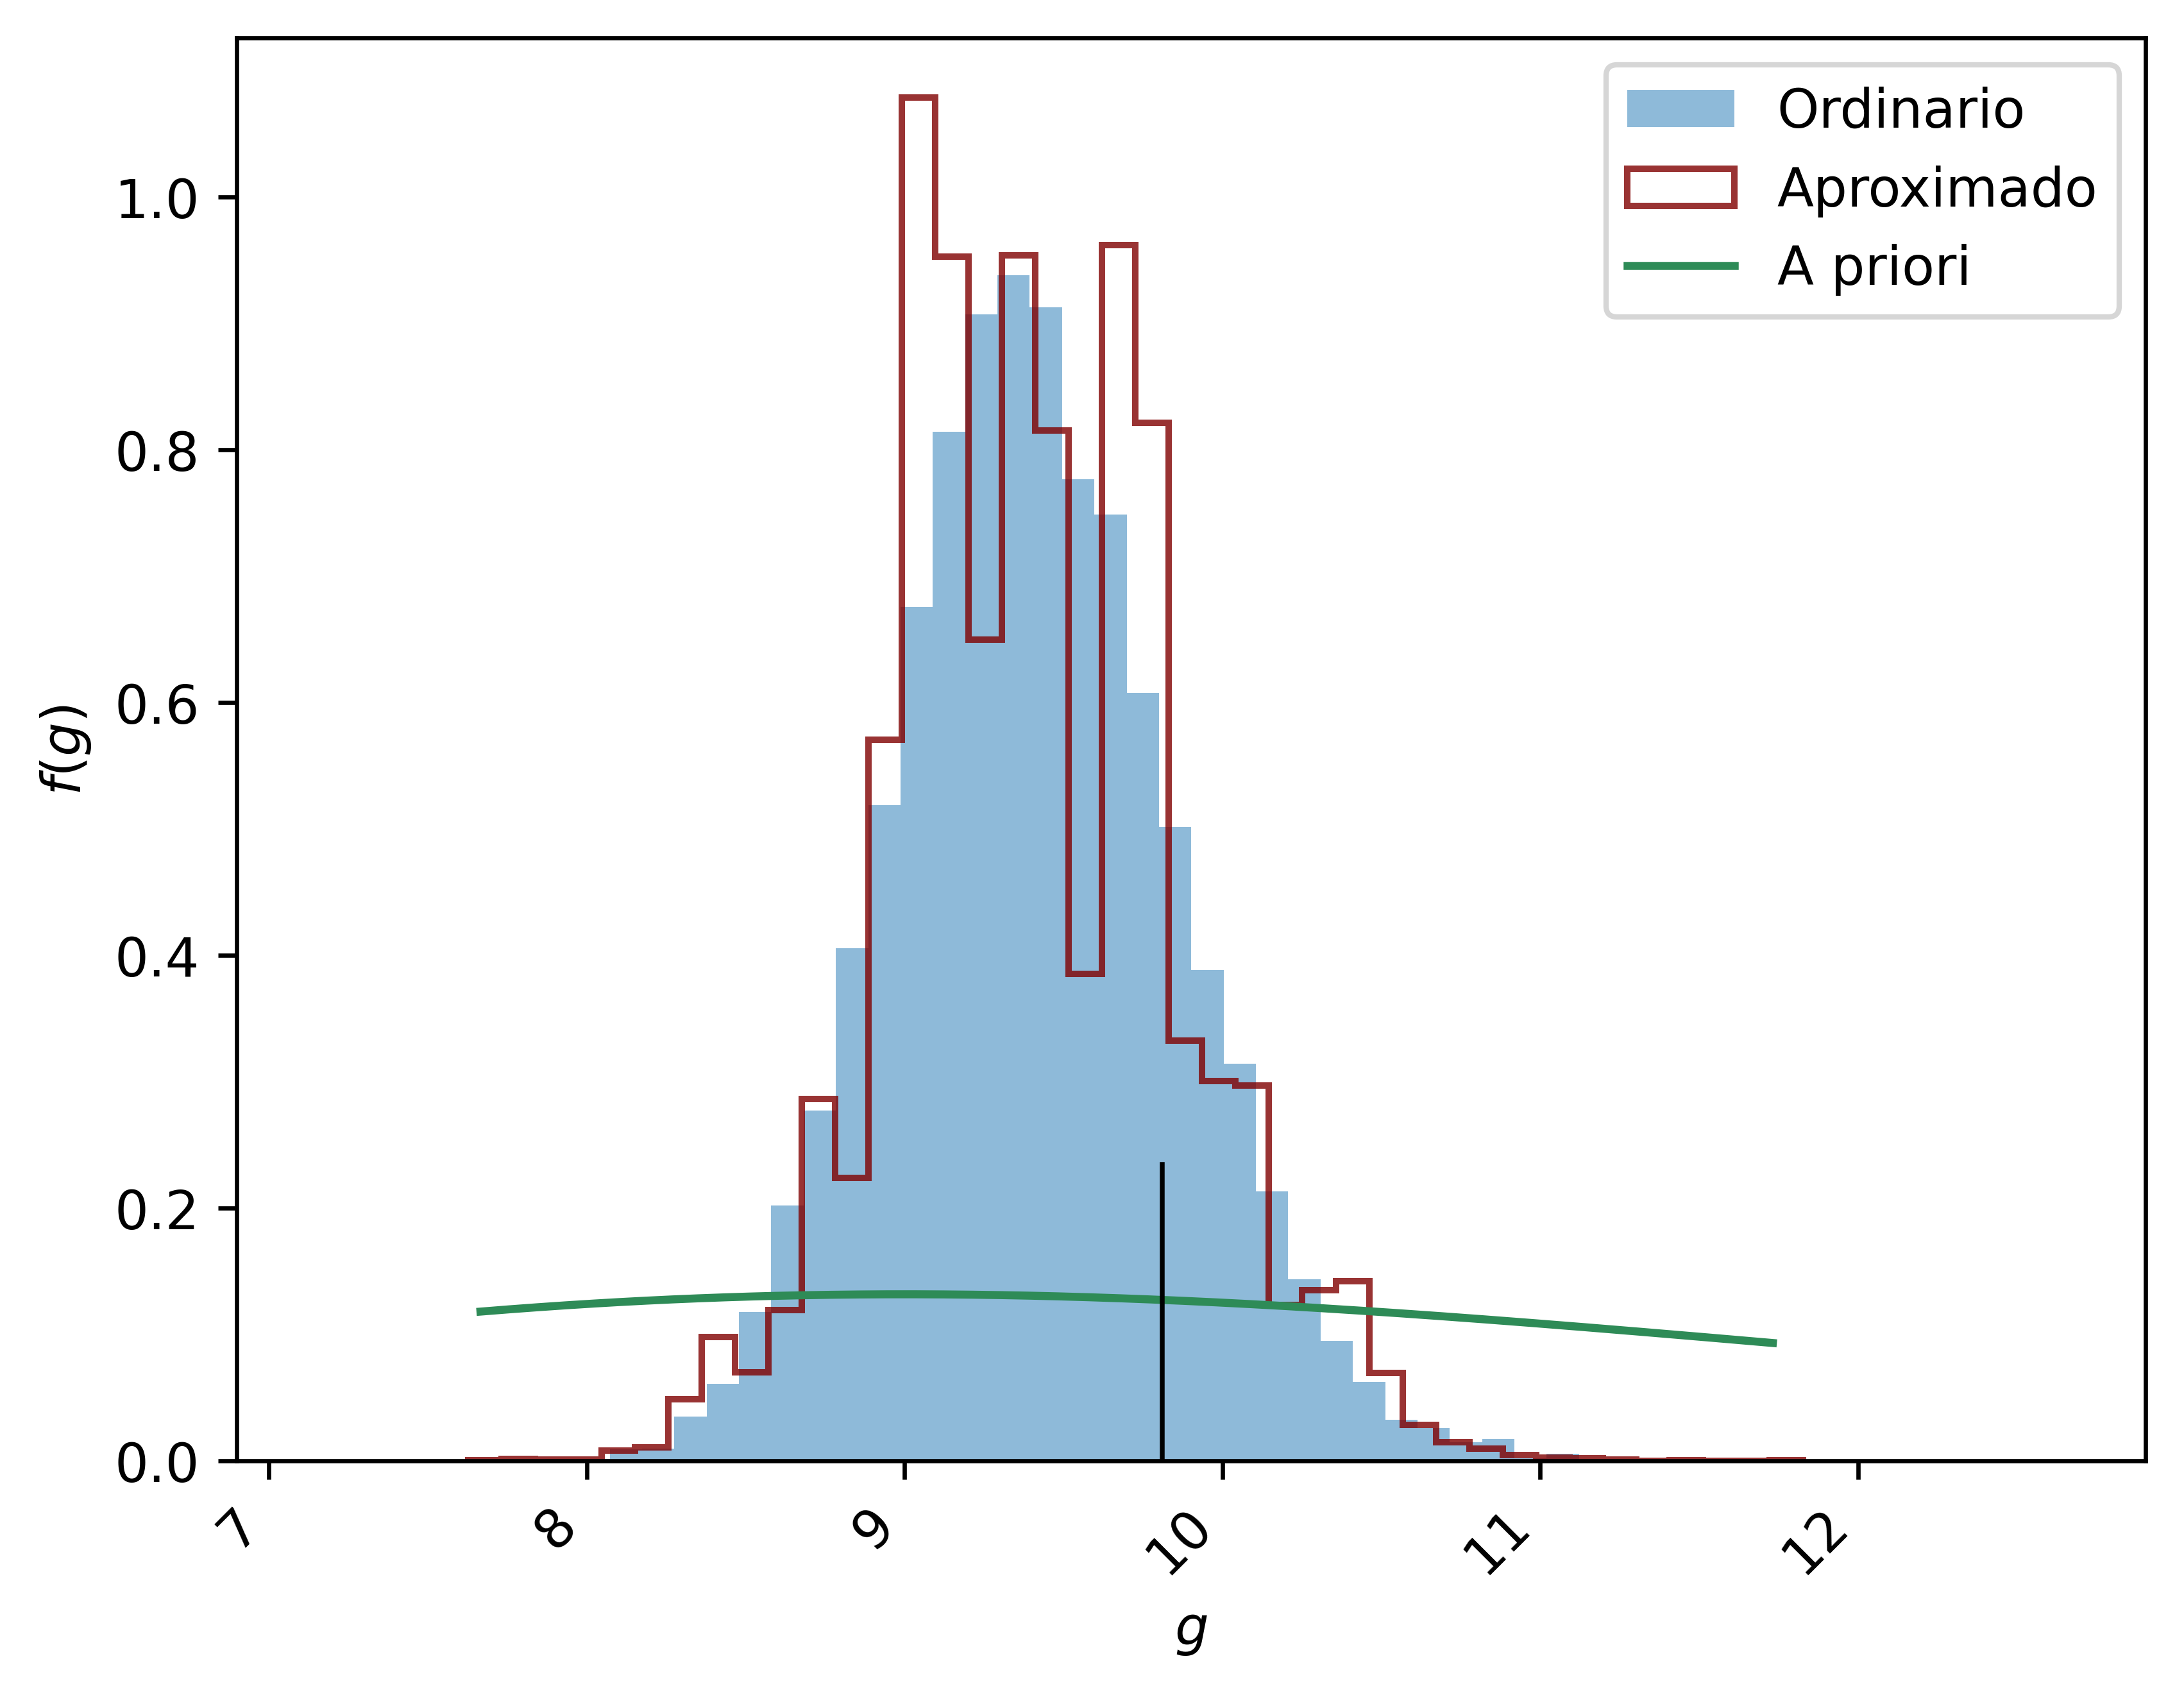
\includegraphics[width=0.4\textwidth]{img/Exp_Central_gravedad_sigma/Figuras/Individual/PostAprox_theta1_3_gravedad_sigma.png}
% %     \label{fig:subfig3}}
% %     \qquad
% %     \subfloat[Subfigure 4 list of figures text][Posterior con Forward aproximado en malla de 50x50]{
% %     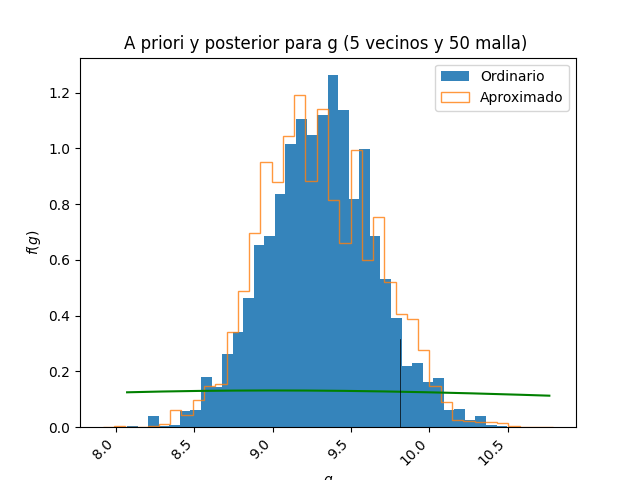
\includegraphics[width=0.4\textwidth]{img/Exp_Central_gravedad_sigma/Figuras/Individual/PostAprox_theta1_4_gravedad_sigma.png}
% %     \label{fig:subfig4}}
% %     \caption{Distribución posterior para $g$ con Forward ordinario y Forward aproximado con 5 vecinos cercanos.}
% %     \label{fig:g_01}
% % \end{figure}


% % \begin{figure}[h]
% %     \centering
% %     \subfloat[Subfigure 1 list of figures text][Posterior con Forward aproximado en malla de 10x10]{
% %     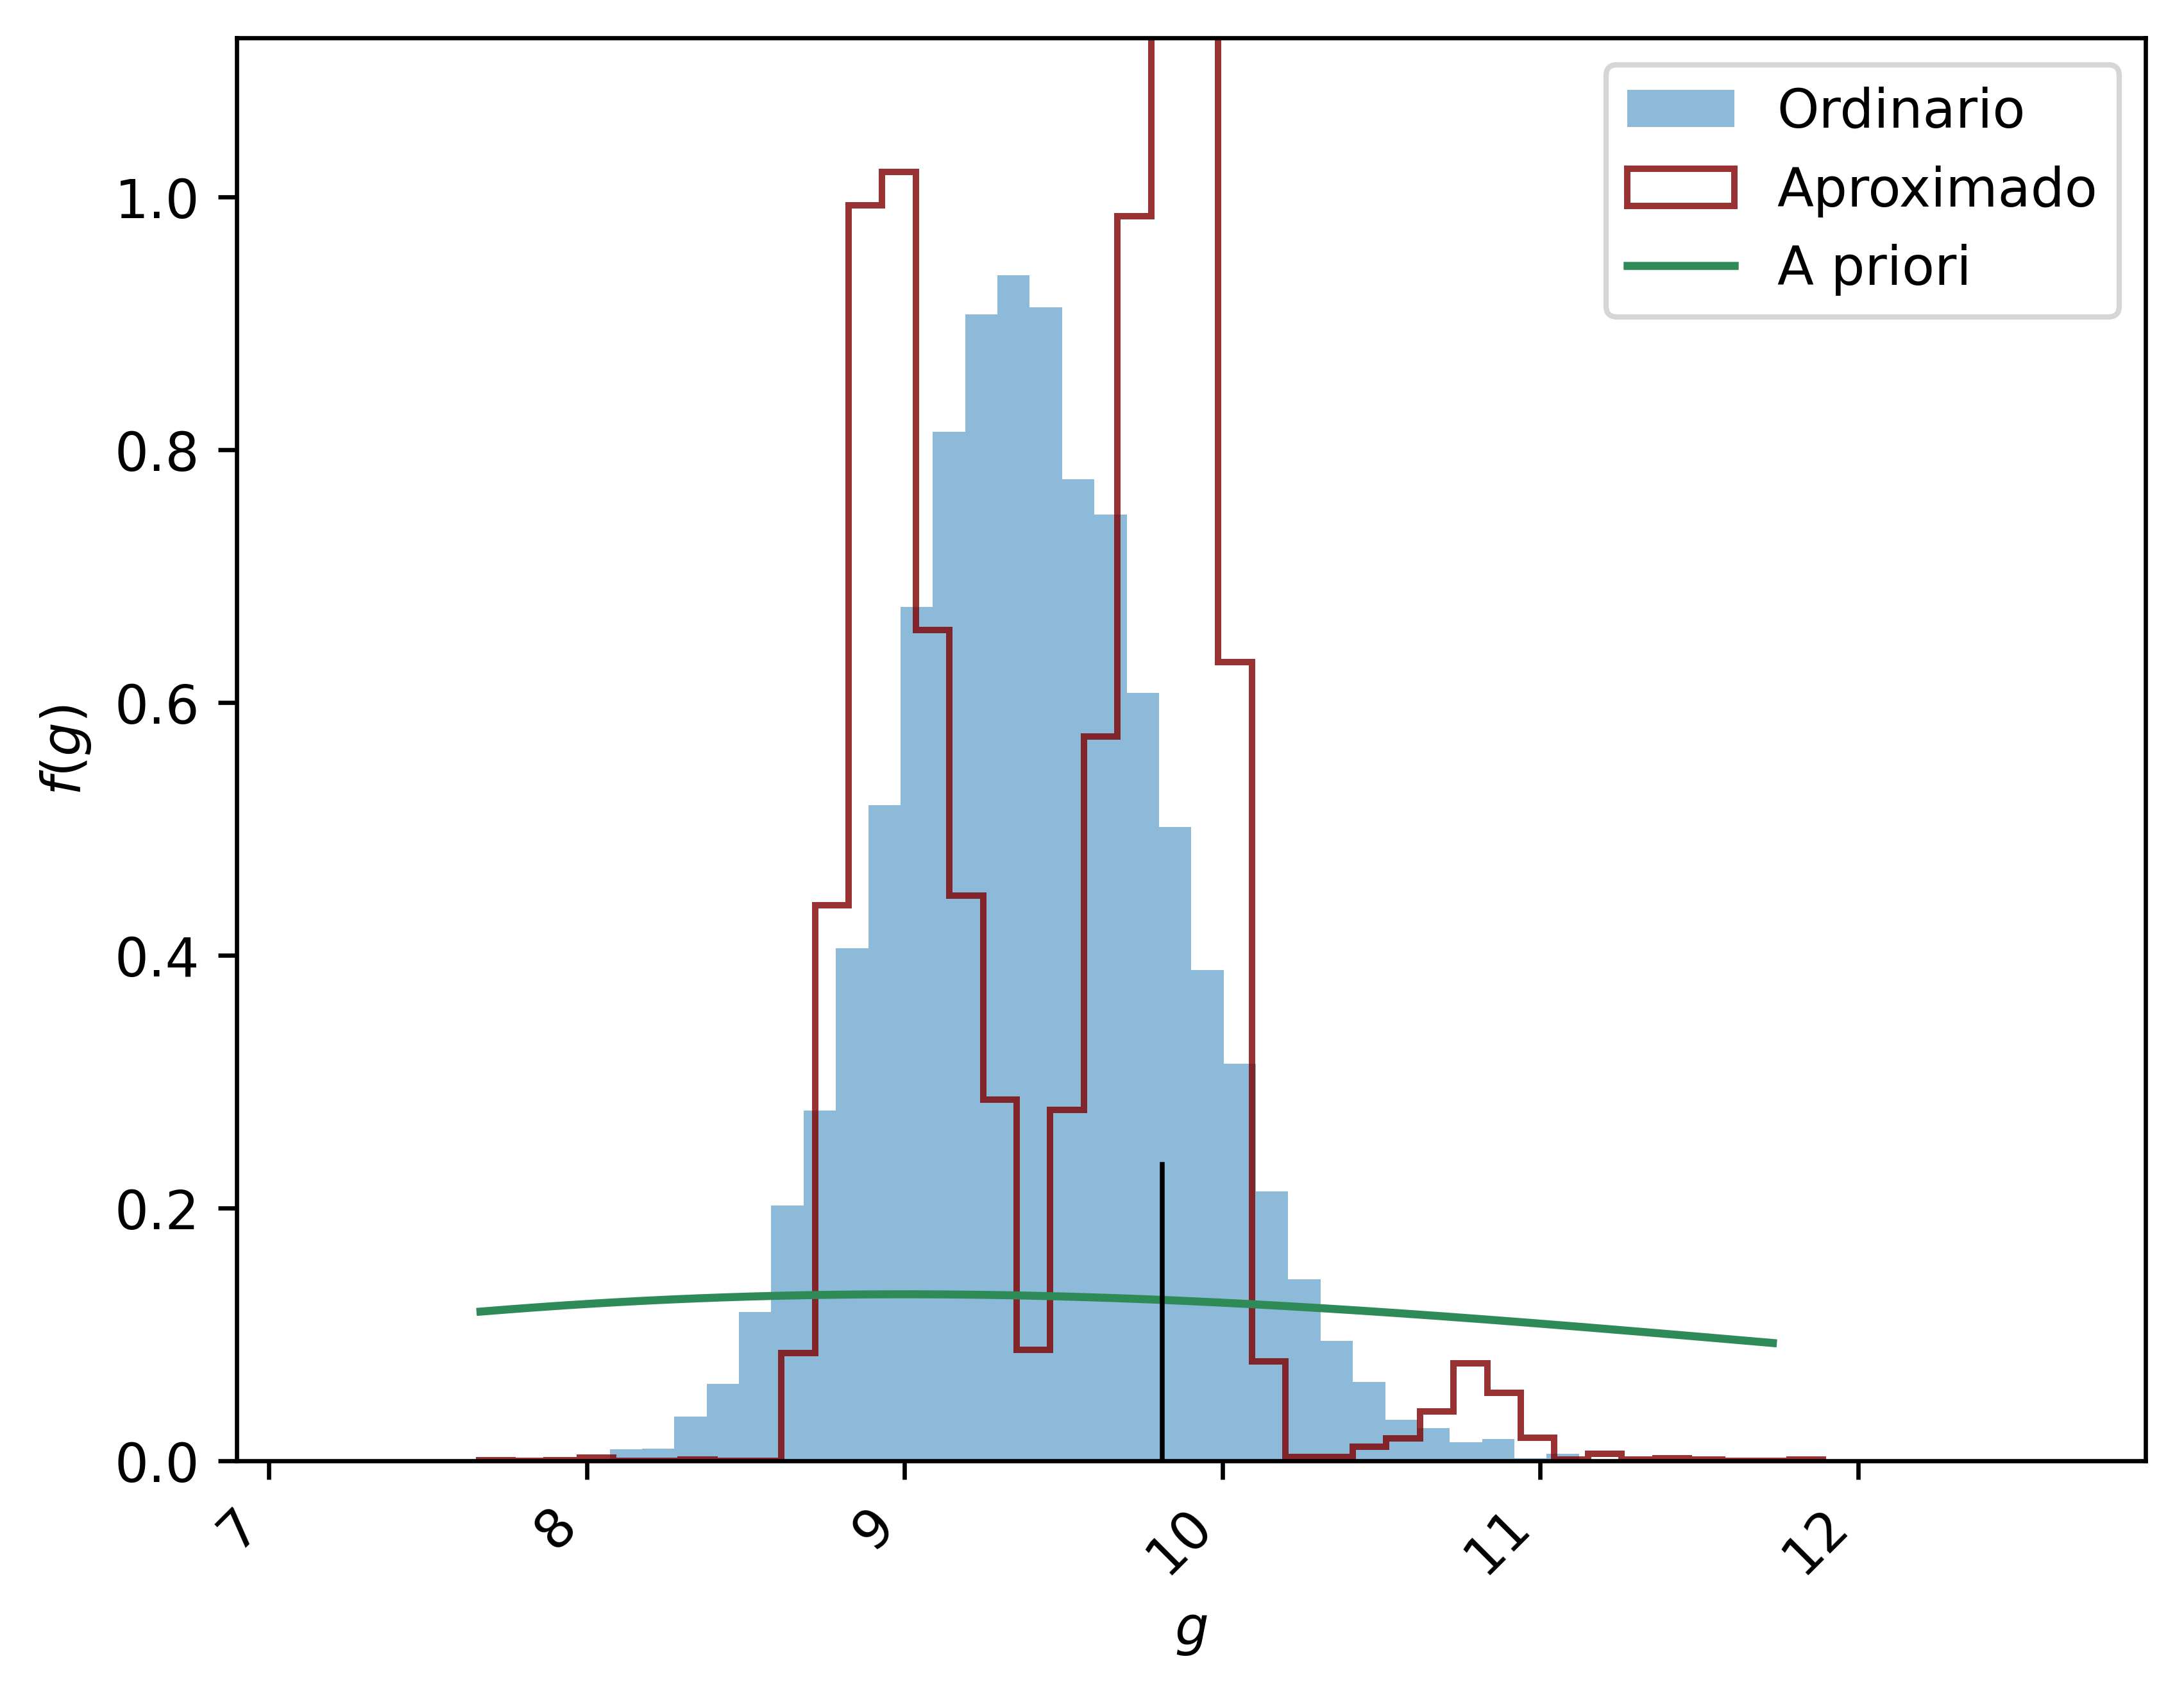
\includegraphics[width=0.4\textwidth]{img/Exp_Central_gravedad_sigma/Figuras/Individual/PostAprox_theta1_5_gravedad_sigma.png}
% %     \label{fig:subfig1}}
% %     \qquad
% %     \subfloat[Subfigure 2 list of figures text][Posterior con Forward aproximado en malla de 15x15]{
% %     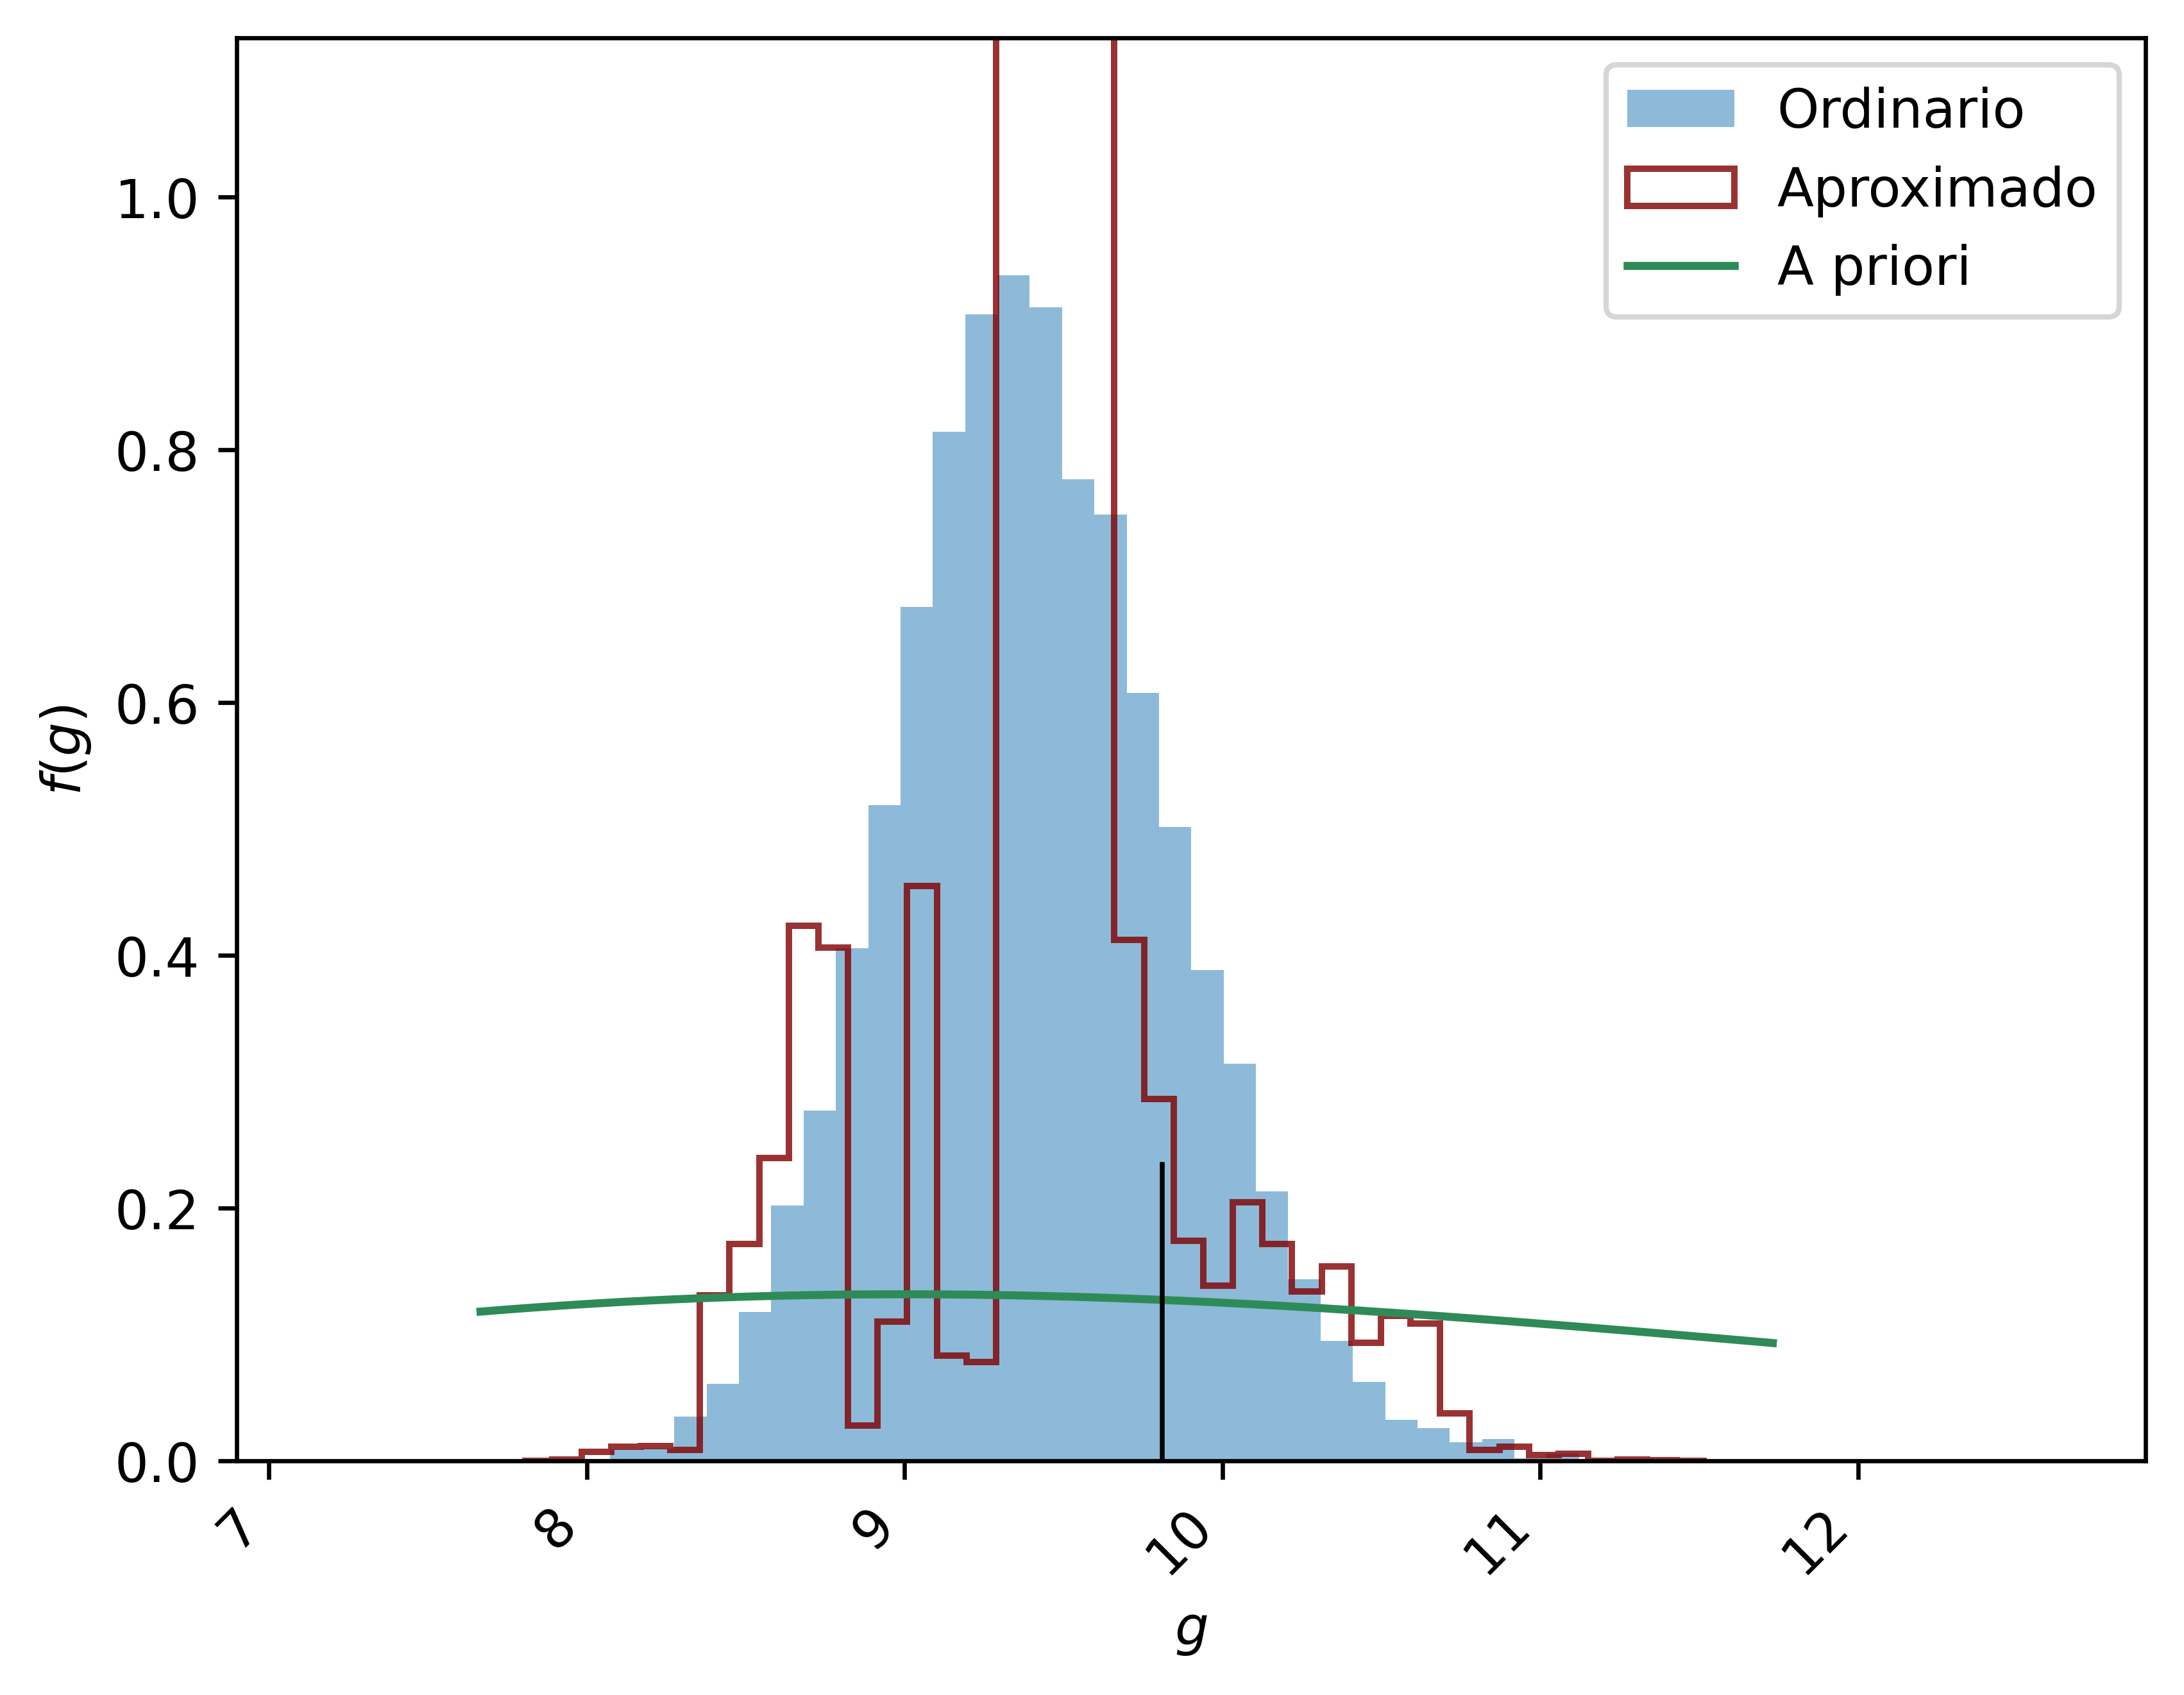
\includegraphics[width=0.4\textwidth]{img/Exp_Central_gravedad_sigma/Figuras/Individual/PostAprox_theta1_6_gravedad_sigma.png}
% %     \label{fig:subfig2}}
% %     \\
% %     \subfloat[Subfigure 3 list of figures text][Posterior con Forward aproximado en malla de 30x30]{
% %     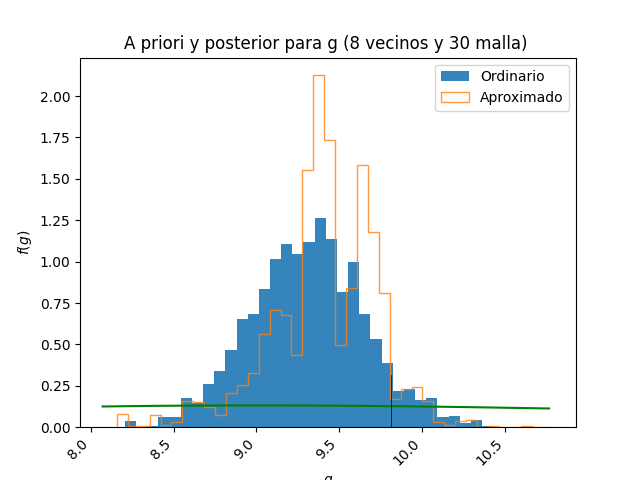
\includegraphics[width=0.4\textwidth]{img/Exp_Central_gravedad_sigma/Figuras/Individual/PostAprox_theta1_7_gravedad_sigma.png}
% %     \label{fig:subfig3}}
% %     \qquad
% %     \subfloat[Subfigure 4 list of figures text][Posterior con Forward aproximado en malla de 50x50]{
% %     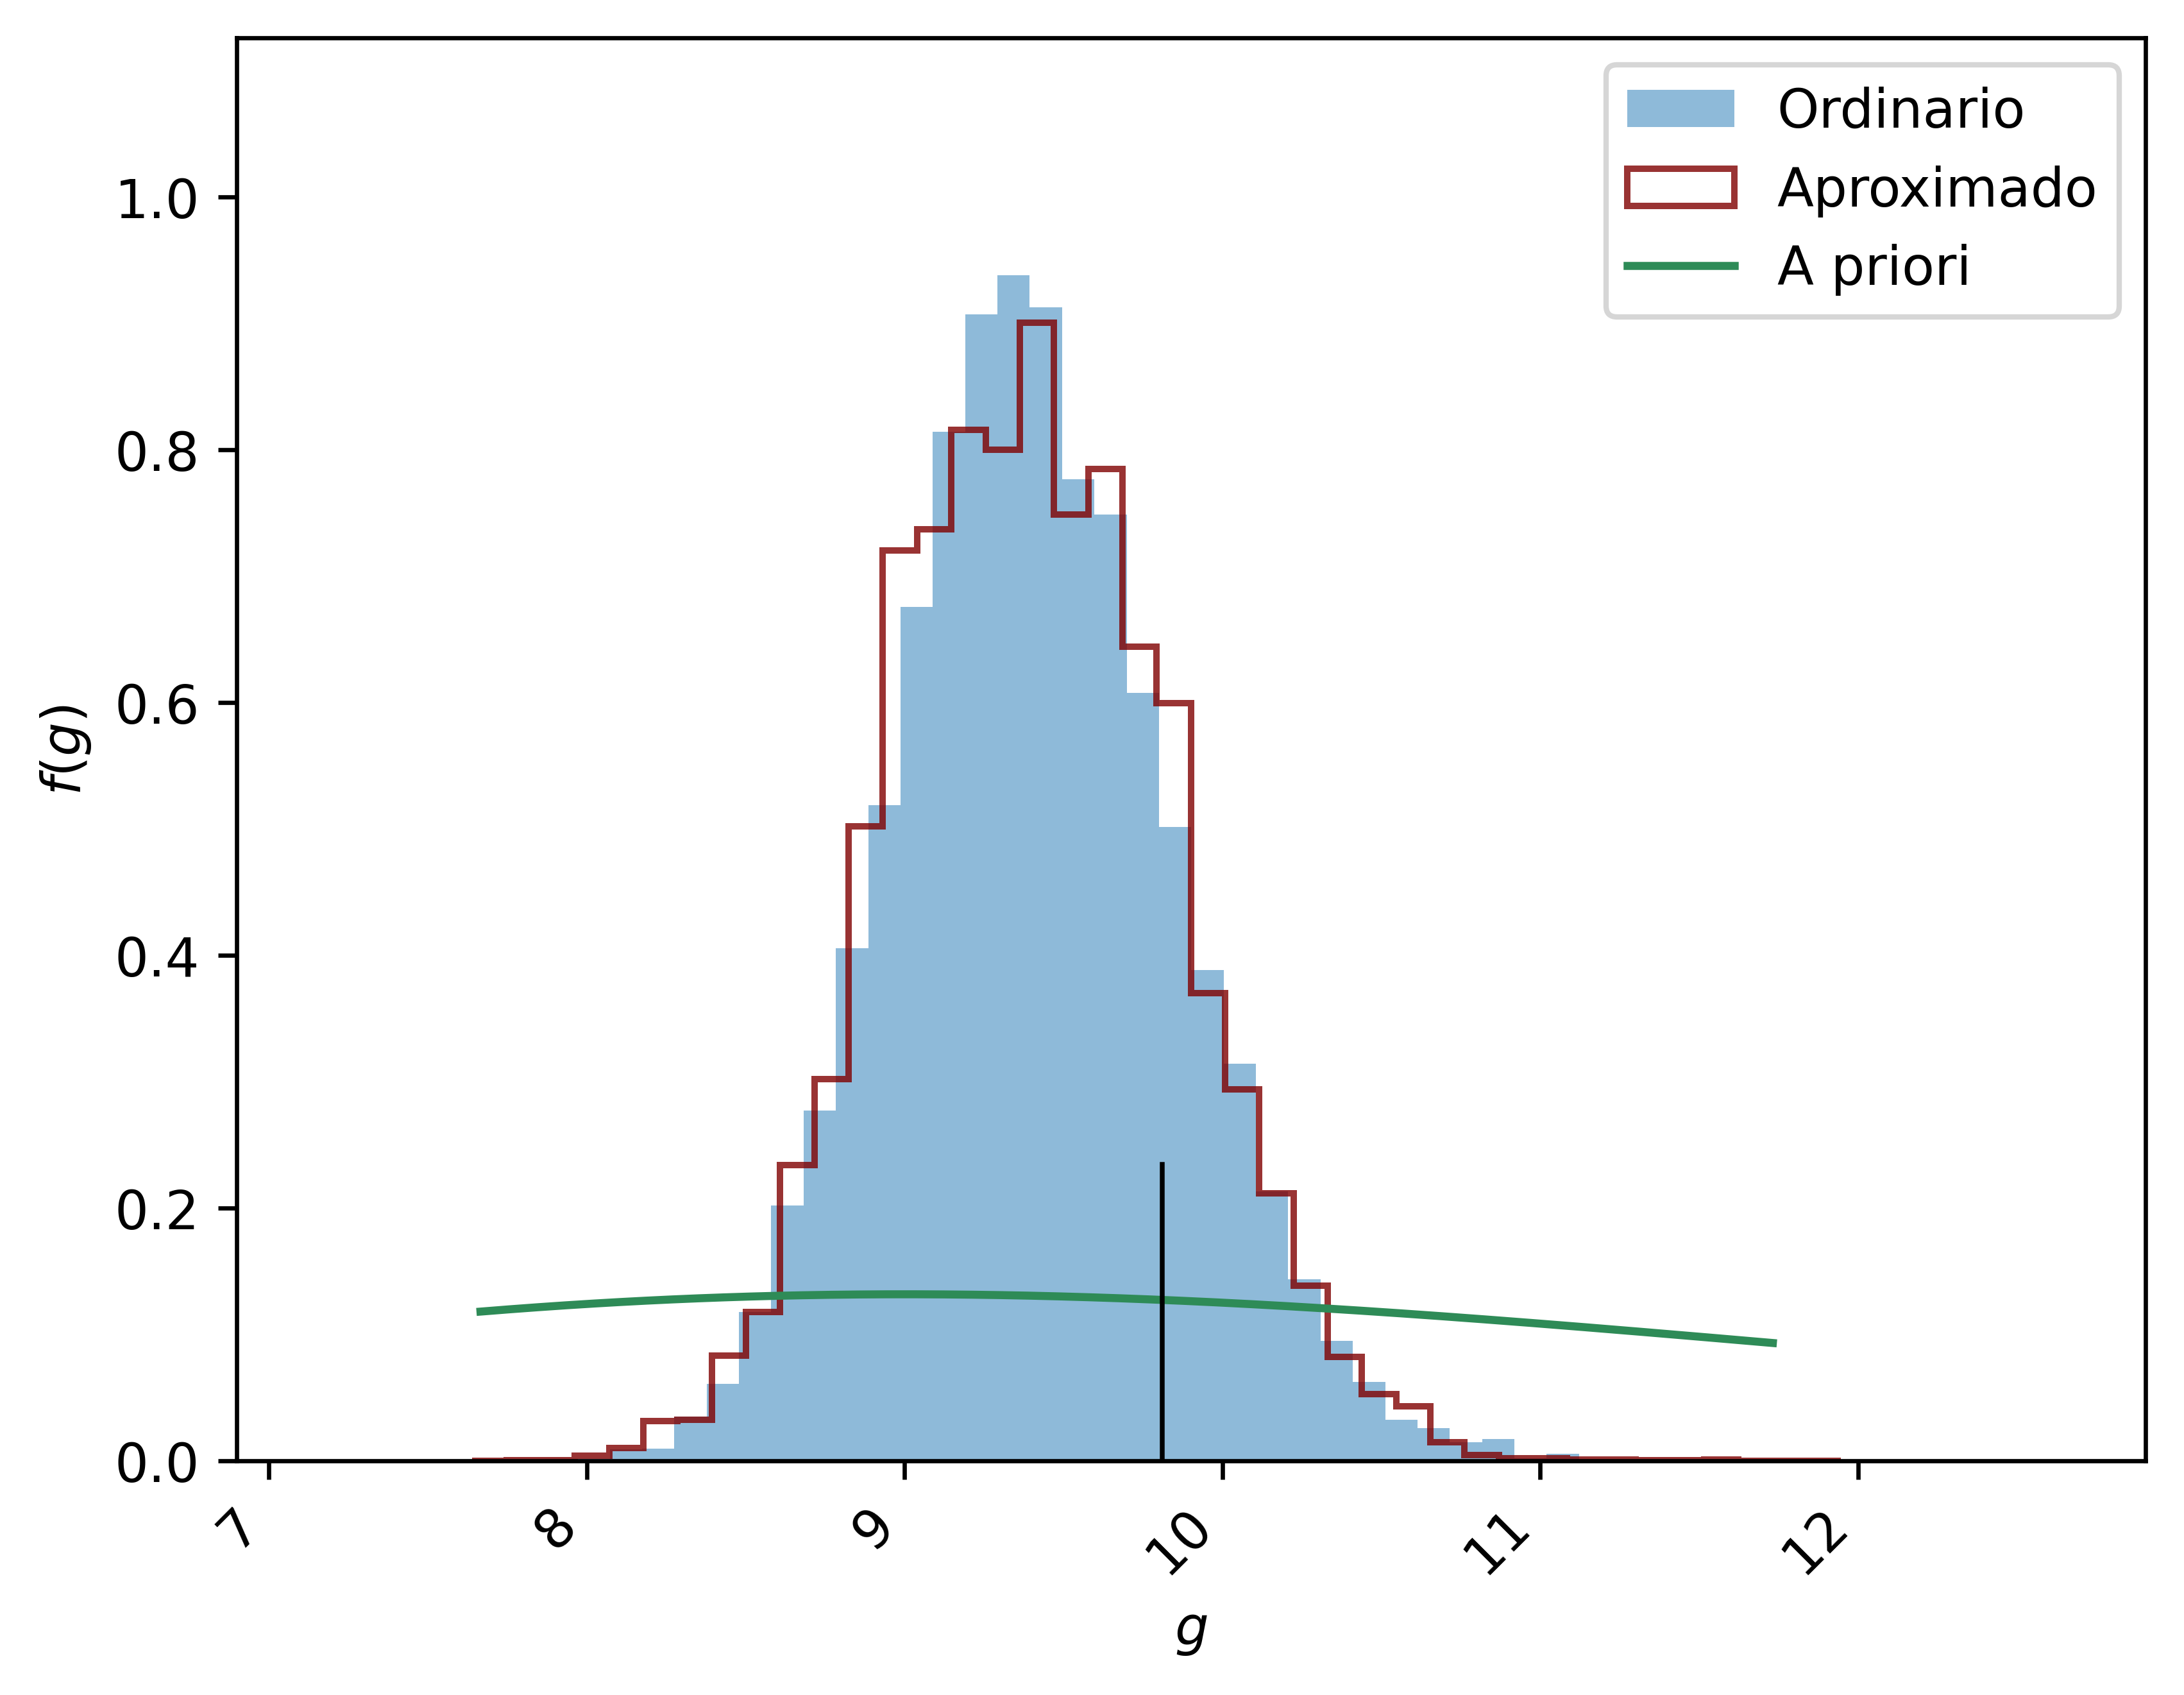
\includegraphics[width=0.4\textwidth]{img/Exp_Central_gravedad_sigma/Figuras/Individual/PostAprox_theta1_8_gravedad_sigma.png}
% %     \label{fig:subfig4}}
% %     \caption{Distribución posterior para $g$ con Forward ordinario y Forward aproximado con 5 vecinos cercanos.}
% %     \label{fig:g_01}
% % \end{figure}


% % \begin{figure}[h]
% %     \centering
% %     \subfloat[Subfigure 1 list of figures text][Posterior con Forward aproximado en malla de 10x10]{
% %     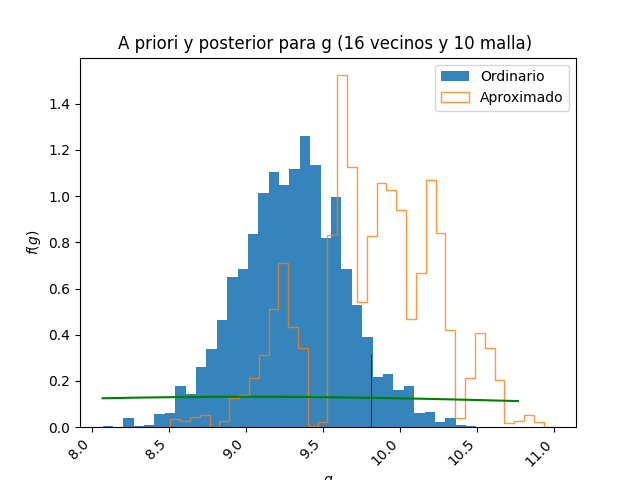
\includegraphics[width=0.4\textwidth]{img/Exp_Central_gravedad_sigma/Figuras/Individual/PostAprox_theta1_9_gravedad_sigma.png}
% %     \label{fig:subfig1}}
% %     \qquad
% %     \subfloat[Subfigure 2 list of figures text][Posterior con Forward aproximado en malla de 15x15]{
% %     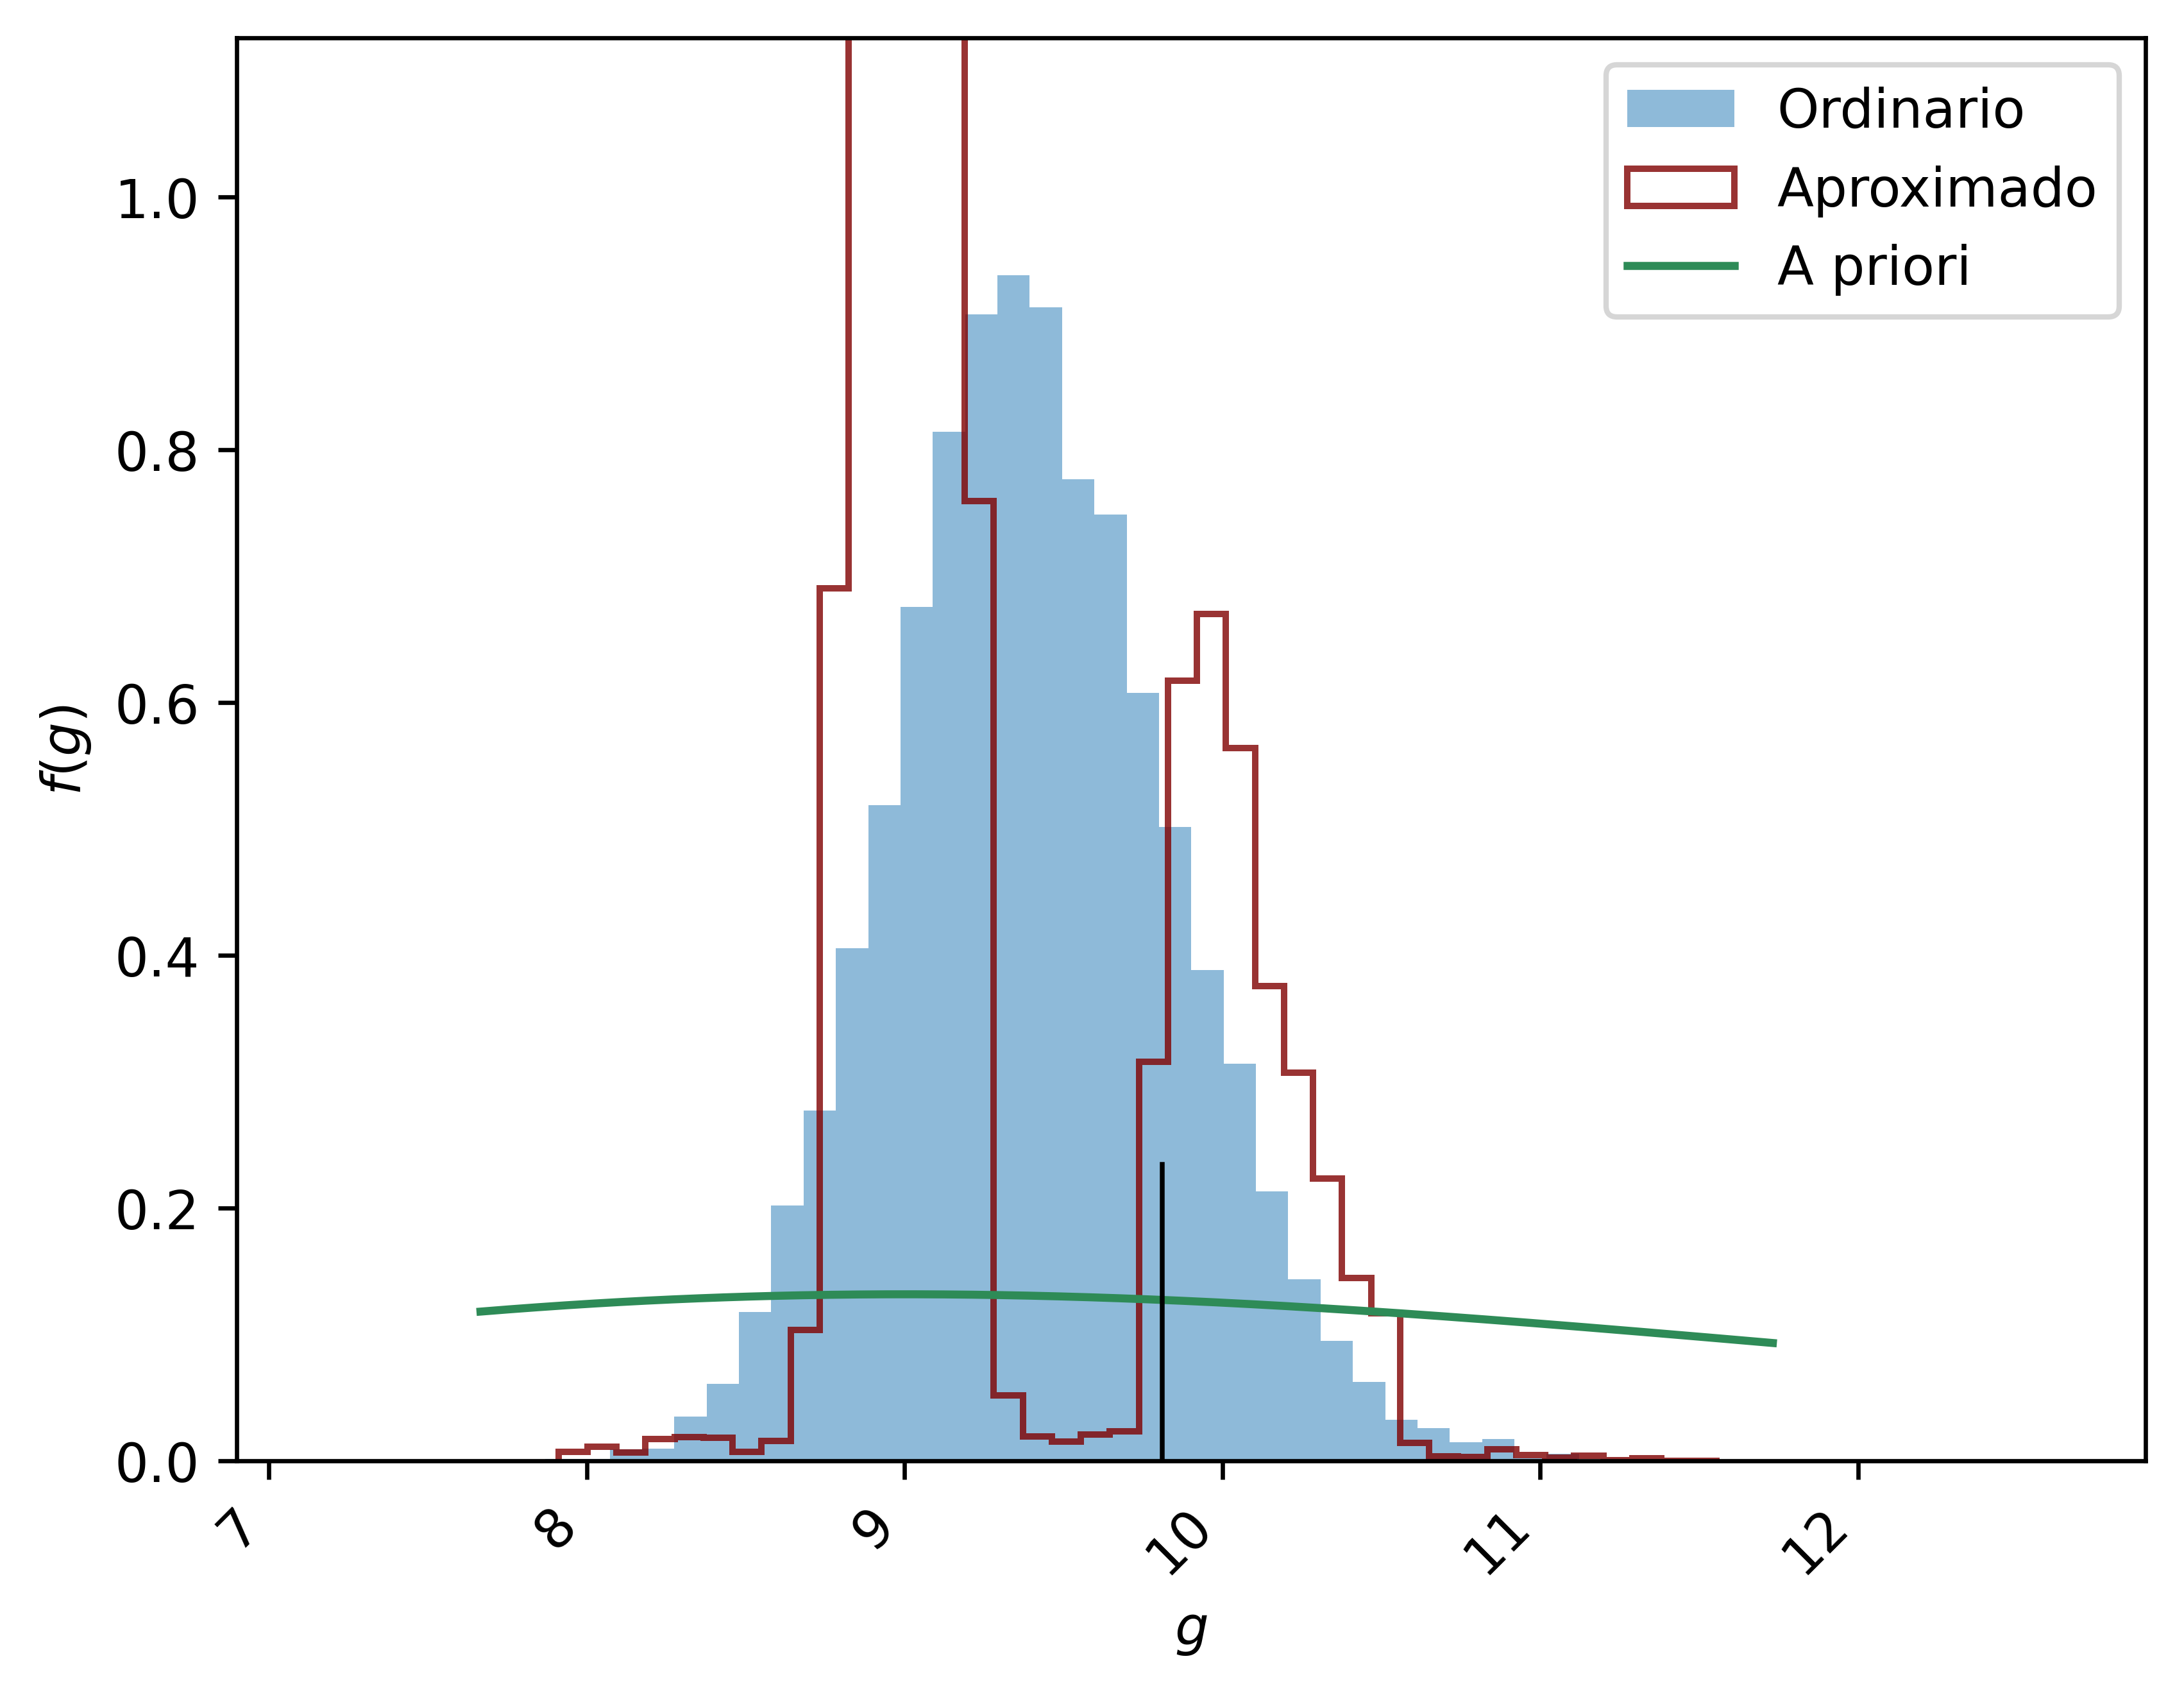
\includegraphics[width=0.4\textwidth]{img/Exp_Central_gravedad_sigma/Figuras/Individual/PostAprox_theta1_10_gravedad_sigma.png}
% %     \label{fig:subfig2}}
% %     \\
% %     \subfloat[Subfigure 3 list of figures text][Posterior con Forward aproximado en malla de 30x30]{
% %     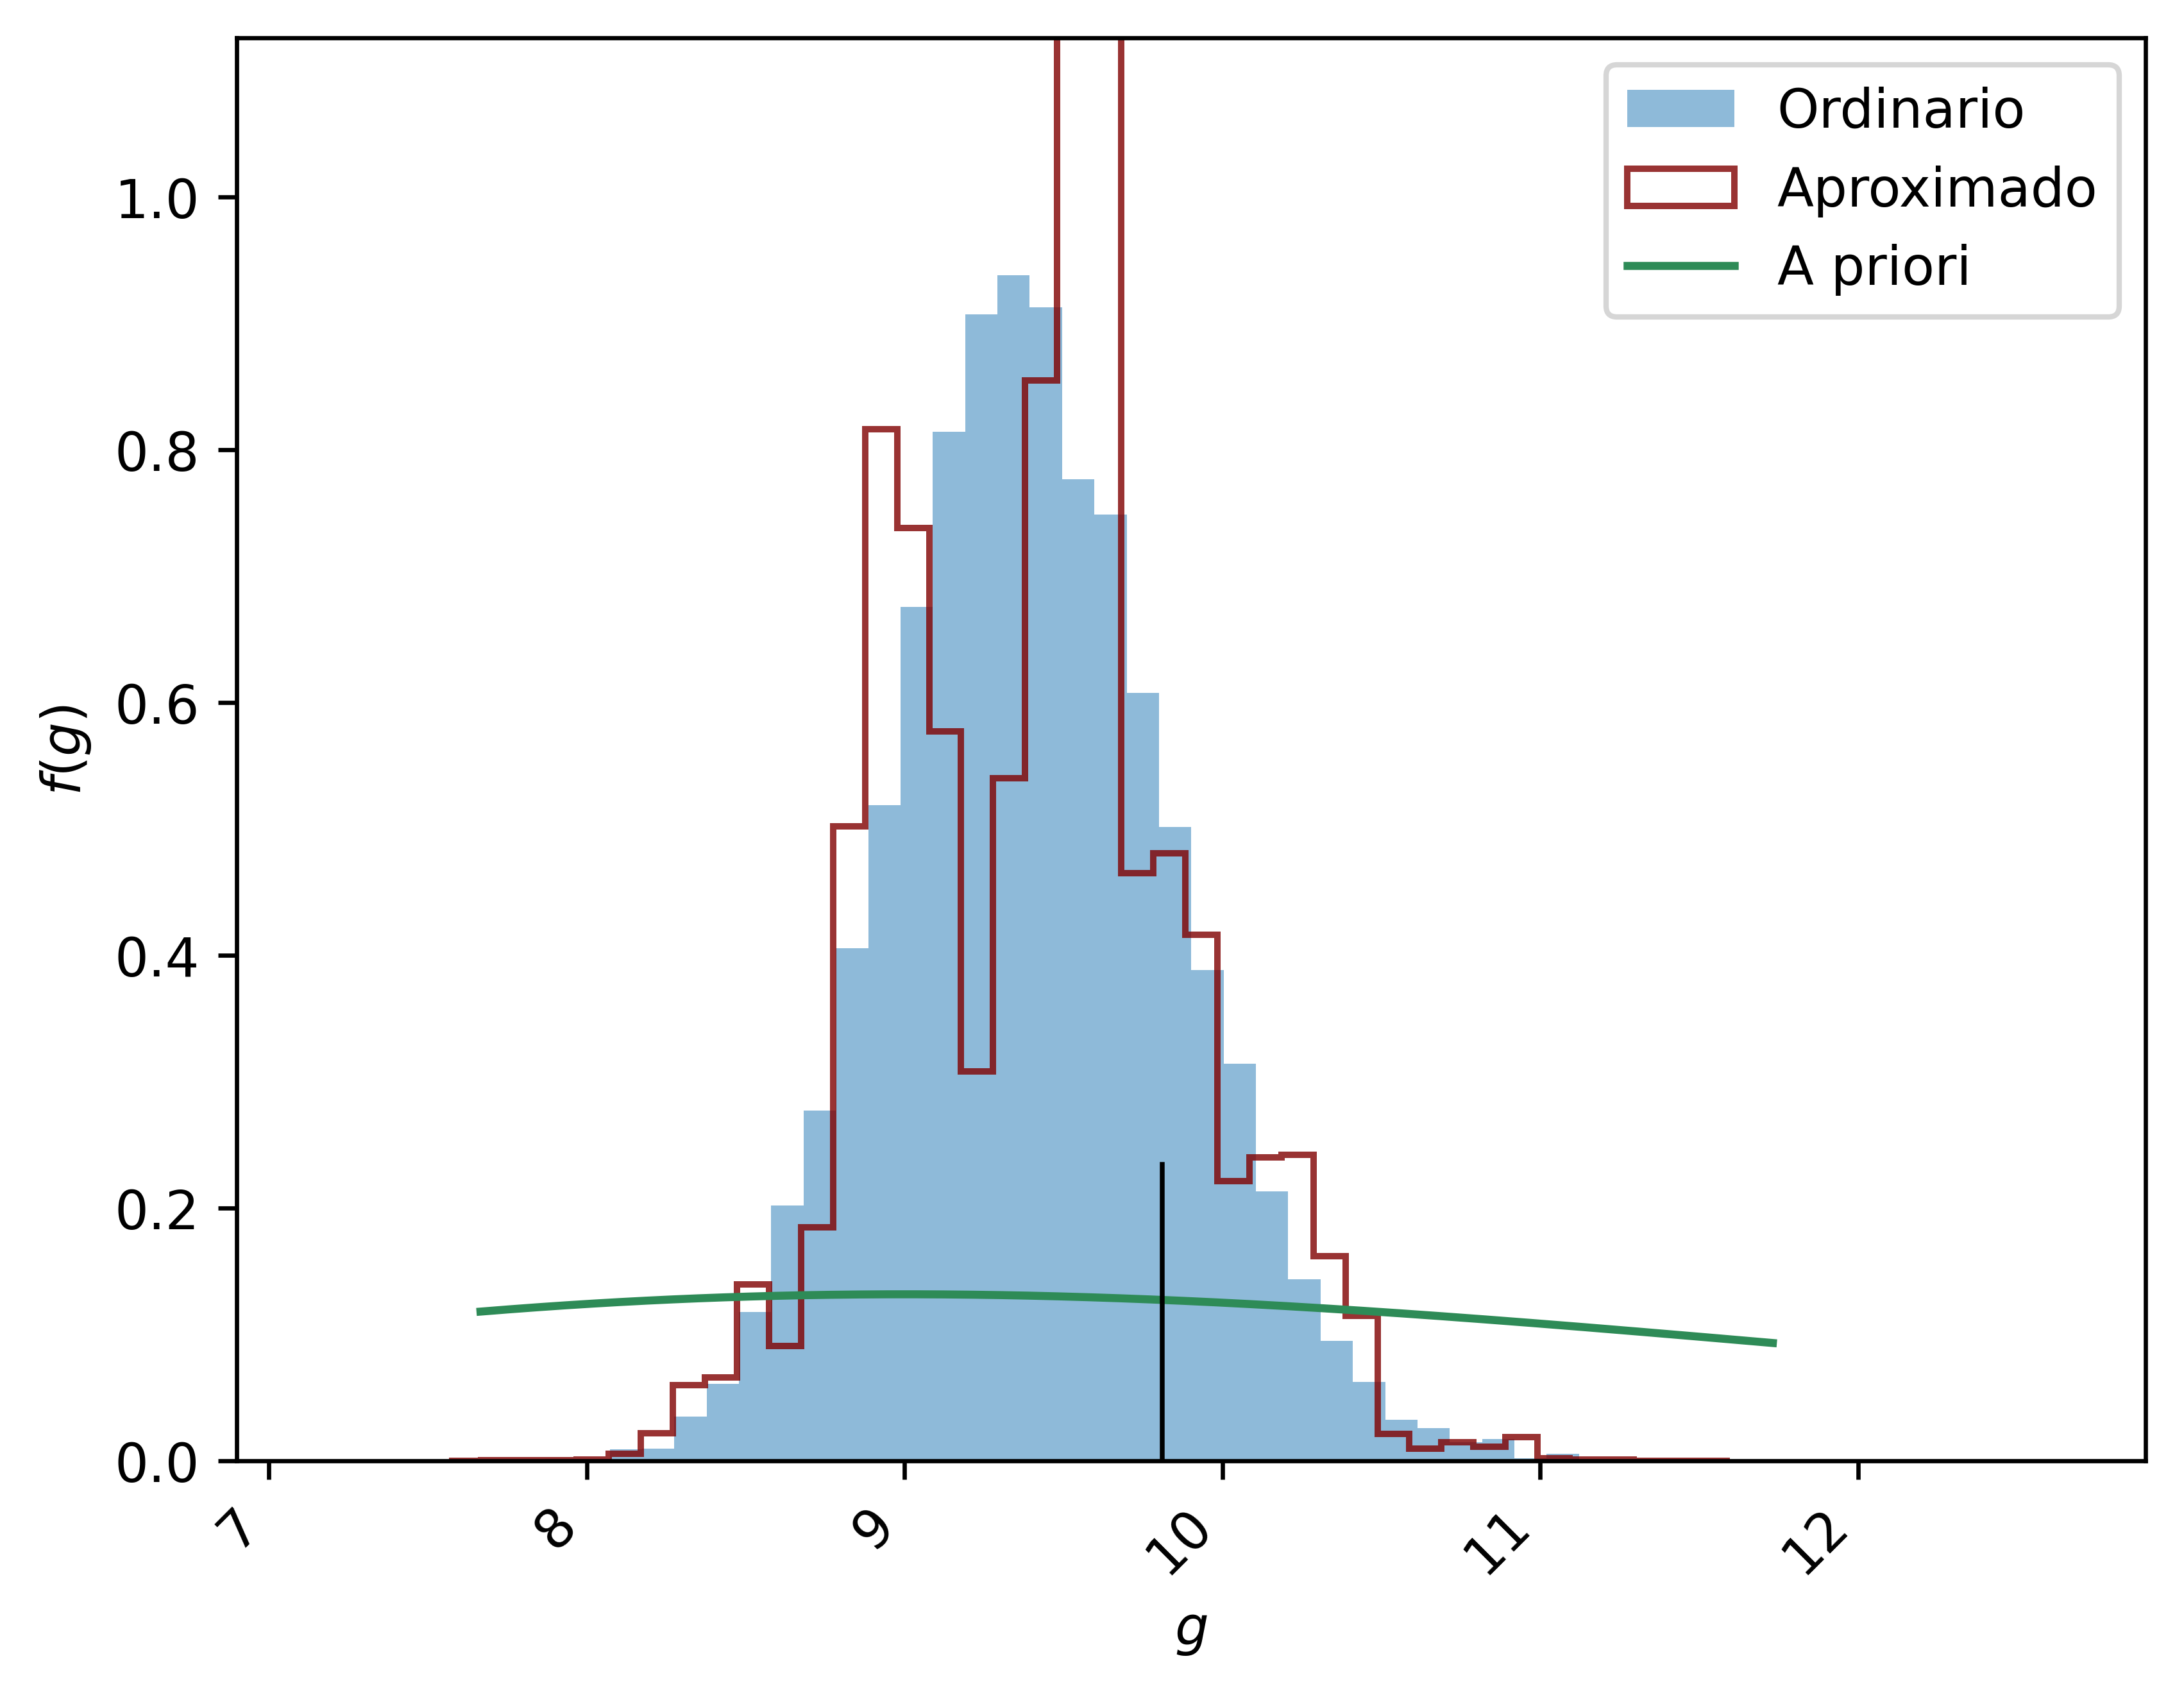
\includegraphics[width=0.4\textwidth]{img/Exp_Central_gravedad_sigma/Figuras/Individual/PostAprox_theta1_11_gravedad_sigma.png}
% %     \label{fig:subfig3}}
% %     \qquad
% %     \subfloat[Subfigure 4 list of figures text][Posterior con Forward aproximado en malla de 50x50]{
% %     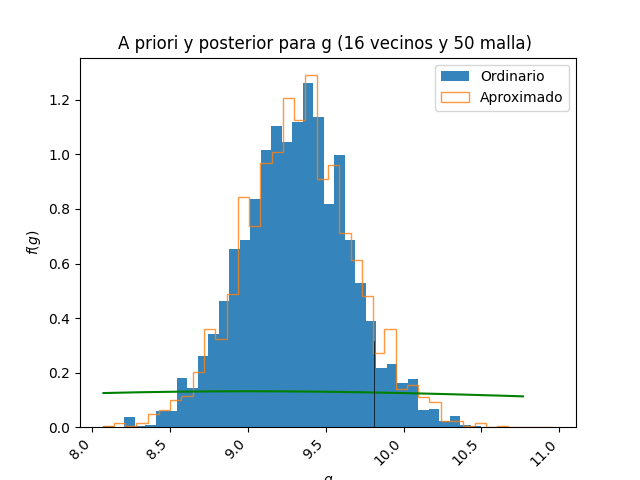
\includegraphics[width=0.4\textwidth]{img/Exp_Central_gravedad_sigma/Figuras/Individual/PostAprox_theta1_12_gravedad_sigma.png}
% %     \label{fig:subfig4}}
% %     \caption{Distribución posterior para $g$ con Forward ordinario y Forward aproximado con 5 vecinos cercanos.}
% %     \label{fig:g_01}
% % \end{figure}




% % \begin{figure}[h]
% %     \centering
% %     \subfloat[Subfigure 1 list of figures text][Posterior con Forward aproximado en malla de 10x10]{
% %     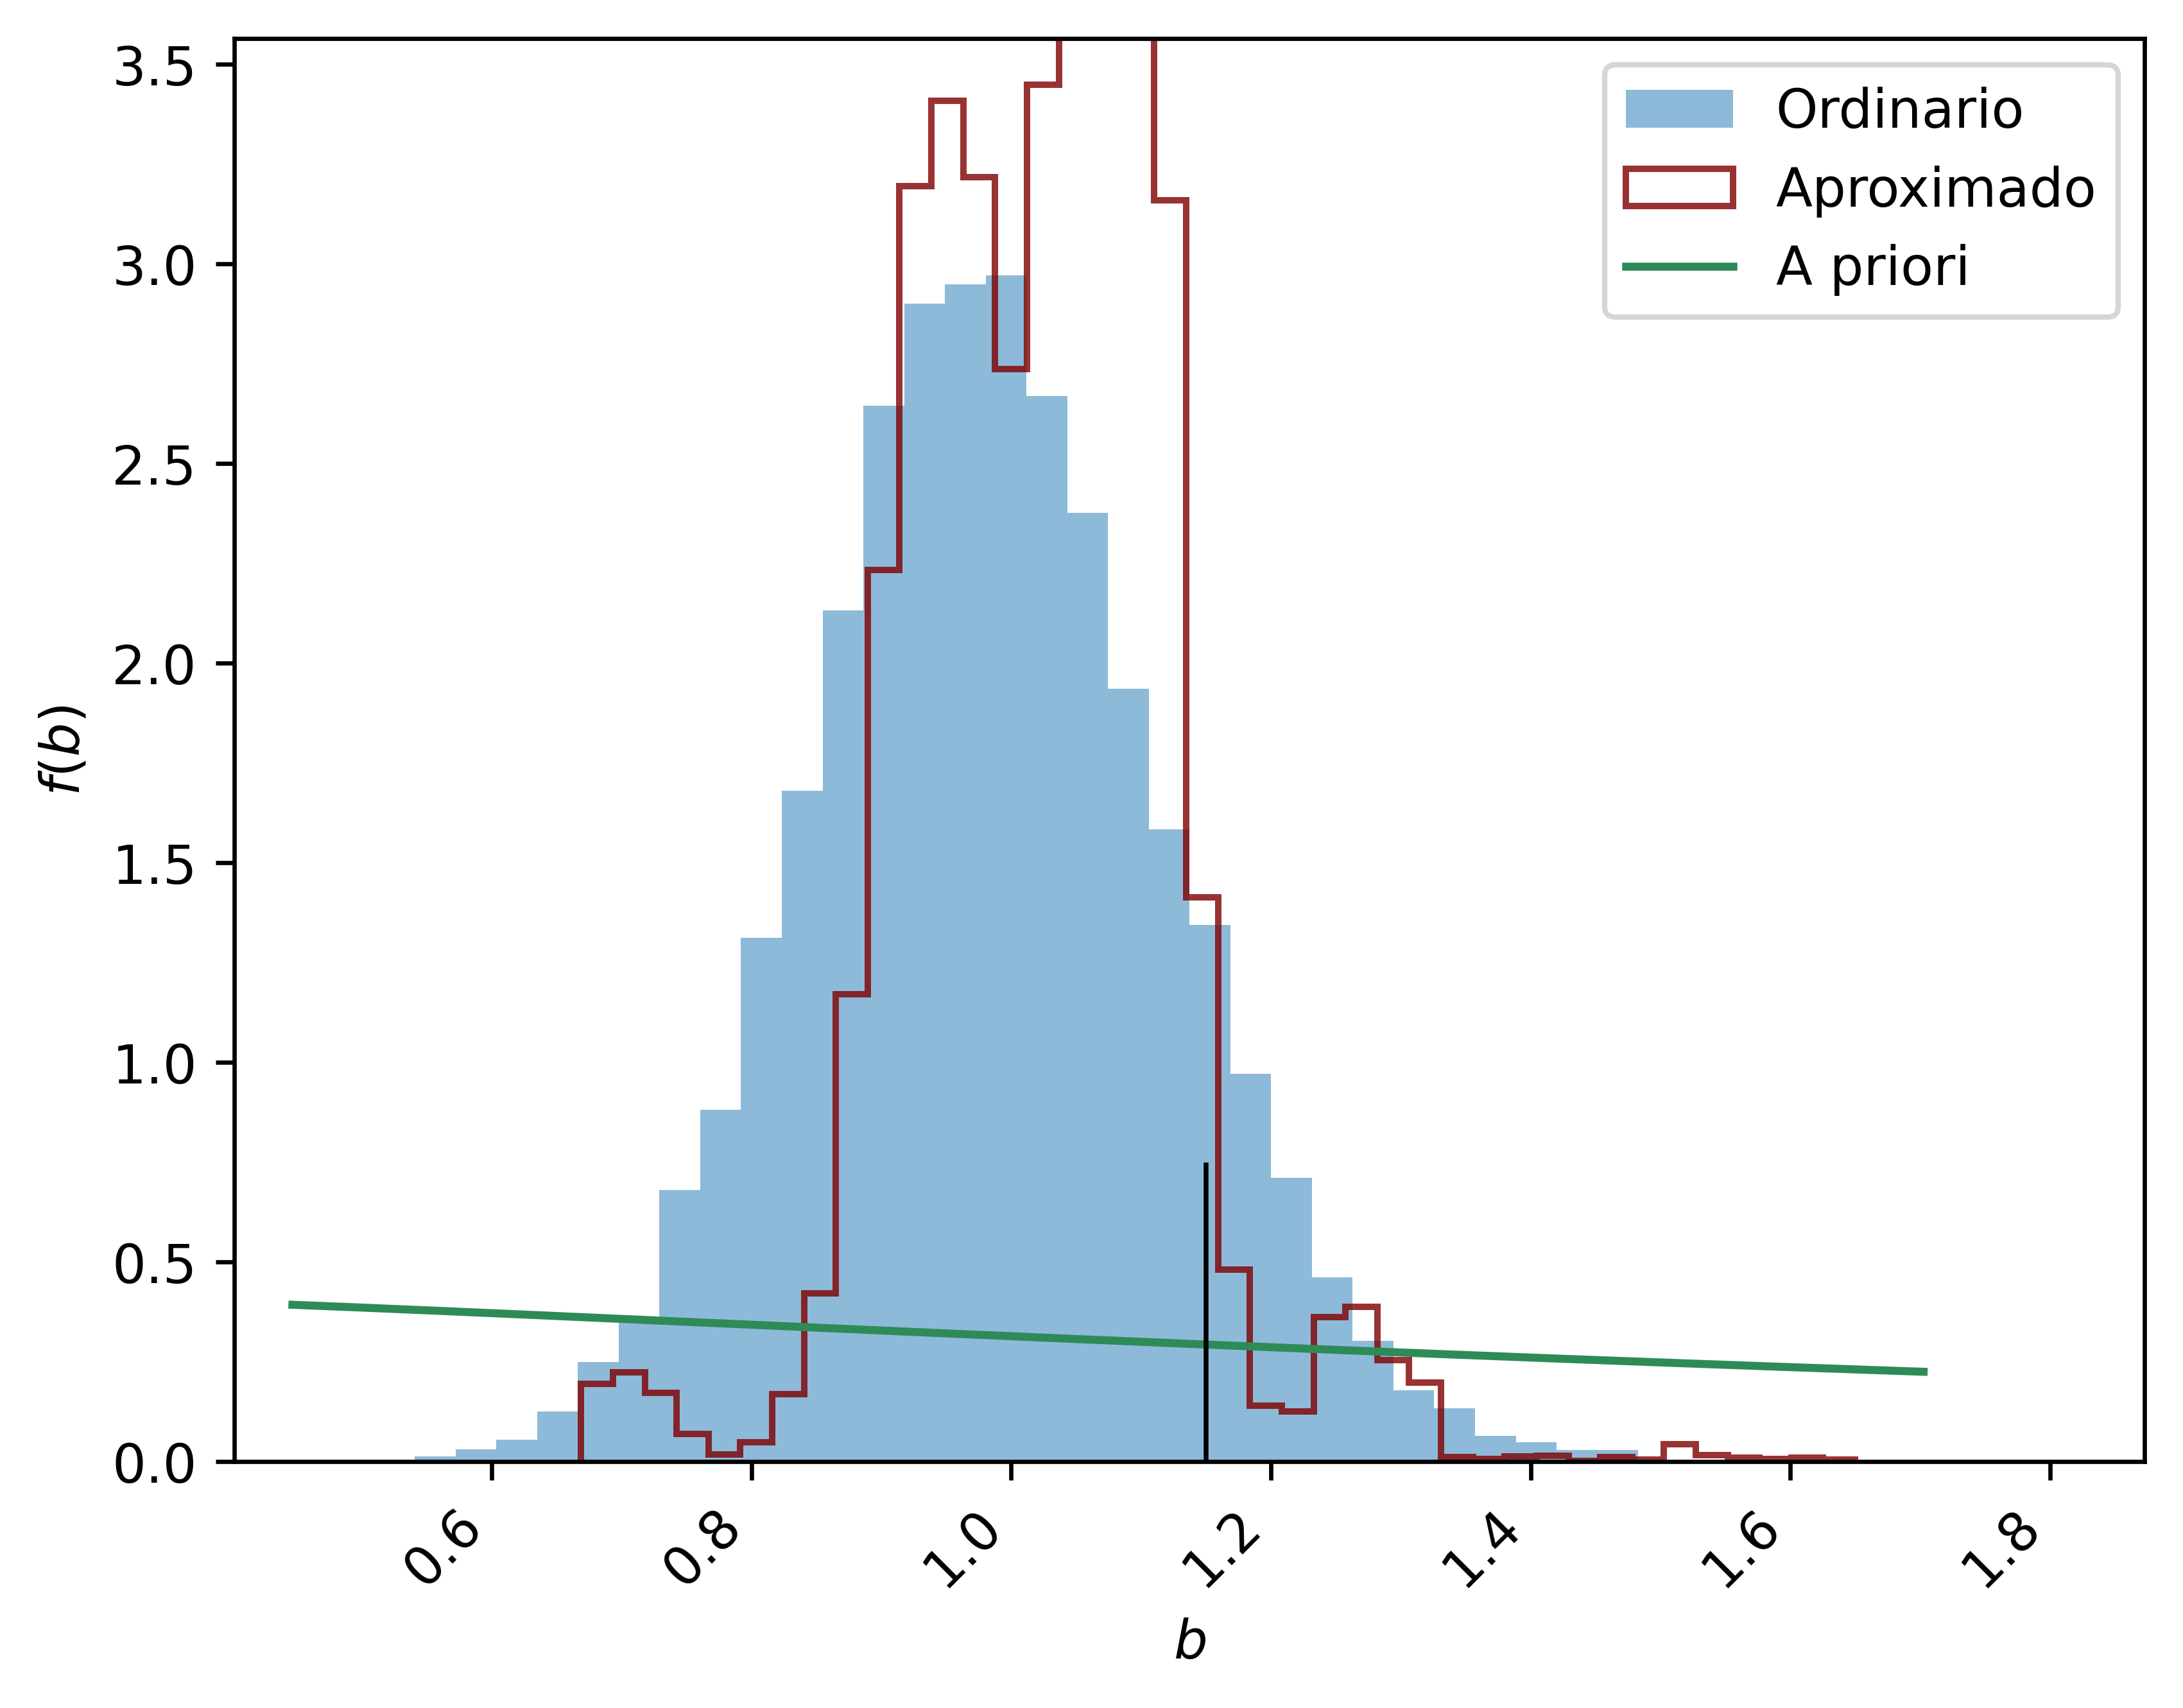
\includegraphics[width=0.4\textwidth]{img/Exp_Central_gravedad_sigma/Figuras/Individual/PostAprox_theta2_1_gravedad_sigma.png}
% %     \label{fig:subfig1}}
% %     \qquad
% %     \subfloat[Subfigure 2 list of figures text][Posterior con Forward aproximado en malla de 15x15]{
% %     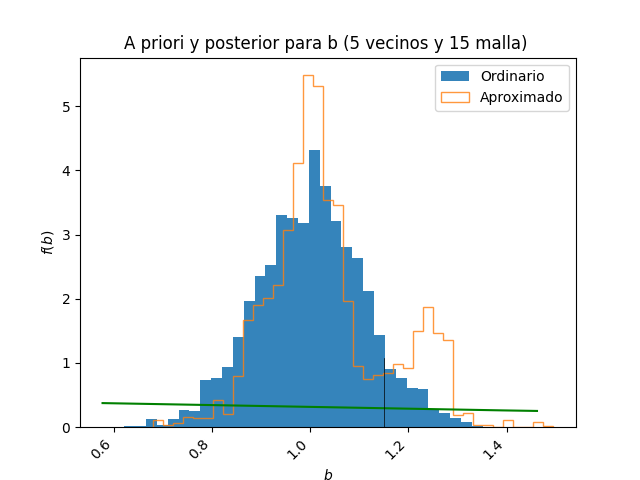
\includegraphics[width=0.4\textwidth]{img/Exp_Central_gravedad_sigma/Figuras/Individual/PostAprox_theta2_2_gravedad_sigma.png}
% %     \label{fig:subfig2}}
% %     \\
% %     \subfloat[Subfigure 3 list of figures text][Posterior con Forward aproximado en malla de 30x30]{
% %     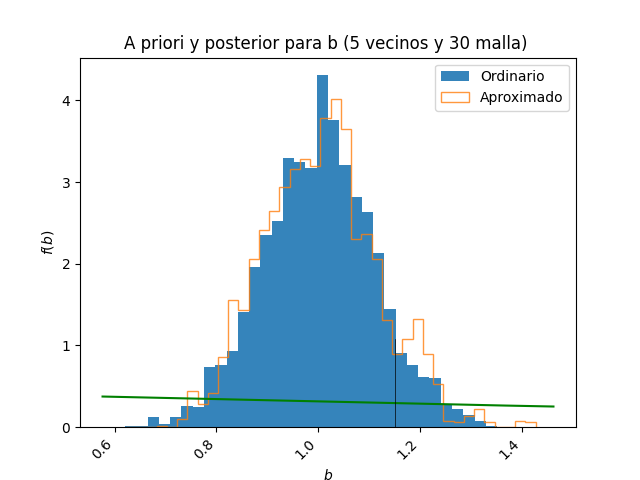
\includegraphics[width=0.4\textwidth]{img/Exp_Central_gravedad_sigma/Figuras/Individual/PostAprox_theta2_3_gravedad_sigma.png}
% %     \label{fig:subfig3}}
% %     \qquad
% %     \subfloat[Subfigure 4 list of figures text][Posterior con Forward aproximado en malla de 50x50]{
% %     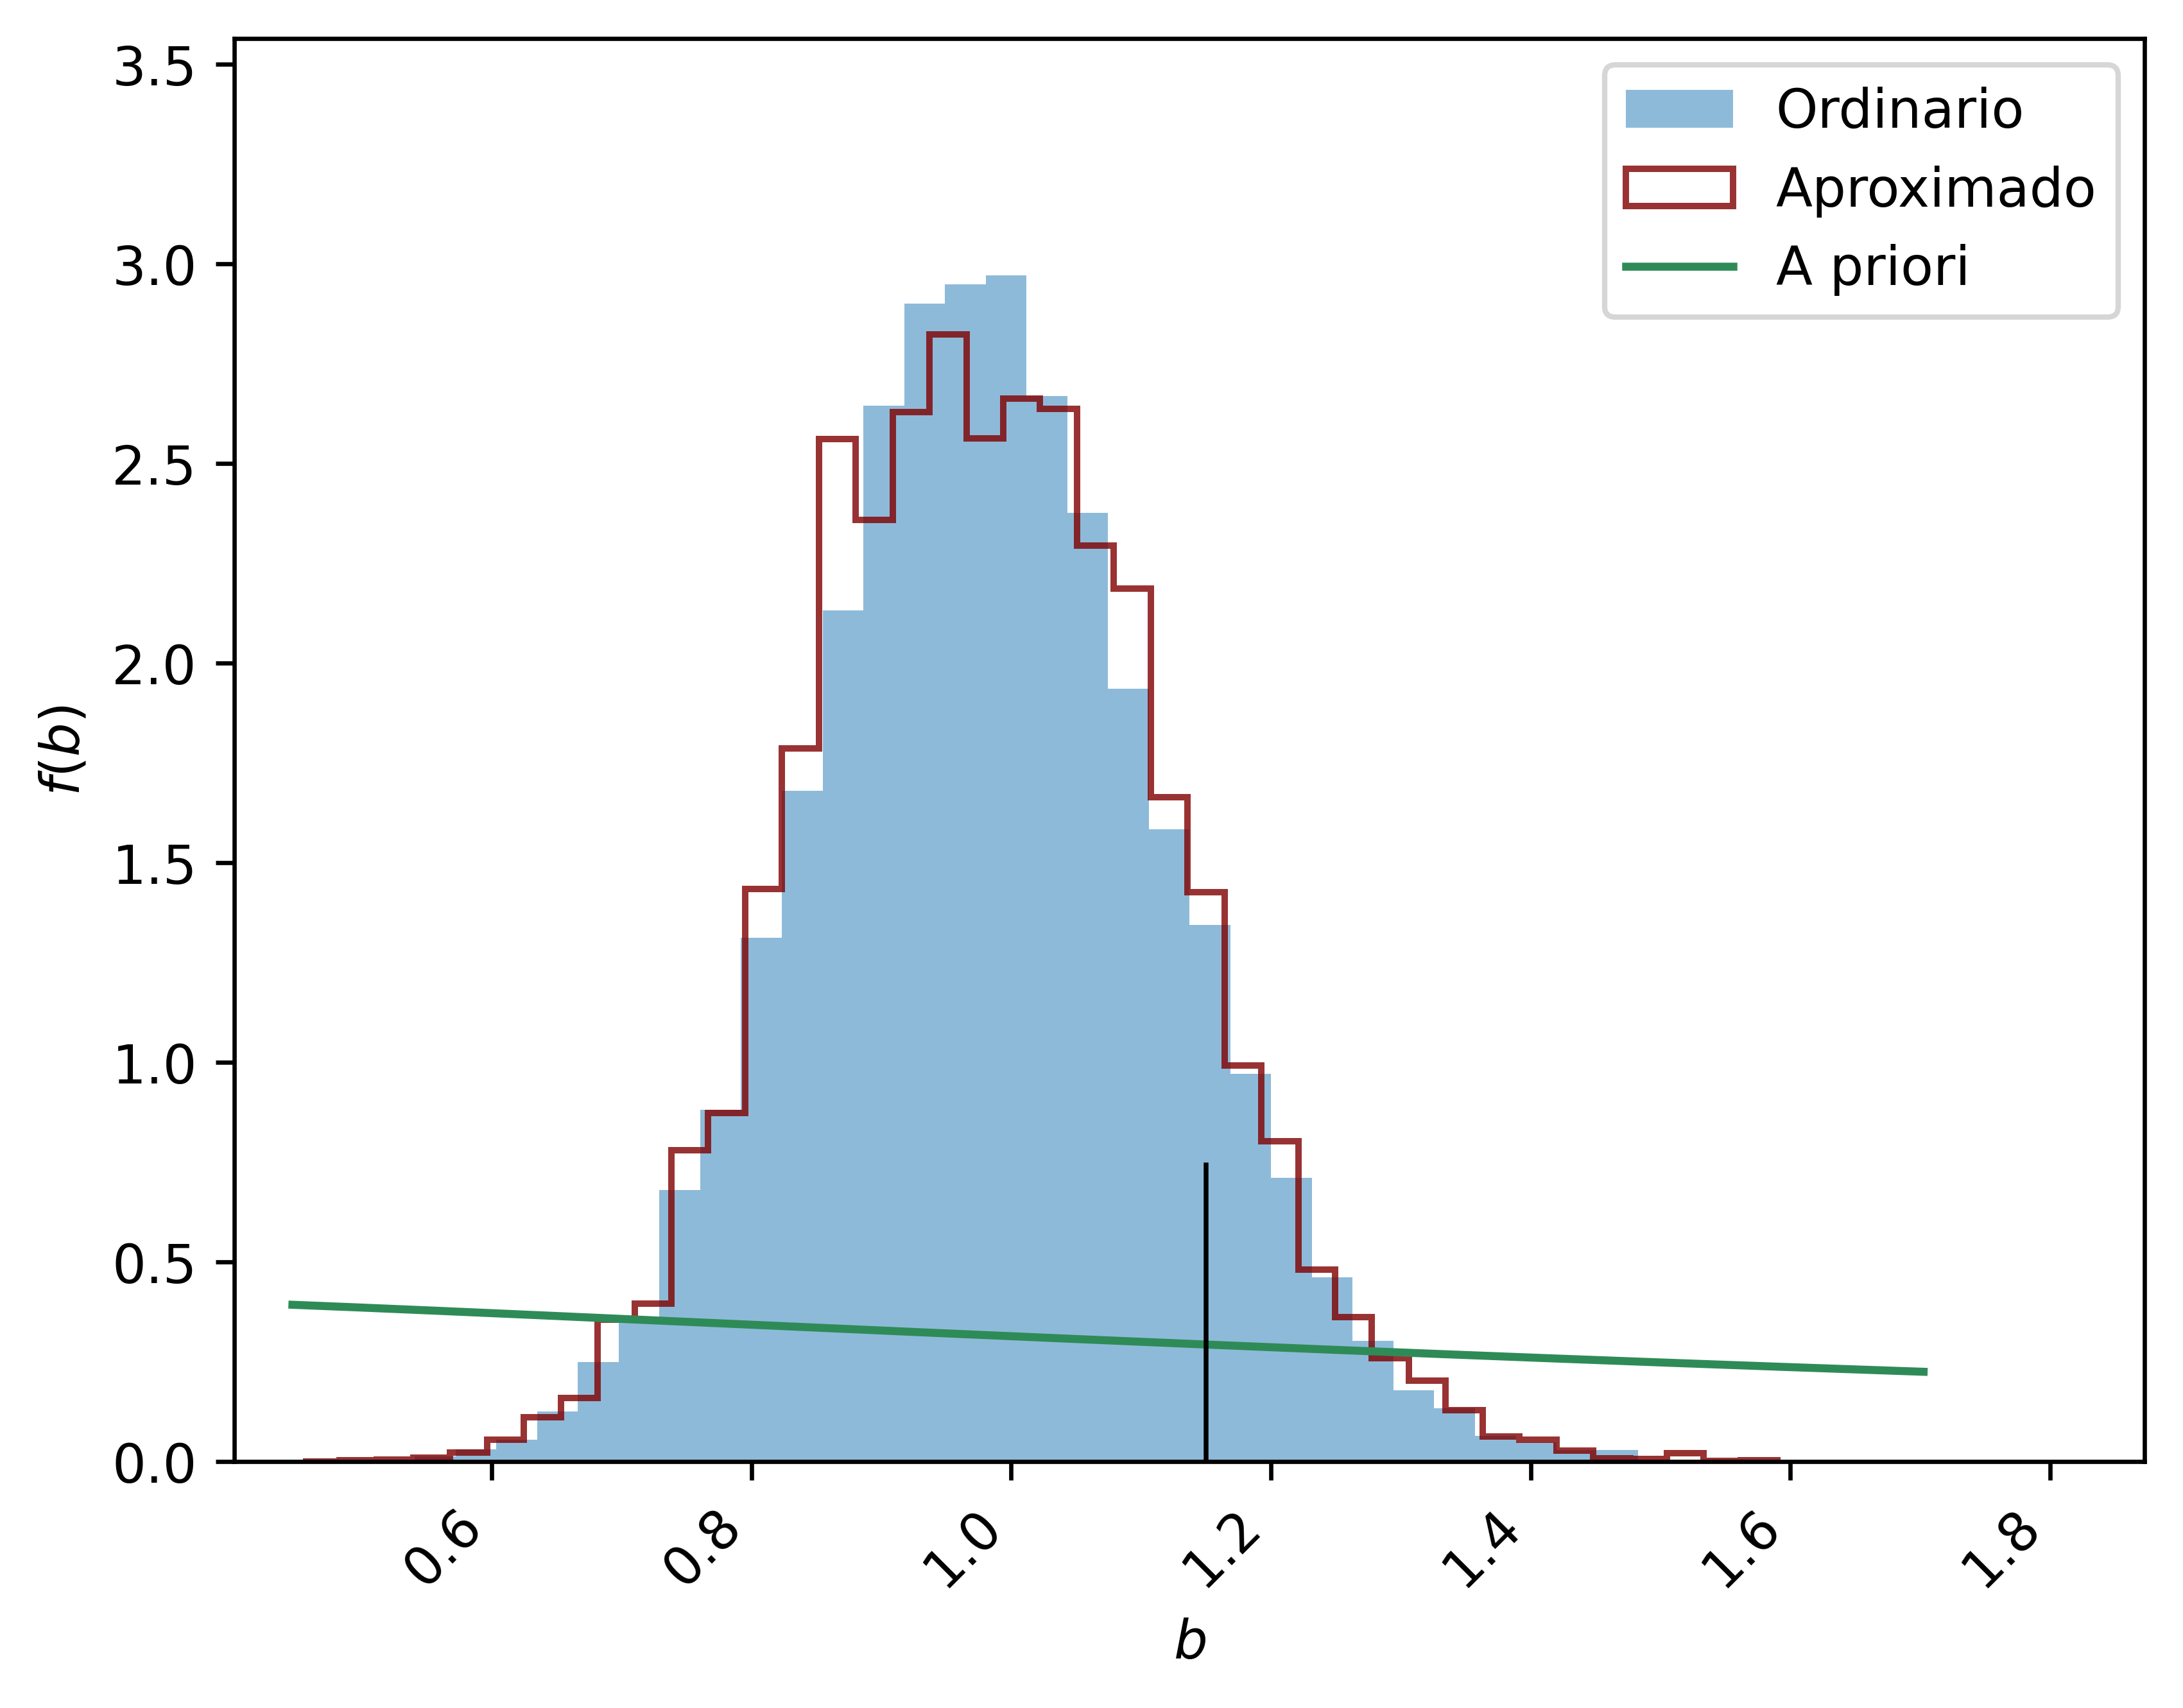
\includegraphics[width=0.4\textwidth]{img/Exp_Central_gravedad_sigma/Figuras/Individual/PostAprox_theta2_4_gravedad_sigma.png}
% %     \label{fig:subfig4}}
% %     \caption{Distribución posterior para $g$ con Forward ordinario y Forward aproximado con 5 vecinos cercanos.}
% %     \label{fig:g_01}
% % \end{figure}



% % \begin{figure}[h]
% %     \centering
% %     \subfloat[Subfigure 1 list of figures text][Posterior con Forward aproximado en malla de 10x10]{
% %     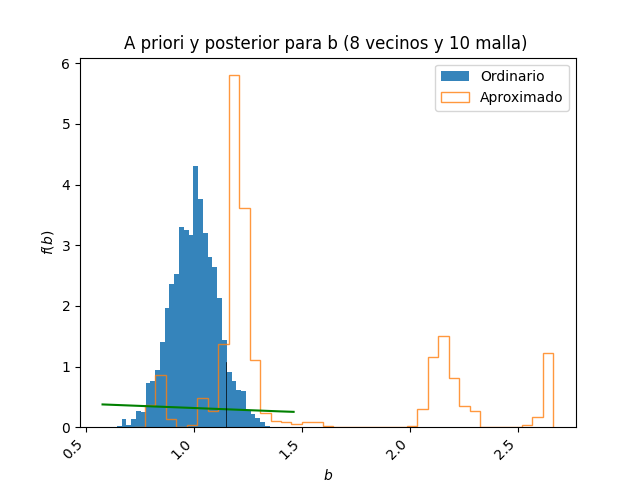
\includegraphics[width=0.4\textwidth]{img/Exp_Central_gravedad_sigma/Figuras/Individual/PostAprox_theta2_5_gravedad_sigma.png}
% %     \label{fig:subfig1}}
% %     \qquad
% %     \subfloat[Subfigure 2 list of figures text][Posterior con Forward aproximado en malla de 15x15]{
% %     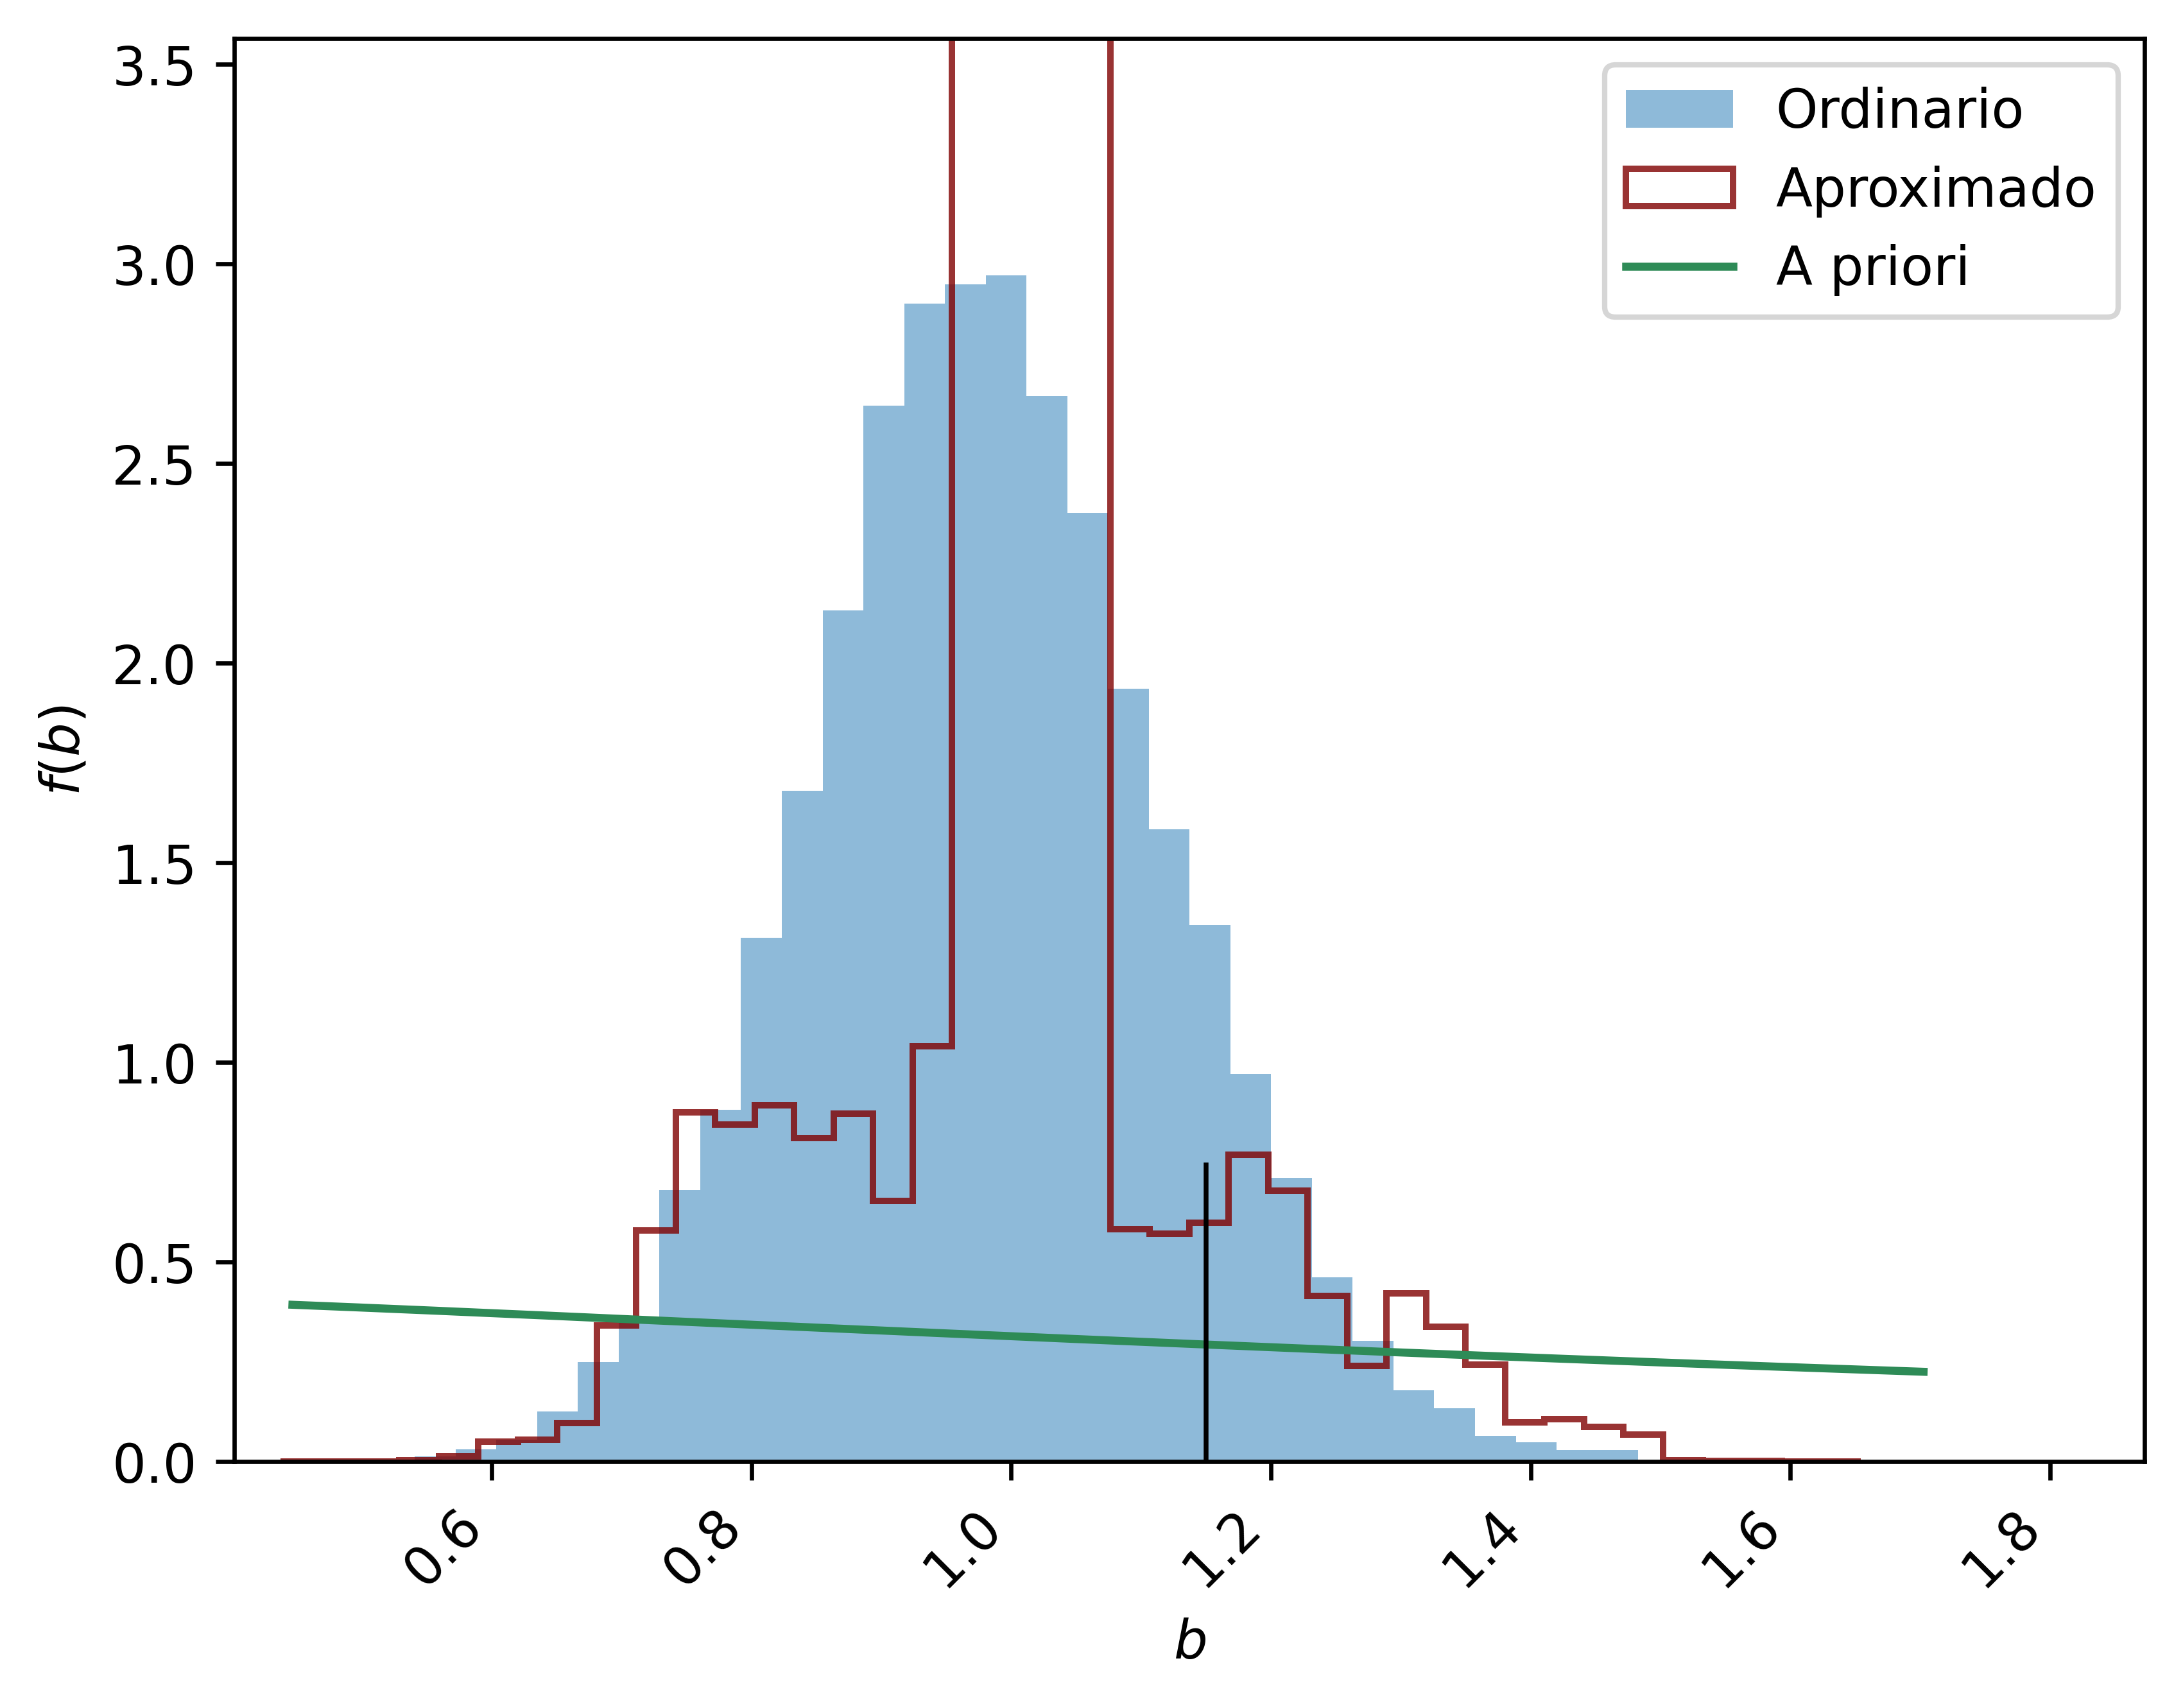
\includegraphics[width=0.4\textwidth]{img/Exp_Central_gravedad_sigma/Figuras/Individual/PostAprox_theta2_6_gravedad_sigma.png}
% %     \label{fig:subfig2}}
% %     \\
% %     \subfloat[Subfigure 3 list of figures text][Posterior con Forward aproximado en malla de 30x30]{
% %     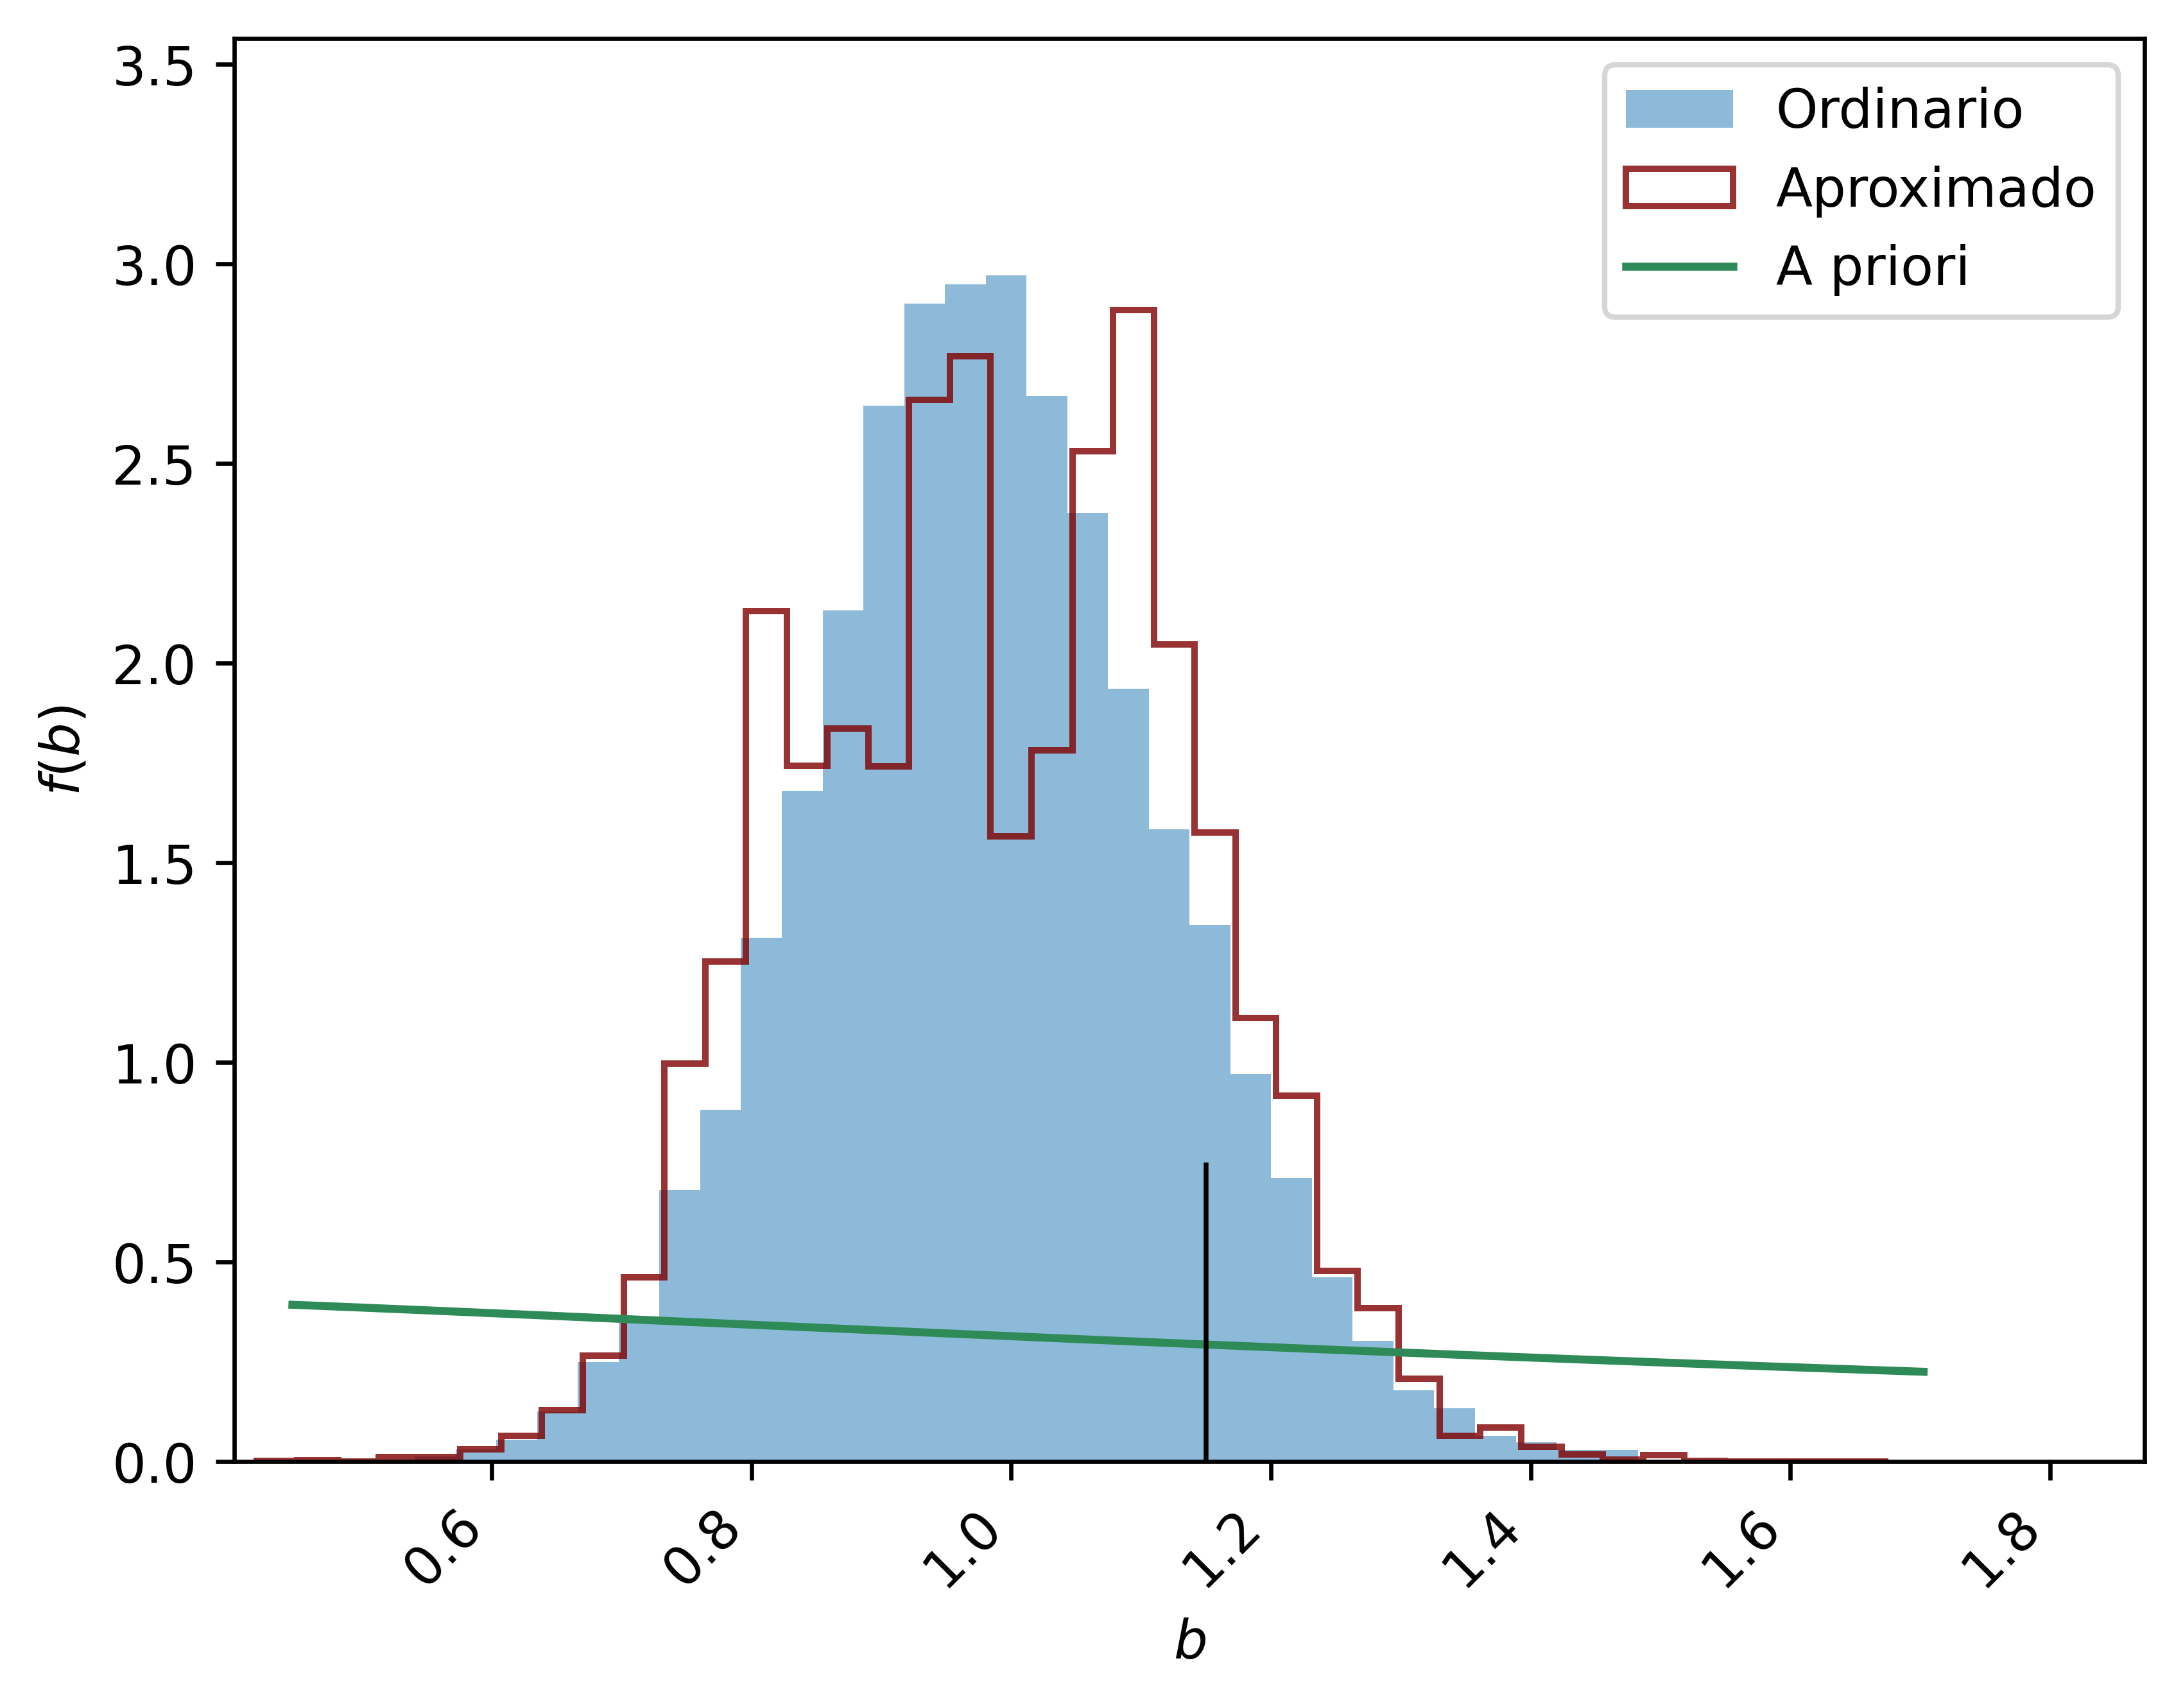
\includegraphics[width=0.4\textwidth]{img/Exp_Central_gravedad_sigma/Figuras/Individual/PostAprox_theta2_7_gravedad_sigma.png}
% %     \label{fig:subfig3}}
% %     \qquad
% %     \subfloat[Subfigure 4 list of figures text][Posterior con Forward aproximado en malla de 50x50]{
% %     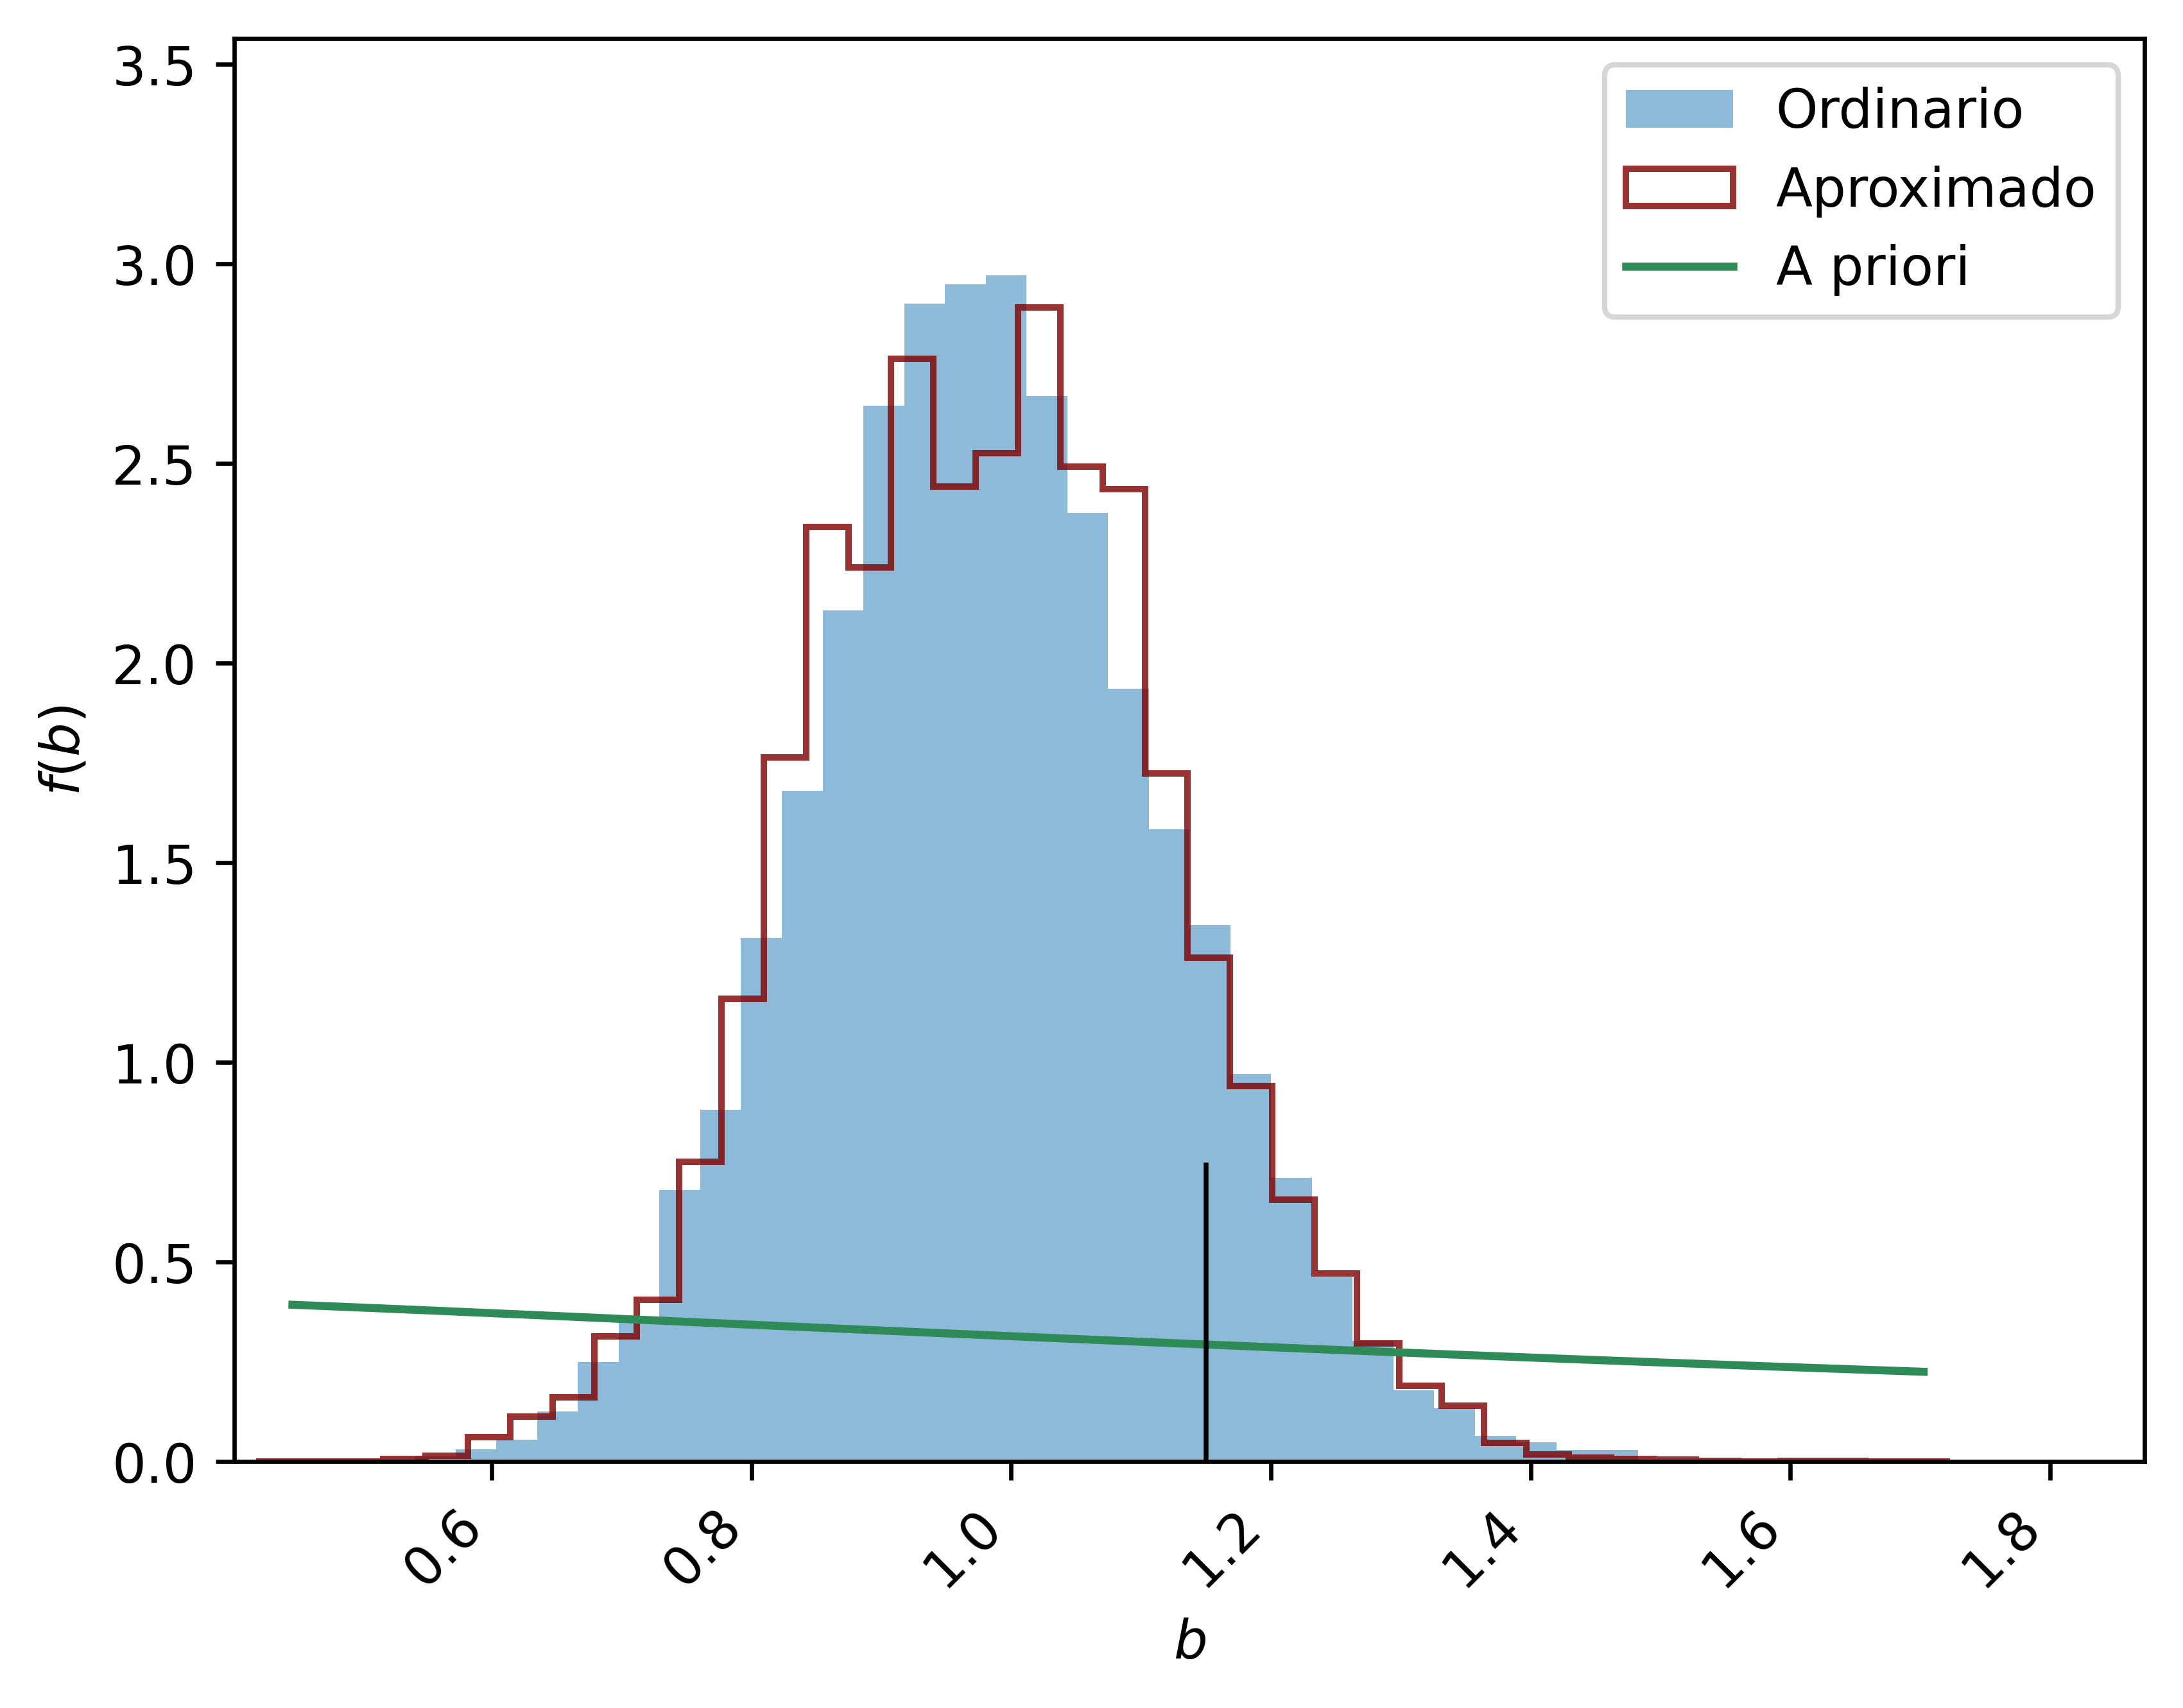
\includegraphics[width=0.4\textwidth]{img/Exp_Central_gravedad_sigma/Figuras/Individual/PostAprox_theta2_8_gravedad_sigma.png}
% %     \label{fig:subfig4}}
% %     \caption{Distribución posterior para $g$ con Forward ordinario y Forward aproximado con 5 vecinos cercanos.}
% %     \label{fig:g_01}
% % \end{figure}



% % \begin{figure}[h]
% %     \centering
% %     \subfloat[Subfigure 1 list of figures text][Posterior con Forward aproximado en malla de 10x10]{
% %     \includegraphics[width=0.4\textwidth]{img/Exp_Central_gravedad_sigma/Figuras/Individual/PostAprox_theta2_9_gravedad_sigma.png}
% %     \label{fig:subfig1}}
% %     \qquad
% %     \subfloat[Subfigure 2 list of figures text][Posterior con Forward aproximado en malla de 15x15]{
% %     \includegraphics[width=0.4\textwidth]{img/Exp_Central_gravedad_sigma/Figuras/Individual/PostAprox_theta2_10_gravedad_sigma.png}
% %     \label{fig:subfig2}}
% %     \\
% %     \subfloat[Subfigure 3 list of figures text][Posterior con Forward aproximado en malla de 30x30]{
% %     \includegraphics[width=0.4\textwidth]{img/Exp_Central_gravedad_sigma/Figuras/Individual/PostAprox_theta2_11_gravedad_sigma.png}
% %     \label{fig:subfig3}}
% %     \qquad
% %     \subfloat[Subfigure 4 list of figures text][Posterior con Forward aproximado en malla de 50x50]{
% %     \includegraphics[width=0.4\textwidth]{img/Exp_Central_gravedad_sigma/Figuras/Individual/PostAprox_theta2_12_gravedad_sigma.png}
% %     \label{fig:subfig4}}
% %     \caption{Distribución posterior para $g$ con Forward ordinario y Forward aproximado con 5 vecinos cercanos.}
% %     \label{fig:g_01}
% % \end{figure}

% \newpage

% \textbf{Forward map aproximado para el modelo logístico}











% En la Fig. () se muestran las distribuciones marginales para la aproximación del forward map con $k = 3$ y de izquierda a derecha una malla de 10x10, 15x15, 30x30, 50x50.

% \begin{figure}[H] 
%     \centering 
%     \includegraphics[width = 16 cm ]{img/Exp_Central_logistico_Sigma/Figuras/Generales/Convergencia_theta1_1_logistico_sigma.png} 
%     % \caption{}
%     % \label{Fig. }
% \end{figure} 

% \begin{figure}[H] 
%     \centering 
%     \includegraphics[width = 16 cm ]{img/Exp_Central_logistico_Sigma/Figuras/Generales/Convergencia_theta2_1_logistico_sigma.png} 
%     % \caption{}
%     % \label{Fig. }
% \end{figure} 

% En la Fig. () se muestran las distribuciones marginales para la aproximación del forward map con $k = 5$ y de izquierda a derecha una malla de 10x10, 15x15, 30x30, 50x50.

% \begin{figure}[H] 
%     \centering 
%     \includegraphics[width = 16 cm ]{img/Exp_Central_logistico_Sigma/Figuras/Generales/Convergencia_theta1_2_logistico_sigma.png} 
%     % \caption{}
%     % \label{Fig. }
% \end{figure} 

% \begin{figure}[H] 
%     \centering 
%     \includegraphics[width = 16 cm ]{img/Exp_Central_logistico_Sigma/Figuras/Generales/Convergencia_theta2_2_logistico_sigma.png} 
%     % \caption{}
%     % \label{Fig. }
% \end{figure} 

% En la Fig. () se muestran las distribuciones marginales para la aproximación del forward map con $k = 8$ y de izquierda a derecha una malla de 10x10, 15x15, 30x30, 50x50.

% \begin{figure}[H] 
%     \centering 
%     \includegraphics[width = 16 cm ]{img/Exp_Central_logistico_Sigma/Figuras/Generales/Convergencia_theta1_3_logistico_sigma.png} 
%     % \caption{}
%     % \label{Fig. }
% \end{figure} 

% \begin{figure}[H] 
%     \centering 
%     \includegraphics[width = 16 cm ]{img/Exp_Central_logistico_Sigma/Figuras/Generales/Convergencia_theta2_3_logistico_sigma.png} 
%     % \caption{}
%     % \label{Fig. }
% \end{figure} 



% El tiempo de ejecución del método ordinario para el problema inverso en el modelo logístico es de \textbf{20 min 58 s}


% \begin{table}[H]
%     \centering
%     \begin{tabular}{l r r r c}
%       \toprule
%        \textbf{Malla} & \textbf{\:\:\:\:\:\:\:10 x 10\:\:\:\:\:\:\:} & \textbf{\:\:\:\:\:\:\:15 x 15\:\:\:\:\:\:\:} & \textbf{\:\:\:\:\:\:\:30 x 30\:\:\:\:\:\:\:} & \textbf{\:\:\:\:\:\:\:50 x 50\:\:\:\:\:\:\:} \\
%       \midrule
%       3 vecinos & 10m 58s & 9m 36s & 9m 25s & \textbf{6m 02s}\\
%       5 vecinos & 6m 02s & 6m 03s & 7m 20s & 10m 04s\\
%       8 vecinos & 10m 08s & 10m 24s & 10m 21s & 10m 21s\\
%       \bottomrule
%     \end{tabular}
%     % \caption{A table caption.}
%     % \label{tabla_03}
% \end{table}


















































% % \begin{figure}[h]
% %     \centering
% %     \subfloat[Subfigure 1 list of figures text][Posterior con Forward aproximado en malla de 10x10]{
% %     \includegraphics[width=0.4\textwidth]{img/Exp_Central_logistico/Figuras/Individual/PostAprox_theta1_1_logistico.png}
% %     \label{fig:subfig1}}
% %     \qquad
% %     \subfloat[Subfigure 2 list of figures text][Posterior con Forward aproximado en malla de 15x15]{
% %     \includegraphics[width=0.4\textwidth]{img/Exp_Central_logistico/Figuras/Individual/PostAprox_theta1_2_logistico.png}
% %     \label{fig:subfig2}}
% %     \\
% %     \subfloat[Subfigure 3 list of figures text][Posterior con Forward aproximado en malla de 30x30]{
% %     \includegraphics[width=0.4\textwidth]{img/Exp_Central_logistico/Figuras/Individual/PostAprox_theta1_3_logistico.png}
% %     \label{fig:subfig3}}
% %     \qquad
% %     \subfloat[Subfigure 4 list of figures text][Posterior con Forward aproximado en malla de 50x50]{
% %     \includegraphics[width=0.4\textwidth]{img/Exp_Central_logistico/Figuras/Individual/PostAprox_theta1_4_logistico.png}
% %     \label{fig:subfig4}}
% %     \caption{Distribución posterior para $g$ con Forward ordinario y Forward aproximado con 5 vecinos cercanos.}
% %     \label{fig:g_01}
% % \end{figure}


% % \begin{figure}[h]
% %     \centering
% %     \subfloat[Subfigure 1 list of figures text][Posterior con Forward aproximado en malla de 10x10]{
% %     \includegraphics[width=0.4\textwidth]{img/Exp_Central_logistico/Figuras/Individual/PostAprox_theta1_5_logistico.png}
% %     \label{fig:subfig1}}
% %     \qquad
% %     \subfloat[Subfigure 2 list of figures text][Posterior con Forward aproximado en malla de 15x15]{
% %     \includegraphics[width=0.4\textwidth]{img/Exp_Central_logistico/Figuras/Individual/PostAprox_theta1_6_logistico.png}
% %     \label{fig:subfig2}}
% %     \\
% %     \subfloat[Subfigure 3 list of figures text][Posterior con Forward aproximado en malla de 30x30]{
% %     \includegraphics[width=0.4\textwidth]{img/Exp_Central_logistico/Figuras/Individual/PostAprox_theta1_7_logistico.png}
% %     \label{fig:subfig3}}
% %     \qquad
% %     \subfloat[Subfigure 4 list of figures text][Posterior con Forward aproximado en malla de 50x50]{
% %     \includegraphics[width=0.4\textwidth]{img/Exp_Central_logistico/Figuras/Individual/PostAprox_theta1_8_logistico.png}
% %     \label{fig:subfig4}}
% %     \caption{Distribución posterior para $g$ con Forward ordinario y Forward aproximado con 5 vecinos cercanos.}
% %     \label{fig:g_01}
% % \end{figure}


% % \begin{figure}[h]
% %     \centering
% %     \subfloat[Subfigure 1 list of figures text][Posterior con Forward aproximado en malla de 10x10]{
% %     \includegraphics[width=0.4\textwidth]{img/Exp_Central_logistico/Figuras/Individual/PostAprox_theta1_9_logistico.png}
% %     \label{fig:subfig1}}
% %     \qquad
% %     \subfloat[Subfigure 2 list of figures text][Posterior con Forward aproximado en malla de 15x15]{
% %     \includegraphics[width=0.4\textwidth]{img/Exp_Central_logistico/Figuras/Individual/PostAprox_theta1_10_logistico.png}
% %     \label{fig:subfig2}}
% %     \\
% %     \subfloat[Subfigure 3 list of figures text][Posterior con Forward aproximado en malla de 30x30]{
% %     \includegraphics[width=0.4\textwidth]{img/Exp_Central_logistico/Figuras/Individual/PostAprox_theta1_11_logistico.png}
% %     \label{fig:subfig3}}
% %     \qquad
% %     \subfloat[Subfigure 4 list of figures text][Posterior con Forward aproximado en malla de 50x50]{
% %     \includegraphics[width=0.4\textwidth]{img/Exp_Central_logistico/Figuras/Individual/PostAprox_theta1_12_logistico.png}
% %     \label{fig:subfig4}}
% %     \caption{Distribución posterior para $g$ con Forward ordinario y Forward aproximado con 5 vecinos cercanos.}
% %     \label{fig:g_01}
% % \end{figure}




% % \begin{figure}[h]
% %     \centering
% %     \subfloat[Subfigure 1 list of figures text][Posterior con Forward aproximado en malla de 10x10]{
% %     \includegraphics[width=0.4\textwidth]{img/Exp_Central_logistico/Figuras/Individual/PostAprox_theta2_1_logistico.png}
% %     \label{fig:subfig1}}
% %     \qquad
% %     \subfloat[Subfigure 2 list of figures text][Posterior con Forward aproximado en malla de 15x15]{
% %     \includegraphics[width=0.4\textwidth]{img/Exp_Central_logistico/Figuras/Individual/PostAprox_theta2_2_logistico.png}
% %     \label{fig:subfig2}}
% %     \\
% %     \subfloat[Subfigure 3 list of figures text][Posterior con Forward aproximado en malla de 30x30]{
% %     \includegraphics[width=0.4\textwidth]{img/Exp_Central_logistico/Figuras/Individual/PostAprox_theta2_3_logistico.png}
% %     \label{fig:subfig3}}
% %     \qquad
% %     \subfloat[Subfigure 4 list of figures text][Posterior con Forward aproximado en malla de 50x50]{
% %     \includegraphics[width=0.4\textwidth]{img/Exp_Central_logistico/Figuras/Individual/PostAprox_theta2_4_logistico.png}
% %     \label{fig:subfig4}}
% %     \caption{Distribución posterior para $g$ con Forward ordinario y Forward aproximado con 5 vecinos cercanos.}
% %     \label{fig:g_01}
% % \end{figure}



% % \begin{figure}[h]
% %     \centering
% %     \subfloat[Subfigure 1 list of figures text][Posterior con Forward aproximado en malla de 10x10]{
% %     \includegraphics[width=0.4\textwidth]{img/Exp_Central_logistico/Figuras/Individual/PostAprox_theta2_5_logistico.png}
% %     \label{fig:subfig1}}
% %     \qquad
% %     \subfloat[Subfigure 2 list of figures text][Posterior con Forward aproximado en malla de 15x15]{
% %     \includegraphics[width=0.4\textwidth]{img/Exp_Central_logistico/Figuras/Individual/PostAprox_theta2_6_logistico.png}
% %     \label{fig:subfig2}}
% %     \\
% %     \subfloat[Subfigure 3 list of figures text][Posterior con Forward aproximado en malla de 30x30]{
% %     \includegraphics[width=0.4\textwidth]{img/Exp_Central_logistico/Figuras/Individual/PostAprox_theta2_7_logistico.png}
% %     \label{fig:subfig3}}
% %     \qquad
% %     \subfloat[Subfigure 4 list of figures text][Posterior con Forward aproximado en malla de 50x50]{
% %     \includegraphics[width=0.4\textwidth]{img/Exp_Central_logistico/Figuras/Individual/PostAprox_theta2_8_logistico.png}
% %     \label{fig:subfig4}}
% %     \caption{Distribución posterior para $g$ con Forward ordinario y Forward aproximado con 5 vecinos cercanos.}
% %     \label{fig:g_01}
% % \end{figure}



% % \begin{figure}[h]
% %     \centering
% %     \subfloat[Subfigure 1 list of figures text][Posterior con Forward aproximado en malla de 10x10]{
% %     \includegraphics[width=0.4\textwidth]{img/Exp_Central_logistico/Figuras/Individual/PostAprox_theta2_9_logistico.png}
% %     \label{fig:subfig1}}
% %     \qquad
% %     \subfloat[Subfigure 2 list of figures text][Posterior con Forward aproximado en malla de 15x15]{
% %     \includegraphics[width=0.4\textwidth]{img/Exp_Central_logistico/Figuras/Individual/PostAprox_theta2_10_logistico.png}
% %     \label{fig:subfig2}}
% %     \\
% %     \subfloat[Subfigure 3 list of figures text][Posterior con Forward aproximado en malla de 30x30]{
% %     \includegraphics[width=0.4\textwidth]{img/Exp_Central_logistico/Figuras/Individual/PostAprox_theta2_11_logistico.png}
% %     \label{fig:subfig3}}
% %     \qquad
% %     \subfloat[Subfigure 4 list of figures text][Posterior con Forward aproximado en malla de 50x50]{
% %     \includegraphics[width=0.4\textwidth]{img/Exp_Central_logistico/Figuras/Individual/PostAprox_theta2_12_logistico.png}
% %     \label{fig:subfig4}}
% %     \caption{Distribución posterior para $g$ con Forward ordinario y Forward aproximado con 5 vecinos cercanos.}
% %     \label{fig:g_01}
% % \end{figure}

% \newpage

% \newpage

% \newpage

% \newpage


% \subsubsection{Convergencia en el modelo epidemiólogico}

% El problema inverso en el modelo SIR se observa la relevancia de la aproximación del forward map. Recordemos que el forward map del modelo SIR no es posible obtenerse de manera analítica, lo que conlleva un consumo computacional añadido al momento de analizar los pormenores. Una dificultad para el forward map aproximado radica en el gran cambio de unidades, puesto que las unidades entre los parámetros $\beta$ y $\gamma$ difieren por un orden de magnitud, lo que es necesario del ajuste al espacio de parámetros. 


% % Haciendo repetidas inferencias con distintas aproximaciones. Esto es tomar forward maps que consideren 3, 5, 8 vecinos cercanos con cubrimiento de malla desde $10 x 10, 15x15, 30x30, 50x50$. Al igual que los casos anteriores los tiempos de ejecución en cada caso se dan en la table (\ref{tabla_03})





% En la Fig. () se muestran las distribuciones marginales para la aproximación del forward map con $k = 5$ y de izquierda a derecha una malla de 10x10, 15x15, 30x30, 50x50.


% \begin{figure}[H] 
%     \centering 
%     \includegraphics[width = 17 cm ]{img/Exp_Central_SIR_Sigma/Figuras/Generales/Convergencia_theta1_1_SIR_sigma.png} 
%     % \caption{}
%     % \label{Fig. }
% \end{figure} 

% \begin{figure}[H] 
%     \centering 
%     \includegraphics[width = 17 cm ]{img/Exp_Central_SIR_Sigma/Figuras/Generales/Convergencia_theta1_2_SIR_sigma.png} 
%     % \caption{}
%     % \label{Fig. }
% \end{figure} 

% En la Fig. () se muestran las distribuciones marginales para la aproximación del forward map con $k = 5$ y de izquierda a derecha una malla de 10x10, 15x15, 30x30, 50x50.

% \begin{figure}[H] 
%     \centering 
%     \includegraphics[width = 17 cm ]{img/Exp_Central_SIR_Sigma/Figuras/Generales/Convergencia_theta1_3_SIR_sigma.png} 
%     % \caption{}
%     % \label{Fig. }
% \end{figure} 

% \begin{figure}[H] 
%     \centering 
%     \includegraphics[width = 17 cm ]{img/Exp_Central_SIR_Sigma/Figuras/Generales/Convergencia_theta2_1_SIR_sigma.png} 
%     % \caption{}
%     % \label{Fig. }
% \end{figure} 

% En la Fig. () se muestran las distribuciones marginales para la aproximación del forward map con $k = 5$ y de izquierda a derecha una malla de 10x10, 15x15, 30x30, 50x50.

% \begin{figure}[H] 
%     \centering 
%     \includegraphics[width = 17 cm ]{img/Exp_Central_SIR_Sigma/Figuras/Generales/Convergencia_theta2_2_SIR_sigma.png} 
%     % \caption{}
%     % \label{Fig. }
% \end{figure} 

% \begin{figure}[H] 
%     \centering 
%     \includegraphics[width = 17 cm ]{img/Exp_Central_SIR_Sigma/Figuras/Generales/Convergencia_theta2_3_SIR_sigma.png} 
%     % \caption{}
%     % \label{Fig. }
% \end{figure} 


% El tiempo de ejecución del método ordinario para el problema inverso en el modelo gravitacional es de \textbf{14 min 05 seg}


% \begin{table}[H]
%     \centering
%     \begin{tabular}{l r r r c}
%       \toprule
%        \textbf{Malla} & \textbf{\:\:\:\:\:\:\:10 x 10\:\:\:\:\:\:\:} & \textbf{\:\:\:\:\:\:\:15 x 15\:\:\:\:\:\:\:} & \textbf{\:\:\:\:\:\:\:30 x 30\:\:\:\:\:\:\:} & \textbf{\:\:\:\:\:\:\:50 x 50\:\:\:\:\:\:\:} \\
%       \midrule
%       3 vecinos & 5m 38s & 5m 36s & 8m 14s & \textbf{5m 50s}\\
%       5 vecinos & 5m 59s & 5m 50s & 5m 56s & 5m 57s\\
%       8 vecinos & 6m 38s & 7m 26s & 7m 02s & 6m 09s\\
%       \bottomrule
%     \end{tabular}
%     % \caption{A table caption.}
%     % \label{tabla_03}
% \end{table}















% % \begin{figure}
% %     \centering
% %     \includegraphics{img/posterior_g_1.png}
% %     \caption{Caption}
% %     \label{fig:enter-label}
% % \end{figure}


% % \begin{figure}
% % \begin{subfigure}{.5\textwidth}
% %   \centering
% %   \includegraphics[width=.8\linewidth]{img/posterior_g_1.png}
% %   \caption{1}
% %   \label{fig:sfig2}
% % \end{subfigure}
% % \begin{subfigure}{.5\textwidth}
% %   \centering
% %   \includegraphics[width=.8\linewidth]{img/posterior_g_2.png}
% %   \caption{2}
% %   \label{fig:sfig1}
% % \end{subfigure}%
% % \begin{subfigure}{.5\textwidth}
% %   \centering
% %   \includegraphics[width=.8\linewidth]{img/posterior_g_3.png}
% %   \caption{3}
% %   \label{fig:sfig2}
% % \end{subfigure}
% % \begin{subfigure}{.5\textwidth}
% %   \centering
% %   \includegraphics[width=.8\linewidth]{img/posterior_g_4.png}
% %   \caption{4}
% %   \label{fig:sfig2}
% % \end{subfigure}
% % \caption{plots of....}
% % \label{fig:fig}
% % \end{figure}

% % % 5 vecinos
% % \begin{figure}[h]
% %     \centering
% %     \subfloat[Subfigure 1 list of figures text][Posterior con Forward aproximado en malla de 10x10]{
% %     \includegraphics[width=0.4\textwidth]{img/posterior_g_1.png}
% %     \label{fig:subfig1}}
% %     \qquad
% %     \subfloat[Subfigure 2 list of figures text][Posterior con Forward aproximado en malla de 15x15]{
% %     \includegraphics[width=0.4\textwidth]{img/posterior_g_2.png}
% %     \label{fig:subfig2}}\\
% %     \subfloat[Subfigure 3 list of figures text][Posterior con Forward aproximado en malla de 30x30]{
% %     \includegraphics[width=0.4\textwidth]{img/posterior_g_3.png}
% %     \label{fig:subfig3}}
% %     \qquad
% %     \subfloat[Subfigure 4 list of figures text][Posterior con Forward aproximado en malla de 50x50]{
% %     \includegraphics[width=0.4\textwidth]{img/posterior_g_4.png}
% %     \label{fig:subfig4}}
% %     \caption{Distribución posterior para $g$ con Forward ordinario y Forward aproximado con 5 vecinos cercanos.}
% %     \label{fig:g_01}
% % \end{figure}


% % % 8 vecinos
% % \begin{figure}[h]
% %     \centering
% %     \subfloat[Subfigure 1 list of figures text][Posterior con Forward aproximado en malla de 10x10]{
% %     \includegraphics[width=0.4\textwidth]{img/posterior_g_5.png}
% %     \label{fig:subfig1}}
% %     \qquad
% %     \subfloat[Subfigure 2 list of figures text][Posterior con Forward aproximado en malla de 15x15]{
% %     \includegraphics[width=0.4\textwidth]{img/posterior_g_6.png}
% %     \label{fig:subfig2}}
% %     \subfloat[Subfigure 3 list of figures text][Posterior con Forward aproximado en malla de 30x30]{
% %     \includegraphics[width=0.4\textwidth]{img/posterior_g_7.png}
% %     \label{fig:subfig3}}
% %     \qquad
% %     \subfloat[Subfigure 4 list of figures text][Posterior con Forward aproximado en malla de 50x50]{
% %     \includegraphics[width=0.4\textwidth]{img/posterior_g_8.png}
% %     \label{fig:subfig4}}
% %     \caption{Distribución posterior para $g$ con Forward ordinario y Forward aproximado con 8 vecinos cercanos.}
% %     \label{fig:g_02}
% % \end{figure}


% % % 16 vecinos
% % \begin{figure}[h]
% %     \centering
% %     \subfloat[Subfigure 1 list of figures text][Posterior con Forward aproximado en malla de 10x10]{
% %     \includegraphics[width=0.4\textwidth]{img/posterior_g_9.png}
% %     \label{fig:subfig1}}
% %     \qquad
% %     \subfloat[Subfigure 2 list of figures text][Posterior con Forward aproximado en malla de 15x15]{
% %     \includegraphics[width=0.4\textwidth]{img/posterior_g_10.png}
% %     \label{fig:subfig2}}
% %     \subfloat[Subfigure 3 list of figures text][Posterior con Forward aproximado en malla de 30x30]{
% %     \includegraphics[width=0.4\textwidth]{img/posterior_g_11.png}
% %     \label{fig:subfig3}}
% %     \qquad
% %     \subfloat[Subfigure 4 list of figures text][Posterior con Forward aproximado en malla de 50x50]{
% %     \includegraphics[width=0.4\textwidth]{img/posterior_g_12.png}
% %     \label{fig:subfig4}}
% %     \caption{Distribución posterior para $g$ con Forward ordinario y Forward aproximado con 16 vecinos cercanos.}
% %     \label{fig:g_03}
% % \end{figure}



% % Para el otro parámetro $b$ tenemos las siguientes posteriores

% % % 5 vecinos
% % \begin{figure}[h]
% %     \centering
% %     \subfloat[Subfigure 1 list of figures text][Posterior con Forward aproximado en malla de 10x10]{
% %     \includegraphics[width=0.4\textwidth]{img/posterior_b_1.png}
% %     \label{fig:subfig1}}
% %     \qquad
% %     \subfloat[Subfigure 2 list of figures text][Posterior con Forward aproximado en malla de 15x15]{
% %     \includegraphics[width=0.4\textwidth]{img/posterior_b_2.png}
% %     \label{fig:subfig2}}
% %     \subfloat[Subfigure 3 list of figures text][Posterior con Forward aproximado en malla de 30x30]{
% %     \includegraphics[width=0.4\textwidth]{img/posterior_b_3.png}
% %     \label{fig:subfig3}}
% %     \qquad
% %     \subfloat[Subfigure 4 list of figures text][Posterior con Forward aproximado en malla de 50x50]{
% %     \includegraphics[width=0.4\textwidth]{img/posterior_b_4.png}
% %     \label{fig:subfig4}}
% %     \caption{Distribución posterior para $b$ con Forward ordinario y Forward aproximado con 5 vecinos cercanos.}
% %     \label{fig:g_04}
% % \end{figure}


% % % 8 vecinos
% % \begin{figure}[h]
% %     \centering
% %     \subfloat[Subfigure 1 list of figures text][Posterior con Forward aproximado en malla de 10x10]{
% %     \includegraphics[width=0.4\textwidth]{img/posterior_b_5.png}
% %     \label{fig:subfig1}}
% %     \qquad
% %     \subfloat[Subfigure 2 list of figures text][Posterior con Forward aproximado en malla de 15x15]{
% %     \includegraphics[width=0.4\textwidth]{img/posterior_b_6.png}
% %     \label{fig:subfig2}}
% %     \subfloat[Subfigure 3 list of figures text][Posterior con Forward aproximado en malla de 30x30]{
% %     \includegraphics[width=0.4\textwidth]{img/posterior_b_7.png}
% %     \label{fig:subfig3}}
% %     \qquad
% %     \subfloat[Subfigure 4 list of figures text][Posterior con Forward aproximado en malla de 50x50]{
% %     \includegraphics[width=0.4\textwidth]{img/posterior_b_8.png}
% %     \label{fig:subfig4}}
% %     \caption{Distribución posterior para $b$ con Forward ordinario y Forward aproximado con 8 vecinos cercanos.}
% %     \label{fig:g_05}
% % \end{figure}



% % % 16 vecinos
% % \begin{figure}[h]
% %     \centering
% %     \subfloat[Subfigure 1 list of figures text][Posterior con Forward aproximado en malla de 10x10]{
% %     \includegraphics[width=0.4\textwidth]{img/posterior_b_9.png}
% %     \label{fig:subfig1}}
% %     \qquad
% %     \subfloat[Subfigure 2 list of figures text][Posterior con Forward aproximado en malla de 15x15]{
% %     \includegraphics[width=0.4\textwidth]{img/posterior_b_10.png}
% %     \label{fig:subfig2}}
% %     \subfloat[Subfigure 3 list of figures text][Posterior con Forward aproximado en malla de 30x30]{
% %     \includegraphics[width=0.4\textwidth]{img/posterior_b_11.png}
% %     \label{fig:subfig3}}
% %     \qquad
% %     \subfloat[Subfigure 4 list of figures text][Posterior con Forward aproximado en malla de 50x50]{
% %     \includegraphics[width=0.4\textwidth]{img/posterior_b_12.png}
% %     \label{fig:subfig4}}
% %     \caption{Distribución posterior para $b$ con Forward ordinario y Forward aproximado con 16 vecinos cercanos.}
% %     \label{fig:g_06}
% % \end{figure}


\chapter{Modelación espacio-temporal} \label{chap:modeling}

\section{Modelos espaciales} \label{sec:spatial_models}

\subsubsection{Modelo Poisson-Gamma} \label{subsubsec:bayesian_poisson_gamma}

Para este tipo de modelos es posible utilizar representaciones gráficas que reflejen la estructura de dependencias en la jerarquía


\chapter{Conclusiones y trabajo futuro}

Las aproximaciones de la distribución posterior dadas por las aproximaciones del forward map son en general útiles y simples de manejar. En cada uno de los tres modelos estudiados se llego a que existe una aproximación decente con un menor tiempo de ejecución. Sin embargo, aunque es cierto que comparaciones uno a uno el método aproximado es mejor en tiempo de ejecución, no lo es en conjunto. Esto quiere decir, que la investigación de la mejor aproximación conlleva una mayor inversión temporal. 
Más aún, considérese que la experimentación se ha realizado con aproximaciones del forward map de la misma cantidad de vecinos cercanos y misma resolución de malla teniendo un grado de aproximación optimo con tres vecinos y una definición de malla de 50  en cada uno de los modelos presentados. Por razonamiento inductivo, podemos conjeturar que tendremos una aproximación decente en cualquier otro modelo de EDO's con la misma regla de aproximación, esperando una mejora en el tiempo de ejecución previo a realizar la metodología con forward map ordinario.

Más aún, la incorporación de la regulación de las unidades tomo un papel fundamental para la metodología aproximada. En teoría hemos vimos que la ausencia de esta resulta en aproximaciones sesgadas a aquellos parámetros cuyas unidades sean la de menor orden de magnitud. En la práctica, el uso de la metodología sin la regularización de las unidades produce aproximaciones burdas para los parámetros con mayor orden de magnitud. En el caso del modelo SIR, considerar la resolución del problema inverso sin la regularización de las unidades, ocasiona que la distribución posterior aproximada, solo aproxima marginalmente para $\beta$. Veamos el caso de cinco vecinos cercanos en la Fig. \ref{Fig. Regulacion_1}
y el caso de ocho vecinos cercanos en la Fig. \ref{Fig. Regulacion_2}.

\begin{figure}[H] 
    \centering 
    \includegraphics[width = 17 cm ]{img/Unidades_1.png} 
    % \caption{}
    % \label{Fig. }
\end{figure} 
\begin{figure}[H] 
    \centering 
    \includegraphics[width = 17 cm ]{img/Unidades_2} 
    \caption{Distribuciones marginales posteriores aproximadas (rojo) con forward map aproximado a cinco vecinos cercanos y una malla de resolución 10,15,30,50 de izquierda a derecha, sin regularización de las unidades. En azul la distribución posterior con forward map ordinario para modelo SIR.}
    \label{Fig. Regulacion_1}
\end{figure} 

\begin{figure}[H] 
    \centering 
    \includegraphics[width = 17 cm ]{img/Unidades_3.png} 
    % \caption{}
    % \label{Fig. }
\end{figure} 
\begin{figure}[H] 
    \centering 
    \includegraphics[width = 17 cm ]{img/Unidades_4} 
    \caption{Distribuciones marginales posteriores aproximadas (rojo) con forward map aproximado a ocho vecinos cercanos y una malla de resolución 10,15,30,50 de izquierda a derecha, sin regularización de las unidades. En azul la distribución posterior con forward map ordinario para modelo SIR.}
    \label{Fig. Regulacion_2}
\end{figure} 

Existen multiples formas de mejorar el algoritmo para la solución del problema inverso en modelos dados por EDO's. Una de ellas considerada a trabajo futuro es la creación de mallas no rectangulares, que además se vaya construyendo de forma adaptativa, esto quiere decir que se deje correr la cadena del algoritmo Metropolis-Hastings de forma ordinaria una cantidad fija de iteraciones y en cada paso se construya la malla. Esto con la idea de que los puntos de la discretización que son poco probables no se vean sobre-representados.

También considerado a futuro, es de interés trabajar con distintos modelos de EDO's a los presentados en este proyecto, pues de esta forma se podrían encontrar casos en los que la metodología aproximada propuesta aquí resulte con irregularidades, donde el tratamiento de estas conlleve a la mejora del algoritmo. Por otro lado, es de interés implementar cuantitativamente el grado de aproximación que tiene las posteriores con su análogo ordinario. Proponiendo la implementación de las distancias de Kullback-Leibler como sustitución de la simple inspección de la aproximación.

% Bibliography
\bibliographystyle{apacite}  % APA style according to apacite package: see mypreamble.sty line 21
\bibliography{references}

% Appendix
\appendix
\chapter{Anexo}

\backmatter

\end{document}

% LaTeX references (technical issues, workarounds)

% https://www.overleaf.com/learn/latex/Management_in_a_large_project ('including files' section)
% https://tex.stackexchange.com/questions/64839/how-to-change-listing-caption
% https://stackoverflow.com/questions/2709898/change-list-of-listings-text
% https://tex.stackexchange.com/questions/664/why-should-i-use-usepackaget1fontenc